% Arbeit.tex
% LaTeX-Hauptdatei fuer Studien/Diplomarbeiten am IMMD 9
% geschrieben von Wolfgang Heidrich <wgheidri@immd9.informatik.uni-erlangen.de>
% erweitert von Christian Vogelgsang <cnvogelg@immd9.informatik.uni-erlangen.de>
% und von Darius Rückert <darius.rueckert@fau.de>

% benoetigt LaTeX 2e (z.B. in teTeX)

% --- Style + Optionen ---
% Font: 11pt bevorzugt, 10pt fuer besonders lange Arbeiten.
%       12pt nur in Ausnahmefaellen.
\documentclass[11pt, twoside, openright, a4paper]{studdipl} 

% --- Paketauswahl ---
% a4wide: breites Papierformat
% german: Deutsche Ueberschriften
% epsfig: figures mit EPS Bilder
\usepackage{a4wide}

%\usepackage{biblatex}
\usepackage[
backend=biber,
style=numeric,
bibencoding=utf8,
maxcitenames=1
]{biblatex}
\addbibresource{Literatur.bib}

%%%%%%%%%%%%%%%%%%%%
% nice libraries. Use what you want

\usepackage{graphicx,import}
\usepackage{color}
\usepackage{booktabs}
\usepackage[hidelinks]{hyperref}
\usepackage{todonotes}
\usepackage{siunitx}
\usepackage{amsfonts}	
\usepackage{amsmath}
\usepackage{amssymb}
\usepackage{wrapfig}
\usepackage{multirow}
\usepackage{listings}
\usepackage{algorithmic}
\usepackage[boxed,chapter]{algorithm}
\usepackage{subcaption}
% \caption zb. in \figure wird \small
\usepackage[margin=10pt,font=small,labelfont=bf]{caption}		
\usepackage{pgfplots}
\usepackage{filecontents}
\usepackage{tikz}
\usetikzlibrary{shapes,arrows}
\usetikzlibrary{positioning}
\usetikzlibrary{calc}

\usepackage{acronym}
\usepackage{multicol}
\usepackage{svg}
\usepackage{tabularx}
\usepackage{adjustbox}
\usepackage{mathtools}
\usepackage{xspace}

\newcommand{\FLIP}{\protect\reflectbox{F}LIP\xspace}

\makeatletter
\def\thickhline{%
  \noalign{\ifnum0=`}\fi\hrule \@height \thickarrayrulewidth \futurelet
   \reserved@a\@xthickhline}
\def\@xthickhline{\ifx\reserved@a\thickhline
               \vskip\doublerulesep
               \vskip-\thickarrayrulewidth
             \fi
      \ifnum0=`{\fi}}
\makeatother

\newlength{\thickarrayrulewidth}
\setlength{\thickarrayrulewidth}{2\arrayrulewidth}

\DeclareUnicodeCharacter{02B9}{'}

% danke, daniel:
\lstdefinelanguage{CUDA}{morekeywords={
	__device__, __global__, __host__, __constant__, __shared__, __noinline__,
	__syncthreads, __any, pragma, unroll, extern,
	gridDim, blockIdx, blockDim, threadIdx, warpSize,
	min, max, abs, sqrt, exp, pi, pow, log, floor,
	char1, uchar1, char2, uchar2, char3, uchar3, char4, uchar4,
	short1, ushort1, short2, ushort2, short3, ushort3, short4, ushort4,
	int1, uint1, int2, uint2, int3, uint3, int4, uint4,
	long1, ulong1, long2, ulong2, long3, ulong3, long4, ulong4,
	float1, float2, float3, float4, double2, dim3,
	texture, tex1Dfetch, tex1D, tex2D, tex3D,
	cudaReadModeElementType,
	atomicAdd, atomicExch,
	CUresult, CUdevice, CUcontext, CUmodule, CUfunction, CUtexref,
	cuInit, cuDeviceGetCount, cuDeviceGet,
	cuCtxCreate, cuCtxPushCurrent, cuCtxPopCurrent, cuCtxAttach, cuCtxDetach, cuCtxDestroy,
	cuModuleLoad, cuModuleGetFunction,
	cuParamSeti, cuParamSetf, cuParamSetv, cuParamSetSize
}}

\lstdefinelanguage{Scheme}{morekeywords={
	define, begin, if, display, newline, let*, or
}}

% settings for listing environment
\lstset{language=C++,
		alsolanguage=CUDA,
		basicstyle=\small,
		frame=single,
        breaklines=true,
        breakatwhitespace=true,
		numbers=left,
		numberstyle=\tiny,
		xleftmargin=5mm,
		captionpos=b,
		tabsize=4
}

%%%%%%%%%%%%%%%%%%%%

% --- CV Config: ---

% --- weitere Pakete ---

% inputenc: direkte Eingabe von Umlauten erlaubt!
\usepackage[utf8]{inputenc}
% huebsche Rahmen fuer Sourcecodebloecke
\usepackage{fancybox}
\usepackage{bm}

% --- Optionen ---

% steuert das Figure Placement auf den Seiten
\renewcommand{\floatpagefraction}{0.8}

% definiert die Kopfzeile
\lhead[]{\fancyplain{}{\rightmark}}
\rhead[{\fancyplain{}{\leftmark}}]{}

% --- CV Config Ende ---

% Ein wenig liberalere spacing rules
\frenchspacing

\DeclareRobustCommand{\uvec}[1]{{%
		\ifcsname uvec#1\endcsname
		\csname uvec#1\endcsname
		\else
		\bm{\hat{\mathbf{#1}}}%
		\fi
}}

% Matrix: Capital Letters + Fat
\newcommand{\myMatrix}[1]{\bm{\mathit{#1}}}
% Vector: Small letters + Fat
\newcommand{\myVector}[1]{\bm{\mathit{#1}}}
% Scalars: Small letters + thin


% Erlaube groessere Freiraeume zwischen Woertern.
% (wichtig fuer Deutsche Texte wegen der grossen durchschnittlichen
% Wortlaenge). Fuer Englische Arbeiten moeglicherweise weglassen.
% \sloppy

\graphicspath{{../images/}}

% -------------- Konfiguration ------------------------------------------------

\thesistype{Master's Thesis}

% Titel der Arbeit
\title{Filtered Volumetric Representations of Surface Meshes for LOD Rendering}

% AutorIn <- Dein Name :-)
\author{Frederik Böhm}

% Dein Geburtsdatum
\birthday{18. December 1996}

% Dein Geburtsort:
\birthplace{Nuremberg}

% DeinE BetreuerIn:
\supervisor{M. Sc. Nikolai Hofmann}

% Beginn der Arbeit
\bdate{2021/12/15}

% Abgabetermin
\edate{2022/06/15}

% -------------- Ende der Konfiguration ---------------------------------------

\setcounter{secnumdepth}{3}


\begin{document}


% DRAFT MODE
% Erzeugt eine Ueberschrift mit dem Datum des Drafts. Muss fuer die
% endgueltige Version natuerlich auskommentiert werden!!!
\draft

% Der "Vorspann" hat roemische Seitennummern 
\prepages

% short mode: uncomment
% Damit wird die zweite Titelseite erstellt (die erste ist ja in einem
% separaten File)
\maketitle

% eine Leerseite
\cleardoublepage

% Inhaltsverzeichnis
\tableofcontents

\chapter*{Abbreviations}
\begin{acronym}[BRDF]
\acro{lod}[LOD]{Level of Detail}
\acro{brdf}[BRDF]{Bidirectional reflectance distribution function}
\acro{ndf}[NDF]{Normal distribution function}
\acro{vndf}{VNDF}{Distribution of visible normals}
\acro{pdf}[PDF]{Probability density function}
\acro{cdf}[CDF]{Cumulative distribution function}
\acro{sggx}[SGGX]{Symmetric GGX}
\acro{cpu}[CPU]{Central processing unit}
\acro{gpu}[GPU]{Graphics processing unit}
\end{acronym}
\chapter*{Abstract}
Level of detail (LOD) rendering is a widely used technique in modern renderers to reduce render times and aliasing in scenes with far viewing distances.
Various approaches exist that apply this technique, but they all have in common to render less detailed models at increasing distances.
This thesis proposes an approach for \acs{lod} rendering by representing surface meshes with volumes.
We use ray casting to filter the surface meshes and obtain volume representations with differing detail.
The optimal \ac{lod} is selected using a heuristic which compares the number of voxels the camera sees with the number of pixels the volume covers on the image plane.
On a large forest scene, we evaluate different ratios of these numbers and different minimum voxel sizes in order to find a tradeoff between a good render performance and image quality.
We also show the implications on the memory consumption of these different configurations.
Additionally, tests regarding quality and performance are performed on single model instances.
All rendering is done in a custom developed physically based path tracer.
% \chapter*{Notations}
% \begin{tabular}{ l  l }
%     % \hline
%     % Symbol & Definition \\
%     % \hline
%     $\omega_i$ & Direction from a point of interaction towards the light source \\
%     % \hline
%     $\omega_o$ & Direction from a point of interaction towards the camera \\
%     $\omega_h$ & Half vector: $\omega_h=\frac{\omega_i + \omega_o}{||\omega_i + \omega_o||}$ \\
%     % \hline
%     Bold letters ($\boldsymbol{x}$, $\boldsymbol{y}$, ...) & Points in space \\
%     % \hline
%     $n_{\boldsymbol{x}}$ & The normal at point $\boldsymbol{x}$ \\
%     % \hline
% \end{tabular}

% eine Leerseite
\cleardoublepage
% end of short mode

% der eigentliche Text hat arabische Nummern
\mainbody

% ---------- Kapitel ---------

\chapter{Introduction}
\label{chap:intro}

In recent years computer hardware became increasingly powerful, now even allowing real time ray tracing with the introduction of the RTX technology by NVIDIA in 2018 \cite{turing_whitepaper}.
In parallel to the advances in computer hardware, the scenes to be rendered also became more and more complex, for example reaching more than 70 GB of geometry data in a single shot in the film Coco \cite{pixarxpu}.
Figure \ref{fig:coco} shows a complex scene from this movie.
\begin{figure}[t]
    \centering
    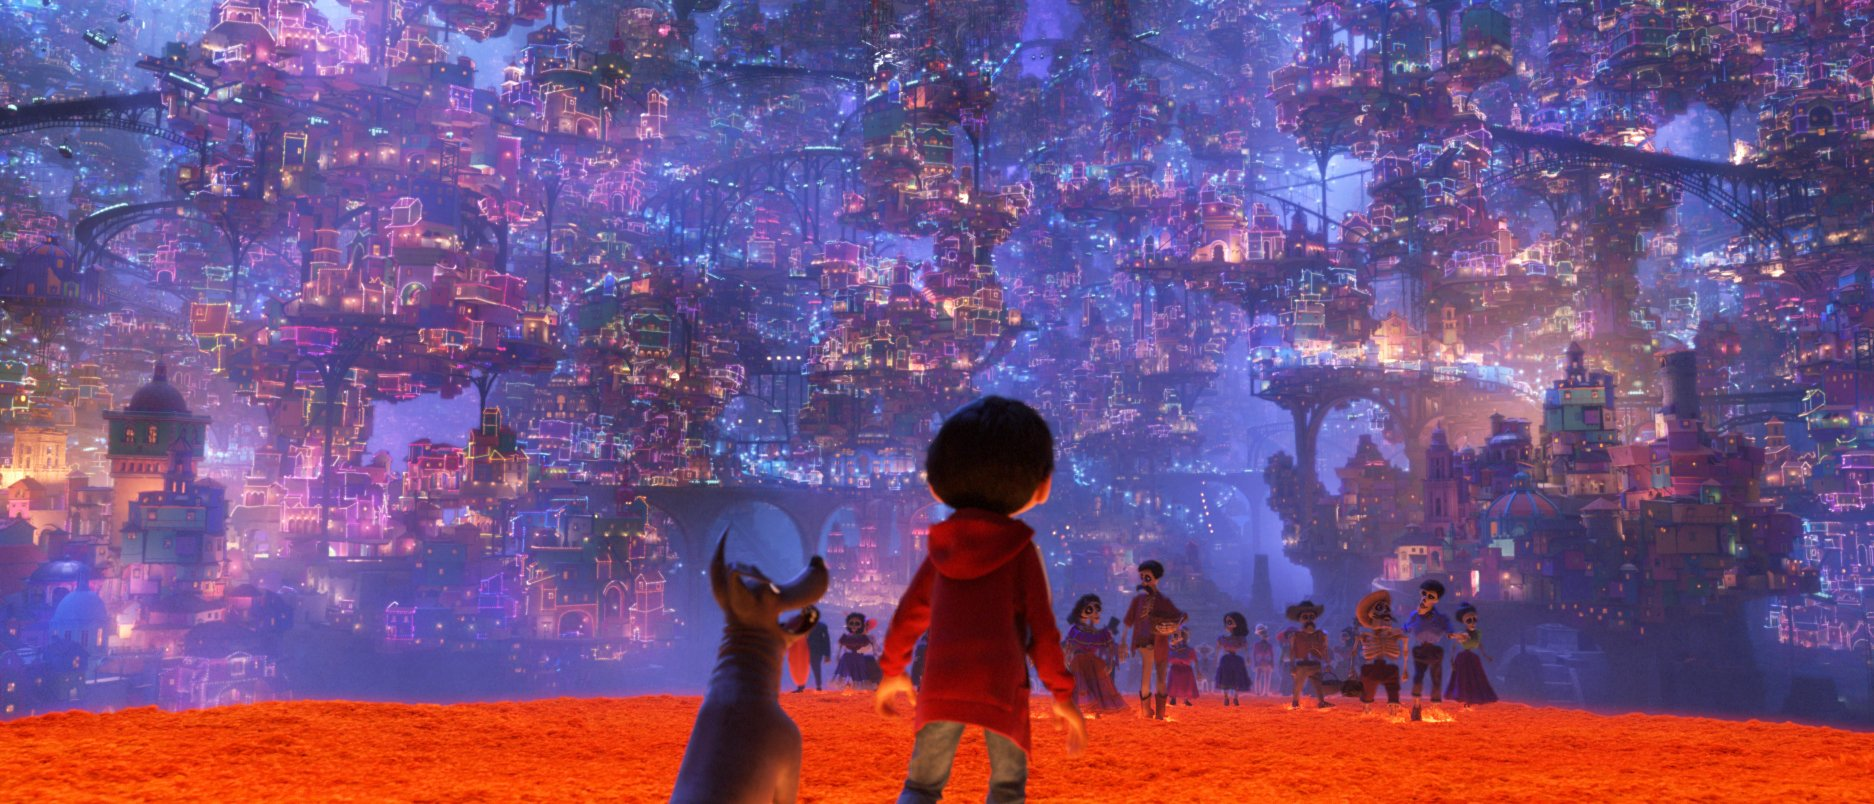
\includegraphics[width=1.0\linewidth]{img/coco1.jpg}
    \caption[A shot from the movie Coco]{A shot from Pixar's movie Coco. It shows the scene complexity that production renderers have to deal with (Image from \cite{coco}).}
    \label{fig:coco}
\end{figure}
Besides the scene geometry, textures in feature films can additionally consume up to a terabyte of memory \cite{arnold}.
While high detailed geometry and textures are required for close-up shots, they impair performance when rendering them at large distances like in a landscape scene.
This occurs because rays have to be intersected with all triangles of the high-resolution geometry, regardless of their distance to the camera.
Additionally having highly detailed geometry and textures at distance is prone to aliasing due to undersampling \cite{pbr}.
Tracing more rays per pixel combats this problem but is usually not feasible, since it increases the render time and has to be done for every frame.
Alternatively, we can use meshes with fewer triangles and textures that have less details.
Since the aliasing effect increases with distance from the camera, we generate multiple \textit{levels of detail} (\acsp{lod}) and render them at a corresponding distance.
However, selecting \acsp{lod} based on the distance from the camera is not the only possible strategy.
If scene objects have to be streamed over a network, it can be necessary to select an \ac{lod} based on the connection speed.
For example, since the memory size is proportional to the detail level, \acsp{lod} can ensure the usability of an \ac{ar} system regardless of the available bandwidth \cite{petrangeli_dynamic_adaptive_streaming}.

In this thesis we want to explore an approach for \acl{lod} rendering which combines the information of surface meshes and textures into a single representation using volumes.
We introduce fundamental concepts to the thesis in Chapter \ref{chap:fundamentals} and explain our method in Chapter \ref{chap:method}.
In Chapter \ref{chap:results_and_discussion}, we present our results and discuss them before we look at further improvements to our approach in Chapter \ref{chap:future_work}, and summarize our findings in Chapter \ref{chap:summary}.
First however, we look at the research that has been published in our domain in the following section.
\section{Related Work}
This thesis crosses several areas of research in computer graphics.
This includes the representation of dense materials by volumes, efficient volume rendering and \ac{lod} rendering.
In this section, we want to present the most relevant publications of these areas.

\subsection{Representing Dense Materials by Volumes}
Generally, the visual appearance of volumes is determined by the choice of a phase function and the density of the medium respectively its extinction \cite{pbr}.
Therefore, research mainly focuses on further improving these functions and the extinction behavior.

% The first work that suggested the use of volumes beyond the rendering of dust or smoke
Representing surfaces by volumes is a long-standing problem in computer graphics.
An early work by \citeauthor{kajiya_rendering_fur_with_textures} uses three dimensional textures of density values to render fur.
The authors store the particle density, a coordinate frame as well as parameters for diffuse and specular reflection functions in each texel.
The density is obtained from a particle system which models the flow of a hair using the particle's trajectory \cite{kajiya_rendering_fur_with_textures}.
% The diffuse lighting component is transformed from the traditional lambertian reflectance model by integrating over the half cylindrical shape of a hair that faces the light source \cite{kajiya_rendering_fur_with_textures}.
% For specular reflection the authors

In a paper by \citeauthor{meng_multi_scale_modeling_and_rendering_of_granular_materials}, volumetric representations of grains are used for efficient path tracing.
For modeling the light scattering in the volume, the authors use a tabulated phase function.
This phase function is measured from simulating the light scattering of a single grain using ray tracing.
The extinction coefficient is computed from the simulation results as well, since the authors also track the mean free-flight distance between successive interactions with grain.
Compared to the surface representation, the authors observe a speedup of 2.1-30$\times$ depending on the test scene.
The authors argue that this speedup occurs because the surface representations cannot employ next event estimation if a grain is occluded by other grains.
Therefore, paths have to be traced explicitly through the geometry if a grain does not lie on the surface \cite{meng_multi_scale_modeling_and_rendering_of_granular_materials}.

Many recent contributions use the microflake model introduced by \citeauthor{microflake}, which models a volume by two-sided, randomly oriented flakes and therefore allows anisotropic media \cite{microflake}.
\citeauthor{zhao_building_volumetric_appearance_models} use this model to render fabric \cite{zhao_building_volumetric_appearance_models}.
The authors work with real fabric and scan it using computer tomography to obtain the density values for each voxel.
To compute the orientation of the microflakes in each voxel, the authors fit cylinders to the scanned density field.
For estimating the color and reflection properties, the authors repeatedly render the volume and adjust the properties until the image matches a photograph of the fabric \cite{zhao_building_volumetric_appearance_models}.

\citeauthor{sggx} contributed another paper that uses the microflake framework.
The authors develop a new phase function which resembles the reflection properties of the GGX \ac{brdf} in volumes.
It can be used to substitute existing fiber-like scattering functions as well as surface-like scattering functions \cite{sggx}.
This property makes it interesting for our thesis, since we want to represent surface meshes by volumes.
Therefore, we explain the theoretical background extensively in Section \ref{subsec:phase_function}.

Recent research also tries to combine surface and volume reflection models into a single description.
\citeauthor{dupuy_unification_of_microfacet_and_microflake} build on the microflake framework by \citeauthor{microflake} but they use one-sided microflakes \cite{dupuy_unification_of_microfacet_and_microflake}.
These are microflakes that are transparent on one side and reflective on the other side.
The authors observe that their model allows for surface-like reflection, but it breaks the reciprocity within the medium \cite{dupuy_unification_of_microfacet_and_microflake}.

A fundamentally different approach is taken by \citeauthor{mildenhall_nerf} \cite{mildenhall_nerf}.
They use a neural network based approach to represent radiance emitted by volumes.
These neural networks take a world position $(x, y, z)$ and a view direction $(\theta, \phi)$ as input and output the RGB color and the density.
The authors call these networks \acp{nerf} and they can be rendered using classical volume rendering principles.
A limitation of their approach is that \acsp{nerf} can only represent static scenes with static lighting \cite{mildenhall_nerf}.
This sets them apart from our approach, which works for arbitrary models and changing lighting conditions.

\subsection{Efficient Volume Rendering}
Although this thesis does not provide contributions to the optimization of volume rendering itself, using optimizations is key for competing with hardware accelerated ray tracing.
A popular algorithm in volume rendering is \textit{delta tracking} \cite{woodcock}, which needs a majorant of the volume's particle density.
In its basic form this is a global majorant over the entire volume, however for strongly heterogeneous media it is more efficient to use local majorants \cite{novak_overview}.

To obtain local density majorants for delta tracking, \citeauthor{yue_space_partitioning} compare different space partitioning techniques regarding their performance implications \cite{yue_space_partitioning}.
These encompass a uniform grid partitioning, kd-trees and octrees.
The authors evaluate their schemes on $8 \times 8 \times 8$ density grids and observe the highest speed-up compared to a global density majorant for the kd-tree with up to ${50\times}$.
A drawback is the high construction time of more than $\SI{1.5}{\s}$ which is two orders of magnitudes slower than the octree and three orders of magnitudes slower than the uniform partitioning \cite{yue_space_partitioning}.

\citeauthor{brick_grid} use local density majorants for their distance sampling and transmittance estimation.
Additionally, their density majorant is available on different scales to account for high variation in the density \cite{brick_grid}.
The whole approach of \citeauthor{brick_grid} is optimized for the usage on a \ac{gpu}, which is why we use it in our research.
We go into further detail on this paper in Section \ref{subsec:solving_beer_lambert_law_in_heterogeneous_media}.

% \subsection{Mesh voxelization}
\subsection{Approaches for Level of Detail Rendering}
The theory for \ac{lod} rendering is motivated by the Nyquist-Shannon sampling theorem \cite{shannonsampling}, which states that aliasing occurs when we sample a signal with less than twice the maximum frequency of the signal.
When keeping the sampling rate constant, we can therefore avoid aliasing by reducing the maximum frequency of the signal.

As mentioned in the introduction, the usual approach to achieve this goal for textures is to use increasingly blurry textures, which is generally called mipmapping \cite{mipmapping}.
This method generates new \acsp{lod} by recursively averaging the color of four neighboring texels until one texel remains on one or both dimensions of the texture \cite{mipmapping}.
Another approach for texture \acsp{lod} is the \ac{sat} \cite{crow_summed_area_tables}.
For this method, a new texture is generated where each texel stores the sum of all texel values in the rectangle between the texel position and the lower left corner of the texture image.
It is now possible to retrieve arbitrary filtered texture values by specifying upper and lower bounds of a rectangle for which the filtered color should be calculated.
The summed intensity of the rectangle is then given by adding the value on the bottom left of the rectangle to the value on the top right, minus the values at the upper left and lower right.
Dividing the summed intensity by the area of the rectangle then gives the filtered color \cite{crow_summed_area_tables}.

For generating \acsp{lod} of surface meshes there are a number of strategies which we can classify as \textit{simplification}, \textit{subdivision}, \textit{tessellation} and \textit{voxel-based} approaches.
Even though we do not employ simplification, tessellation or subdivision in this thesis, we present them in the following, because they are widely used approaches in game engines \cite{niessner_tessellation} and feature film renderers \cite{arnold}.

% \noindent\textbf{Simplification}\linebreak
\subsubsection*{Simplification}
Mesh simplification techniques have in common that they remove geometry from an existing high detailed mesh while trying to preserve the visual appearance \cite{realtime}.
This approach is followed in a paper by \citeauthor{hoppe_simplification} \cite{hoppe_simplification}.
They formulate the problem as the minimization of an energy function 
\begin{equation*}
    E = E_{dist} + E_{rep} + E_{spring},
\end{equation*} where $E_{dist}$ measures the total squared distance of the mesh's points and $E_{rep}$ penalizes the number of vertices.
$E_{spring}$ is a regularization term, which acts as if the edges between vertices were replaced by springs.
Their algorithm randomly attempts to remove edges from the mesh and marks the change as preliminary if $E_{new} < E_{old}$.
In a second step, one of the vertices in the neighborhood to this preliminary change is moved in order to minimize $E_{dist}$ and $E_{spring}$ while omitting self-intersections of the mesh \cite{hoppe_simplification}.

\citeauthor{peng_simplification} use edge collapse in a \ac{lod} context \cite{peng_simplification}.
They first apply a pre-processing step which determines the chronological order of the edge collapse.
Based on this order, the vertices are restructured in memory, starting from vertices that exist in all \acp{lod} to vertices that only exist in detailed \acp{lod}.
This allows to only load the vertices to the GPU that are required for the current \ac{lod}.
The \ac{gpu} then applies the actual edge collapsing using one thread per triangle \cite{peng_simplification}.

% The authors of \citetitle{garland_heckbert_simplification} follow a similar approach, however they use a quadric error metric for the optimization procedure \cite{garland_heckbert_simplification}.
% \noindent\textbf{Subdivision}\linebreak
\subsubsection*{Subdivision}
Subdivision algorithms can also be seen as an instance of \ac{lod} approaches, since they start with a coarse mesh and iteratively produce smoother meshes.

\citeauthor{CATMULL1978350} introduced an algorithm that is now widely known as Catmull-Clark subdivision \cite{CATMULL1978350}.
The algorithm is not limited to triangle meshes but can be used with arbitrary polygons.
In the first step, a new \textit{face point} is computed by calculating the average position of the vertices defining the face.
Secondly, for every edge the authors compute the average position of the midpoint of this edge with the two adjacent face points generated in step one.
This gives new \textit{edge points}.
Finally new \textit{vertex points} are generated by computing:
\begin{equation*}
	\frac{Q}{n} + \frac{2R}{n} + \frac{S(n-3)}{n},
\end{equation*}
where $Q$ is the average of the $n$ new face points from step one that are adjacent to an old vertex point.
$R$ is the average of the midpoints of all old edges that are incident on the old vertex points and $S$ is the old vertex point.
% Figure \ref{fig:catmull_clark_new_points} illustrates the points that have been generated by these three steps.
Using these points, new edges are added: Each new face point is connected to the adjacent new edge points from step two.
Then the algorithm connects each new vertex point to the new edge points surrounding it \cite{CATMULL1978350}.
Figure \ref{fig:catmull_clark_subdivision} shows the subdivision of a cube after one iteration.
\begin{figure}[t]
    \centering
    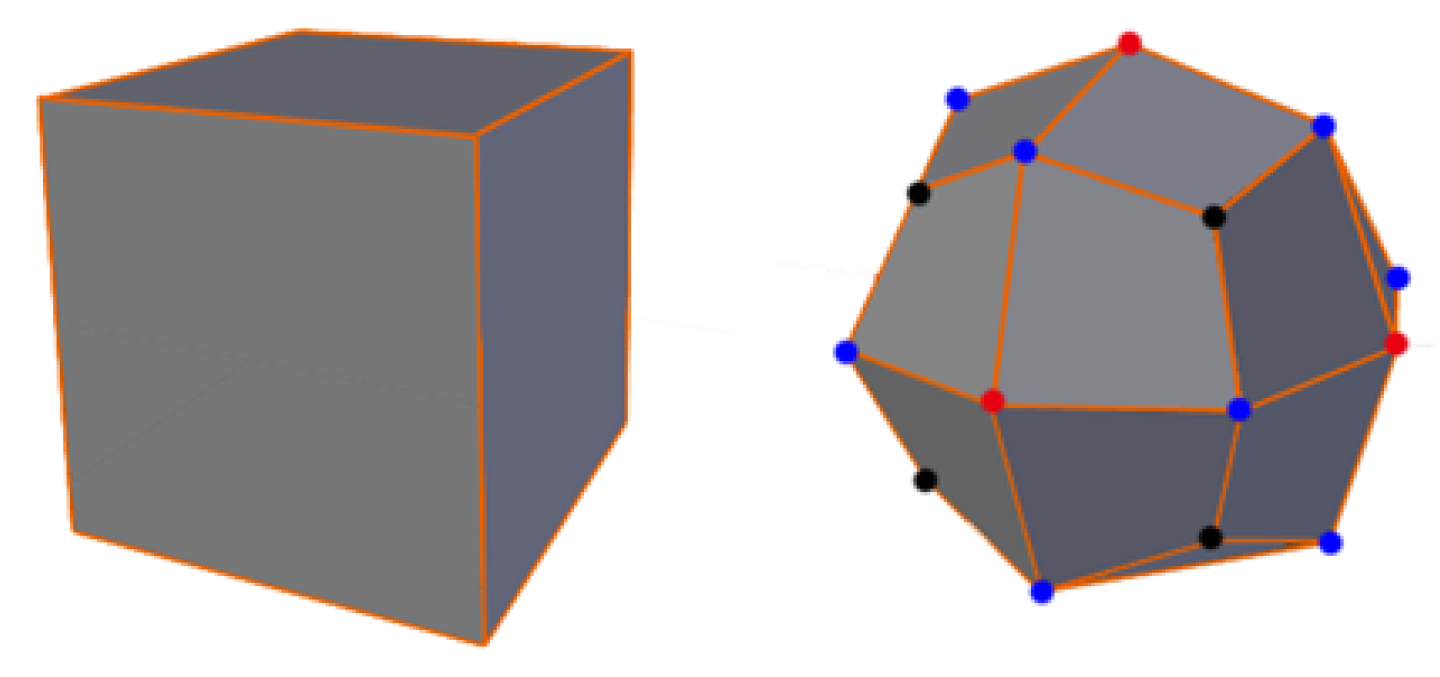
\includegraphics[width=0.5\linewidth]{img/catmull_clark_subdivision.png}
    % \caption[Points generated by the Catmull-Clark subdivision]{Points generated after the first three steps of the Catmull-Clark subdivision. Blue: Face points, generated in the first step. Pink: Edge points, generated in second step. Green: Vertex points, generated in third step. (Image from \cite{catmull_clark_step_3}).}
    \caption[First iteration of the Catmull-Clark subdivision]{First iteration of the Catmull-Clark subdivision on a cube mesh. The colors show in which step the point was generated. Red: Face points, generated in the first step. Blue: Edge points, generated in second step. Black: Vertex points, generated in the third step (Image from \cite{cheng_catmull_clark_visualization}).}
    \label{fig:catmull_clark_subdivision}
\end{figure}

\citeauthor{loop_subdivision} later proposed another algorithm for triangle meshes \cite{loop_subdivision}.
In a first step, a new vertex is added at the midpoints of each edge.
Then the positions of existing and new vertices are updated using the weights in Figure \ref{fig:loop_subdivision}.
For existing points, the new position is a weighted sum of all the surrounding vertices as well as the old position of the vertex.
New points take the immediate neighboring points into account as well as the other two points that form the adjacent triangles.
The weight $\beta$ is given by \cite{loop_subdivision}:
\begin{equation*}
    \beta = \frac{1}{n}(\frac{5}{8} - (\frac{3}{8} + \frac{1}{4}cos(\frac{2\pi}{n}))^2).
\end{equation*}
\begin{figure}[t]
    \centering
    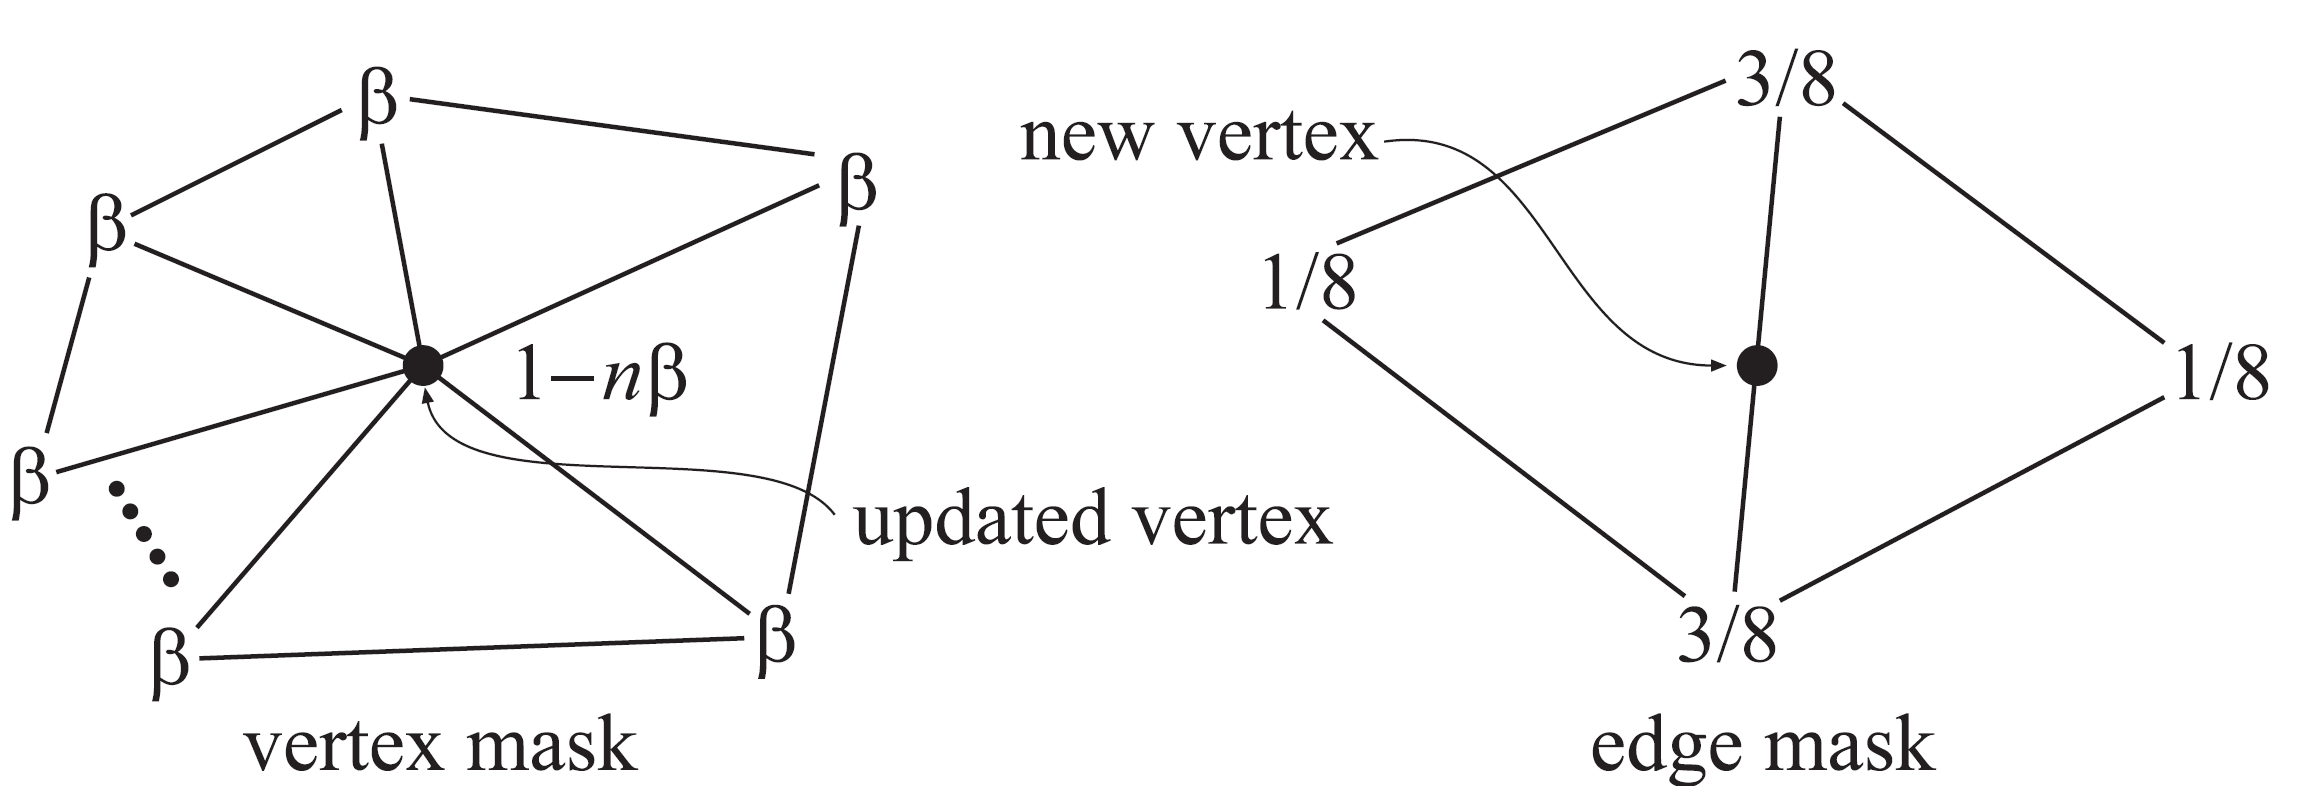
\includegraphics[width=0.5\linewidth]{img/loop_subdivision.png}
    \caption[Weights in Loop subdivision]{The weights for updating existing and new vertices in Loop subdivision. For existing points, the weight depends on the valence $n$ and a weight $\beta$, while new vertices are updated with constant values. (Image from \cite{realtime}).}
    \label{fig:loop_subdivision}
\end{figure}

\citeauthor{niessner_subdivision} explore how Catmull-Clark subdivision can be implemented on a \ac{gpu} \cite{niessner_subdivision}.
The authors use a table-driven approach, where they first analyze the mesh on the \ac{cpu} and store the indices of the vertices that contribute to a subdivision in a table.
Using this data, they determine the new face, edge and vertex points with compute kernels on the \ac{gpu} by launching a thread for each new point.
\citeauthor{niessner_subdivision} find that supporting this process with hardware tessellation for all regular faces improves the performance of their algorithm \cite{niessner_subdivision}.


\subsubsection*{Tessellation}
Tessellation is similar to subdivision, as it also increases the number of triangles of a coarse mesh.
It typically refers to hardware tessellation which is a part of the rendering pipeline of modern \acp{gpu}.


An early work by \citeauthor{moreton_tessellation} compares the De Casteljau and the forward differencing algorithm for evaluating tensor product surfaces \cite{moreton_tessellation}.
These parametric surfaces are the basis for hardware tessellation.
The authors find that the De Casteljau algorithm produces more stable and precise results and supports evaluation at arbitrary parameter values.
Forward differencing only uses additions and has a complexity of $O(n)$ compared to a complexity of $O(n^2)$ for the De Casteljau algorithm.
This comes at the cost of being less precise and requiring a fixed parametric interval.
Since the authors do not require the precision of De Casteljau they use forward differencing and propose a hardware implementation for the algorithm.
The authors also present a way to produce continuous \acp{lod} by using fractional tessellation.
For that the tessellation is no longer uniform \cite{moreton_tessellation}.

An extensive overview of modern hardware tessellation is given in a paper by \citeauthor{niessner_tessellation} \cite{niessner_tessellation}.
The authors show how tessellation integrates into current rendering pipelines as it is performed after the vertex shader and before the geometry shader.
The first step is the hull shader which controls the tessellation rate of the parametric surface patch.
For quads, four outer and two inner factors can be specified, while for triangles, three outer and one inner factor is available.
Following the hull shader, the fixed function tessellator generates sample points and topology for a patch domain based on the tessellation factors.
Finally, the domain shader is executed for each sample location.
It computes vertex attributes based on the tessellation factor, control points and domain sample locations.
The authors also present various evaluation procedures for tensor product surfaces \cite{niessner_tessellation}.

\subsubsection*{Voxel-Based}
Compared to the \ac{lod} approaches described before, voxel-based approaches can not only encode the geometry of a model but also their texture.

\citeauthor{afra_voxel_lods} applies surface voxelization to large meshes with hundreds of millions of triangles \cite{afra_voxel_lods}.
The authors start by subdividing the geometry to build a kd-tree until each node in the tree contains no more than one triangle.
Starting from the root, voxelization is then performed on every third level for nodes with more than one triangle.
Their voxelization procedure is based on rasterization, where the triangles within a voxel are projected to all six sides of the voxel.
The authors then average normals and colors and store this average if the maximum absolute difference between the samples and the average is below a threshold.
If that is not the case, all six samples are stored.
The resulting kd-tree represents inner nodes using voxels and the leaves are represented by single triangles.
\citeauthor{afra_voxel_lods} then renders the scene using ray tracing against the kd-tree.
The tree is traversed and for every voxel node, the screen space area of that node respectively the voxel is computed to determine whether to continue traversal \cite{afra_voxel_lods}.

Compared to \citeauthor{afra_voxel_lods}, \citeauthor{hybrid_mesh_volume_lods} propose a method for generating physically plausible density values for each voxel \cite{hybrid_mesh_volume_lods}.
The authors use a hybrid approach between mesh and volume \acp{lod}.
Their idea is to represent macroscopic surfaces (larger than the target resolution) as mesh \acsp{lod} while microscopic geometry (smaller than the target resolution) is represented by volumes.
The first step in their pipeline is the separation of the macroscopic from the microscopic geometry.
For example, the trunk of a tree would be separated from its branches and leaves.
The second step is to apply mesh simplification on the macroscopic surface while preserving the reflectance properties.
The authors achieve mesh simplification by using edge collapse, therefore they remove triangle edges which are smaller than the target resolution.
To preserve reflectance, the authors update the diffuse and specular albedos of the remaining vertices by a weighted sum of the old vertices.
The last step in their pipeline is the voxelization of the sub-resolution geometry.
The authors choose a ray casting approach to estimate the density for each voxel.
This provides artifact-free voxelization and is therefore interesting for our research \cite{hybrid_mesh_volume_lods}.
We go into more detail about their filtering procedure in Section \ref{sec:transforming_meshes_into_volumes}.





\section{Contributions}
Our work provides the following contributions:
\begin{itemize}
    \item Implementation of a \ac{gpu} accelerated application for transforming triangle meshes into preferably equivalent volumetric representations in different resolutions and storing these representations in a usual format.
    \item Extending these volumetric representations by attributes like color, normals and other material properties to approximate surfaces more closely.
    \item Implementation of a \ac{gpu} based renderer capable of rendering surface meshes and volumes.
    \item An empirically motivated heuristic to determine which \ac{lod} should be rendered.
    \item A scene generator that generates forest scenes, incorporating the heuristic for \ac{lod} selection.
    \item Evaluation of the tradeoff between image quality, rendering performance and memory consumption when triangle meshes are approximated by volumetric \acsp{lod}.
\end{itemize}
 

\chapter{Fundamentals}
\label{chap:fundamentals}
This chapter introduces the fundamental concepts necessary for the thesis.
We use these notations throughout the thesis:
\begin{center}
    \begin{tabular}{ l  l }
        % \hline
        Notation & Definition \\
        \hline
        $\omega_i$ & Direction from a point of interaction towards the light source \\
        % \hline
        $\omega_o$ & Direction from a point of interaction towards the camera \\
        $\omega_h$ & Half vector: $\omega_h=\frac{\omega_i + \omega_o}{||\omega_i + \omega_o||}$ \\
        % \hline
        Bold letters ($\boldsymbol{x}$, $\boldsymbol{y}$, ...) & Points in space \\
        % \hline
        $n_{\boldsymbol{x}}$ & The normal at point $\boldsymbol{x}$ \\
        $\mathcal{H}^2$ & Hemispherical integration domain \\
        $\mathcal{S}^2$ & Spherical integration domain \\
        % \hline
    \end{tabular}
\end{center}

\section{Surface Path Tracing}
We aim to implement a physically based renderer in order to validate the results of our experiments.
The key property of physically based approaches is the conservation of energy which is given by the rendering equation \cite{rendering_equation}:
\begin{equation}
    \label{eq:render_equation}
    L(\boldsymbol{x}, \omega_o) = L_e(\boldsymbol{x}, \omega_o) + \int_{\mathcal{H}^2} f(\boldsymbol{x}, \omega_o, \omega_i) L(\boldsymbol{y}, -\omega_i) |n_{\boldsymbol{x}} \cdot w_i| d\omega_i.
\end{equation}
It states that the radiance at a point $\boldsymbol{x}$ in direction $\omega_o$ is given by the emitted radiance at this point plus the integral over the hemisphere $\mathcal{H}^2$ of the \ac{brdf} $f$ times the radiance $L$ coming from a point $\boldsymbol{y}$ in direction $\omega_i$ times the absolute value of the dot product between the normal $n_{\boldsymbol{x}}$ and the incident direction $\omega_i$.
Since this equation is generally not analytically solvable, we use Monte Carlo integration to solve it numerically.
For that we have to replace the integral by a sum and divide each summand by the number of summands and by the probability of creating a sample $i$ \cite{pbr}:
\begin{equation*}
    L(\boldsymbol{x}, \omega_o) = L_e(\boldsymbol{x}, \omega_o) + \frac{1}{N}\sum_{i=1}^{N} \frac{f(\boldsymbol{x}, \omega_o, \omega_i) L(\boldsymbol{y}, -\omega_i) |n_{\boldsymbol{x}} \cdot w_i|}{p(\omega_i)}.
\end{equation*}
The recursive nature of this equation can be observed immediately, as we could substitute the radiance $L$ in the sum by the whole equation.
However, implementing the algorithm this way is infeasible since that would lead to exponential growth of compute time and memory consumption with recursion depth.
As a solution to this problem \citeauthor{rendering_equation} proposed the \textit{path tracing} algorithm \cite{rendering_equation}.
Instead of sampling $N$ new directions at each point of intersecting the geometry, we sample a single direction at each intersection point starting at the camera until we hit a light source.
Conceptually the recursive approach spans up a ray tree.
In this tree the root represents the camera, a new level is added at each point of reflection and the leaves are light hits.
Path tracing then only samples one path from the root to a light source in this tree \cite{rendering_equation}.
Sampling only one path is a bad estimate of the integral, but when we repeat this process a large number of times we still get the same result as with using the recursive approach \cite{pbr}.
Additionally, there are methods to reduce the variance of the paths like importance sampling or next event estimation.
In short, importance sampling reduces variance by sampling from a distribution that has a similar shape like the integrand of Equation \ref{eq:render_equation} \cite{rendering_equation}.
Thus, for importance sampling $L$ we could, for example, sample an environment map and mostly generate rays towards the sun, while importance sampling $f$ requires to preferably generate rays in directions where $f$ is large.
Next event estimation, on the other hand, computes the direct illumination from a light source at each path vertex, by importance sampling this light source \cite{pbr}.
\citeauthor{pbr} provide detailed explanations of these techniques \cite{pbr}.

\section{Volumetric Path Tracing}
The rendering equation introduced in Equation \ref{eq:render_equation} is only valid for light transport in a vacuum.
Since we want to represent our \acsp{lod} by volumes, we now extend this formulation to be able to render heterogeneous volumes.
Formally, volumes have a density ${\rho > \SI{0}{\frac{1}{\m^3}}}$ \cite{pbr}.
Thus, $\rho$ gives us the number of particles in a unit volume.
Using a particle density allows us to model the particles statistically, instead of explicitly modeling every single particle \cite{novak_overview}.
We store the density values in discrete regions of space, which are called \textit{voxels} \cite{pbr}.
These voxels can then be arranged in three dimensional grids \cite{pbr}.
Although it is conceptually helpful to think of volumes as these \textit{dense grids} it leads to redundant memory, since vacuum regions must still be stored.
For example, if we approximate the volume of a sphere by a dense grid, $1 - \frac{V_{sphere}}{V_{cube}} = 1 - \frac{\frac{4}{3}r^3\pi}{(2r)^3}\approx \SI{48}{\%}$ of the voxels will store a density of zero.
Therefore, we would like to store relevant values only, which is called a \textit{sparse grid}.
\citeauthor{museth_vdb} uses this approach in the OpenVDB library and stores the grid in a B+tree \cite{museth_vdb}.
For fast traversal, leaves and internal nodes still use dense arrays but the root node is represented by a hash table to allow for a dynamic number of voxels.
Compared to the dense grid, the background value is just stored once in the root node \cite{museth_vdb}.
A \ac{gpu} compatible port of OpenVDB is NanoVDB.
It removes third-party dependencies of OpenVDB and is designed as a header-only library.
In memory, the hierarchical tree is represented continuously without any pointers, which allows for fast copying between \ac{cpu} and \ac{gpu} and cache-friendly traversal on the \ac{gpu} \cite{museth_nanovdb}.

\subsection{Theory of Light Propagation in Participating Media}
\label{subsec:theory_of_light_propagation_in_participating_media}
For volumes, the radiance along a ray is determined by the in- and out-scattering as well as the emission and absorption properties of the medium as visualized in Figure \ref{fig:novak_volume_effects}.
\begin{figure}[t]
    \centering
    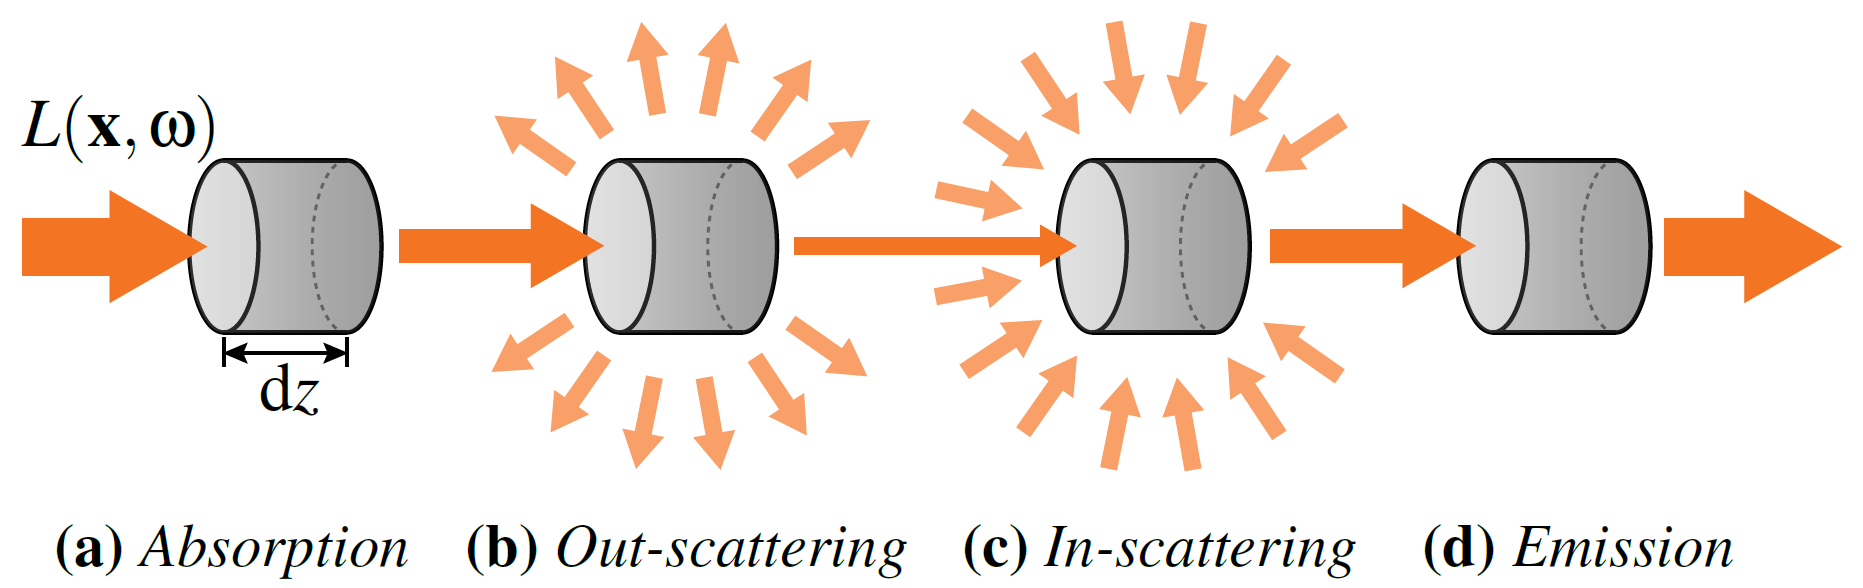
\includegraphics[width=0.7\linewidth]{img/novak_volume_effects.png}
    \caption[Physical effects in a volume]{The physical effects that are modeled by the \textit{radiative transfer equation}. \textit{Absorption} and \textit{our-scattering} reduce the radiance along a ray, \textit{in-scattering} and \textit{emission} increase the radiance (Image from \cite{novak_overview}).}
    \label{fig:novak_volume_effects}
\end{figure}
These effects are quantified by the \textit{scattering coefficient} $\mu_s$ and the \textit{absorption coefficient} $\mu_a$.
The sum of $\mu_s$ and $\mu_a$ is called the \textit{extinction coefficient} $\mu_t=\mu_a + \mu_s$, and accounts for either of the effects.
These coefficients are related with the density $\rho$ by the \textit{cross-sectional areas} $\sigma$ of the particles, thus for the scattering coefficient we have: $\mu_s = \rho \sigma_s$.
We can further define the fraction of photons that scatter as the \textit{albedo} $\alpha=\frac{\mu_s}{\mu_t}$ \cite{novak_overview}.
With the integral form of the \textit{radiative transfer equation}, we have a way to formalize the scattering, emission and absorption of the medium \cite{novak_overview}:
\begin{equation}
    \begin{split}
        \label{eq:radiative_transfer}
        L(\boldsymbol{x}, \omega_o) = \int_0^\infty T(t)[\mu_a(\boldsymbol{y})L_e(\boldsymbol{y}, \omega_o) + \mu_s(\boldsymbol{y})L_s(\boldsymbol{y}, \omega_o)]dy & \;\text{with}\; \boldsymbol{y}=\boldsymbol{x} + y\omega_o \\
                                                                                                                                                                    & \;\text{and}\; t=||\boldsymbol{x}-\boldsymbol{y}||.
    \end{split}
\end{equation}
$T$ denotes the transmittance over the distance $t$ (Beer-Lambert law \cite{lambert}) and $L_s$ is the in-scattered radiance which accounts for the radiance scattered into the medium from all directions \cite{novak_overview}:
% \begin{multicols}{2}
% \end{multicols}
% \noindent\begin{minipage}{.5\linewidth}
% \end{minipage}
% \begin{minipage}{.5\linewidth}
% \end{minipage}
\begin{equation}
    \label{eq:beer_lambert_law}
    T(t) = e^{-\int_0^t \mu_t(\boldsymbol{x} + s\omega_o)ds},
\end{equation}
\begin{equation}
    \label{eq:in_scattered_radiance}
    L_s(\boldsymbol{x}, \omega_o) = \int_{\mathcal{S}^2} f_p(\omega_o, \omega_i)L_i(\boldsymbol{x}, \omega_i)d\omega_i.
\end{equation}
$f_p$ is called the \textit{phase function} and will be explained in Section \ref{subsec:phase_function}.

Now that we defined how light propagates in a medium, we can combine the formulation in Equation \ref{eq:radiative_transfer} with the surface formulation from Equation \ref{eq:render_equation}.
We therefore clip the upper integration bound of Equation \ref{eq:radiative_transfer} to a distance $z$ and add the attenuated surface term \cite{novak_overview}:
\begin{equation*}
    L(\boldsymbol{x}, \omega_o) = \int_0^z T(\boldsymbol{x}, \boldsymbol{y})[\mu_a(\boldsymbol{y})L_e(\boldsymbol{y}, \omega_o) + \mu_s(\boldsymbol{y})L_s(\boldsymbol{y}, \omega_o)]dy + T(\boldsymbol{x}, \boldsymbol{z})L(\boldsymbol{z}, \omega_o).
\end{equation*}
The idea of this \textit{volume rendering equation} is that a ray passing through a medium will hit a surface at distance $z$.
The integral on the right side of this equation accounts for the in-scattering and emission of the medium while the added term represents attenuated radiance arriving from the surface at distance $z$ \cite{novak_overview}.

\subsection{Solving the Beer-Lambert Law in Heterogeneous Media}
\label{subsec:solving_beer_lambert_law_in_heterogeneous_media}
As described in Section \ref{subsec:theory_of_light_propagation_in_participating_media}, effects like scattering and absorption occur when light interacts with the particles of a medium.
We therefore need a way to sample interactions on which the light then is scattered or absorbed.
At distance $t$, the Beer-Lambert law from Equation \ref{eq:beer_lambert_law} gives us the proportion of light that did not hit a particle $P(X > t) = T(t)$ \cite{novak_overview}.
Therefore, we can compute the fraction of light that hit a particle by \cite{novak_overview}:
\begin{equation*}
    F(t) = 1 - T(t).
\end{equation*}
For a homogeneous medium the probability of hitting a particle is:
\begin{equation*}
    F(t) = 1 - e^{\mu_t t},
\end{equation*}
since $\mu_t$ is constant in the whole medium.
After rearranging, this gives us a method to sample free path distances in homogeneous media:
\begin{equation}
    \label{eq:distance_sampling}
    t(\xi) = -\frac{ln(1-\xi)}{\mu_t},
\end{equation}
where $\xi$ is a uniform random number in the interval $[0, 1)$ \cite{novak_overview}.

However, distance sampling in heterogeneous media is more complex, since $\mu_t$ is spatially varying.
We could interpret each voxel as a homogeneous medium and sample a target transmittance in the interval $(0, 1]$.
We then have to accumulate the transmittance over all voxels that a ray passes until it falls below the target transmittance \cite{novak_overview}.
This method is called \textit{regular tracking} \cite{sutton_regular_tracking}.
The drawback is, that we have to compute intersections with every voxel along the ray, which can be expensive for detailed volumes \cite{novak_overview}.
Another approach is called \textit{ray marching} \cite{perlin_hypertexture}, where we traverse the medium at a constant step size.
Again, we accumulate the transmittance until it falls below a sampled target transmittance.
This method can reduce the cost compared to regular tracking but introduces bias, since it assumes a constant density between each step \cite{novak_overview}.
An unbiased approach that does not require intersection tests with voxels is \textit{Woodcock tracking} \cite{woodcock}, usually called \textit{delta tracking}.
Figure \ref{fig:novak_distance_sampling} visualizes all tree approaches.
\begin{figure}[t]
    \centering
    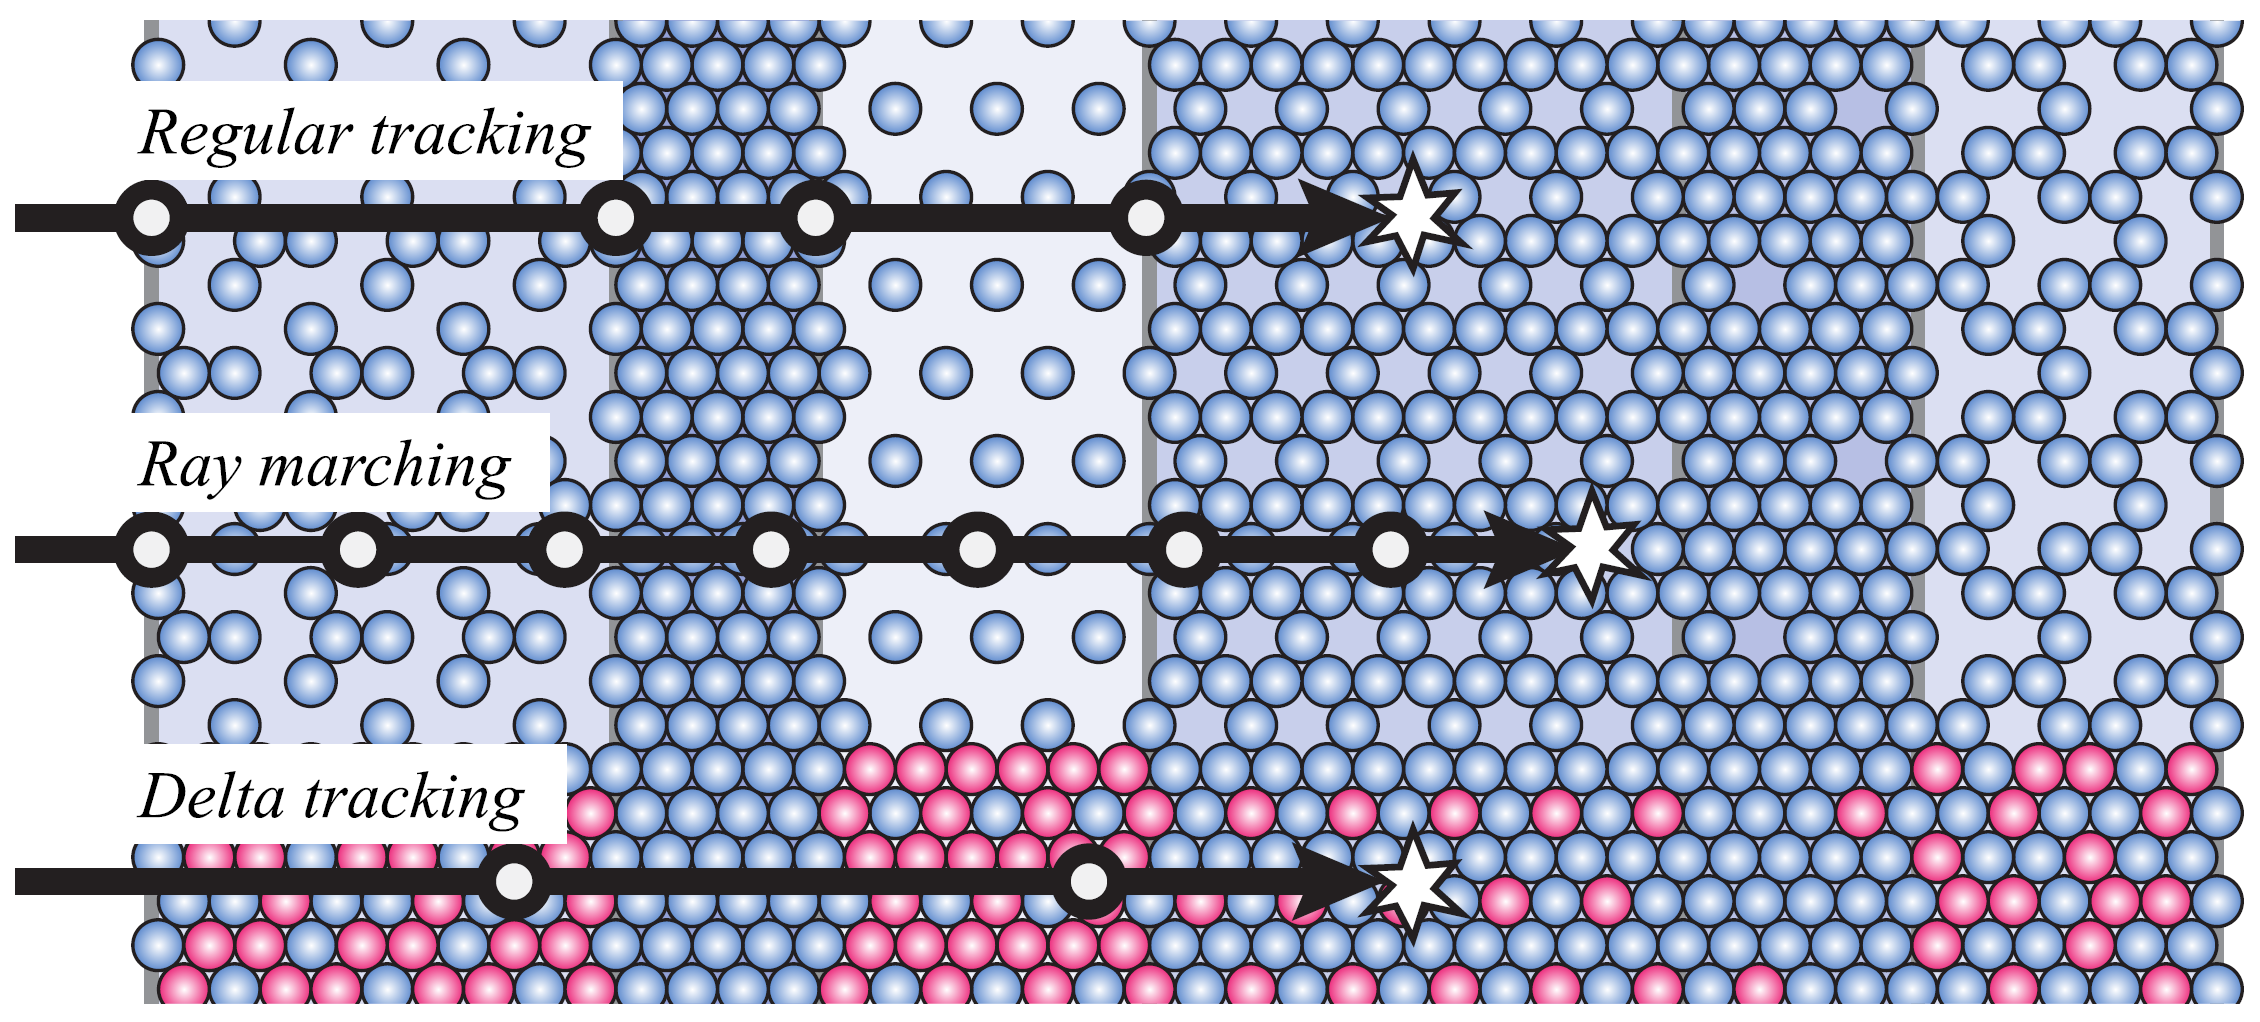
\includegraphics[width=0.7\linewidth]{img/novak_distance_sampling.png}
    \caption[Approaches for distance sampling in heterogeneous media]{Three approaches for distance sampling in heterogeneous media: Regular tracking gives exact results but requires intersections with voxel boundaries. Ray marching can reduce compute time but introduces a bias. For delta tracking we add fictious matter (red circles) to obtain a homogeneous medium and get an unbiased result (Image from \cite{novak_overview}).}
    \label{fig:novak_distance_sampling}
\end{figure}
We first have to homogenize the medium by adding fictious matter until the extinction reaches the majorant of the real matter $\bar{\mu_t}$.
This fictious matter does not influence the scattering or absorption behavior \cite{novak_overview}.
We can then iteratively sample new distances using Equation \ref{eq:distance_sampling} with $\mu_t=\bar{\mu_t}$ and compare the local extinction coefficient $\mu_t(\boldsymbol{x})$ with the majorant $\bar{\mu_t}$ using a uniform random number $\xi\in[0,1)$.
If $\xi<\frac{\mu_t(\boldsymbol{x})}{\bar{\mu_t}}$ we found a hit with a real particle and can exit the iteration, if $\xi>=\frac{\mu_t(\boldsymbol{x})}{\bar{\mu_t}}$ we found a collision with a null particle meaning that we have to continue with sampling a new distance $t$ \cite{spectral_and_decomposition_tracking}.
Note, that for a constant cross-sectional area $\sigma_t$ we can use the ratio between the local density $\rho(\boldsymbol{x})$ and the density majorant $\bar{\rho}$ instead.
To estimate the transmittance in a heterogeneous medium we employ a similar algorithm called \textit{ratio tracking}.
As opposed to delta tracking, ratio tracking does not compare whether the interaction is a null-collision.
Instead, it updates the transmission with $T_{new} = T_{old}(1 - \frac{\mu_t(\boldsymbol{x})}{\bar{\mu_t}})$ \cite{novak_ratio_tracking}.

Since both algorithms use a global majorant of the extinction, they perform poorly in media where the extinction varies strongly across the medium.
Therefore, we use local majorants as suggested by \citeauthor{brick_grid} \cite{brick_grid}.
This idea is visualized in Figure \ref{fig:brick_grid_majorants}.
\begin{figure}[t]
    \centering
    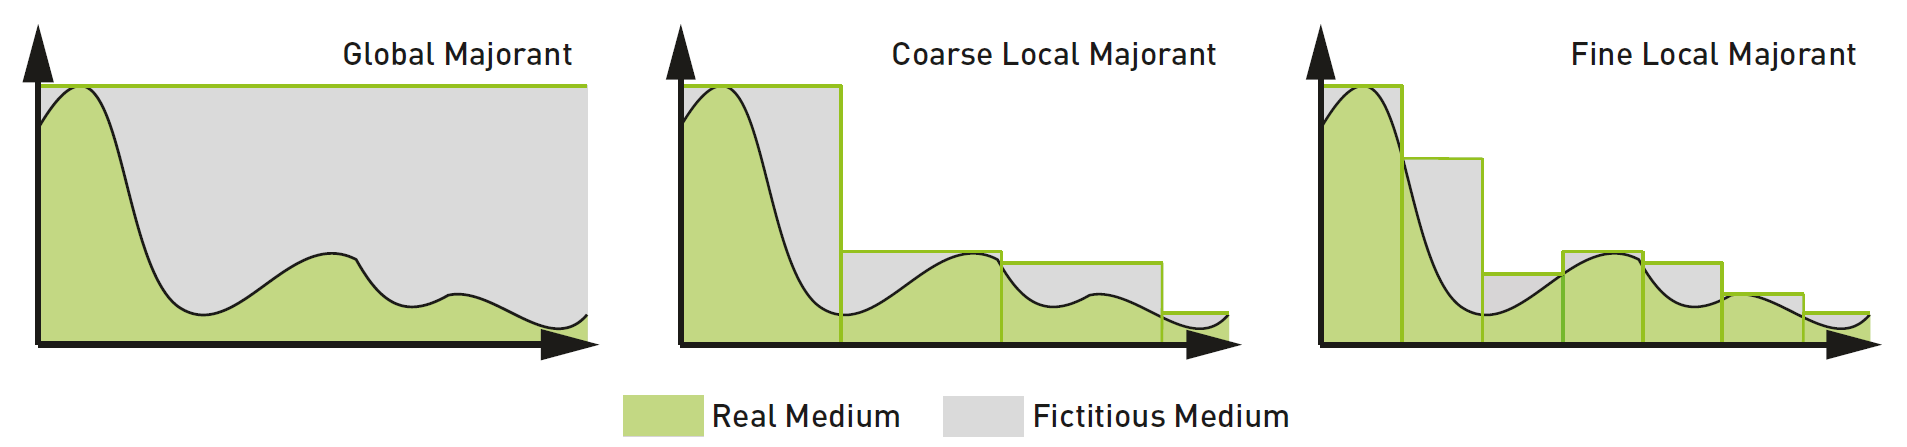
\includegraphics[width=0.9\linewidth]{img/brick_grid_majorants.png}
    \caption[Visualization of local density majorants]{Visualization of the concept of local majorants. These allow to sample distances and estimate transmittance more efficiently (Image from \cite{brick_grid}).}
    \label{fig:brick_grid_majorants}
\end{figure}
To store the volume data, we use three textures.
First, we use an \textit{atlas texture} to store \textit{bricks} which are groups of $8 \times 8 \times 8$ voxels \cite{brick_grid}.
The second texture is the \textit{indirection texture} which stores offsets into the atlas.
This texture therefore links a position in space to a brick of data in the atlas \cite{brick_grid}.
Finally we store the minorant and majorant of each brick in the \textit{range texture} \cite{brick_grid}.
These are used to scale the density values in the atlas texture to the interval $[0, 1]$ \cite{brick_grid}.
The range texture additionally has three mipmap levels which allows to have local majorants at different scales \cite{brick_grid}.
Since the resulting atlas texture no longer has spatial coherence, hardware interpolation by the texture unit is not possible \cite{brick_grid}.
Therefore, we employ a form of stochastic lookup where we jitter the lookup point by $\pm0.5$ voxels before performing point sampling \cite{brick_grid}.
When having a large number of lookups, as it is the case in Monte Carlo integration, this procedure is equivalent to trilinear interpolation without introducing a significant overhead \cite{brick_grid}.
In Figure \ref{fig:brick_grid_datastructure} we show the introduced textures visually.
\begin{figure}[t]
    \centering
    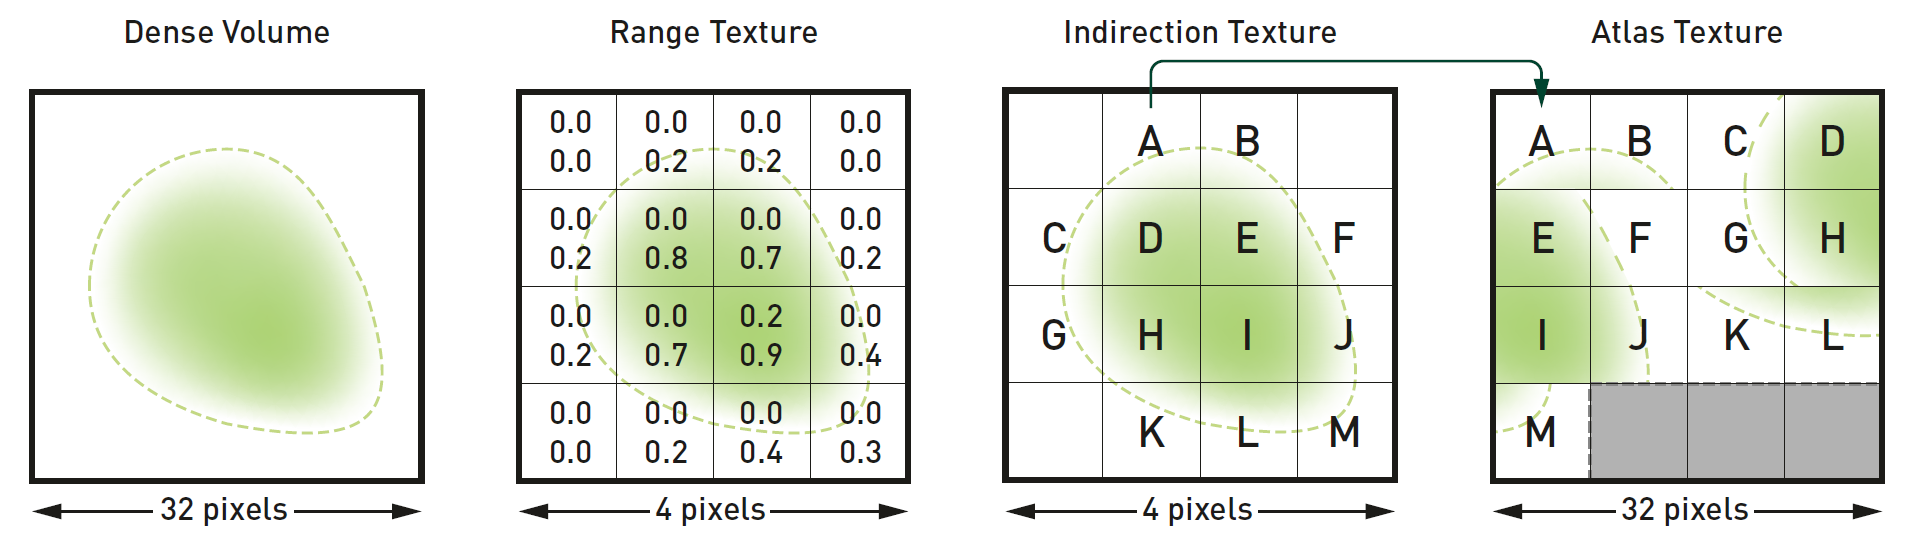
\includegraphics[width=0.9\linewidth]{img/brick_grid_datastructure.png}
    \caption[Data structure of brick grid]{Visualization of the internal data structure of brick grid. It uses a range texture, containing minorants and majorants and an indirection texture which links world positions to the density values in the atlas texture (Image from \cite{brick_grid}).}
    \label{fig:brick_grid_datastructure}
\end{figure}

For distance sampling and transmittance estimation we first sample a target optical thickness $\tau_{target}=-ln(1-\xi)$ \cite{brick_grid}.
We then accumulate the optical thicknesses of all bricks along a ray until the accumulated thickness exceeds the target thickness \cite{brick_grid}.
In this case we step back along the ray until it matches $\tau_{target}$ \cite{brick_grid}.
Now we perform the stochastic null-collision test by comparing the density at this point with the local majorant \cite{brick_grid}.
In the case of distance sampling, we return the distance to the first real collision \cite{brick_grid}.
For transmittance estimation, we adjust the current estimate by the ratio of real to fictious matter \cite{brick_grid}.
When having a null-collision, the algorithm is restarted by sampling a new target optical thickness \cite{brick_grid}.
This is repeated until a distance is successfully sampled, the transmittance estimation is stopped by Russian roulette or when the ray left the volume \cite{brick_grid}.

\subsection{Phase Functions}
\label{subsec:phase_function}
In Equation \ref{eq:in_scattered_radiance} the term of a \textit{phase function} was already introduced.
Now we want to explain this concept in more detail.
% Similar like a \acs{brdf} gives the amount of light scattered into a certain direction on a surface, a phase function gives this amount in a volume when an interaction with a particle occurs \cite{novak_overview}.
Analogous to how the \ac{brdf} describes how light is scattered when interacting with a surface, the phase function models how light scatters when an interaction with a particle occurs \cite{novak_overview}.
Opposed to \acsp{brdf}, phase functions are normalized over the unit sphere $\mathcal{S}^2$, therefore they can be seen as \acsp{pdf} as well \cite{pbr}.
For the isotropic case, meaning that light is scattered in all directions with equal probability, we can ensure the normalization by dividing with the integration domain, which is $4\pi$ for the unit sphere \cite{pbr}.
This gives us the isotropic phase function \cite{novak_overview}:
\begin{equation*}
    f_p(\omega_o, \omega_i)=\frac{1}{4\pi}.
\end{equation*}
As it can be seen the function has a constant value for all directions $\omega_o$, $\omega_i$ on the unit sphere \cite{novak_overview}.

Since we want our \acp{lod} to look similar to the corresponding mesh representation, an isotropic phase function is not sufficient.
Instead, we choose the \acs{sggx} phase function \cite{sggx} because it provides scattering properties that match diffuse and specular \acsp{brdf}.
It is particularly similar to microfacet models like the GGX \acs{brdf} \cite{ggx} which also led to the name \acf{sggx} \cite{sggx}.
The idea behind the GGX \ac{brdf} and other microfacet models is that a surface can be modeled by a distribution of normals which describe the roughness of the surface at a certain point \cite{ggx}.
Expanding on this idea, \citeauthor{microflake} \cite{microflake} introduced the microflake framework, which models the medium as two-sided specularly reflecting flakes, which are distributed according to a certain \ac{ndf}.
\citeauthor{sggx} \cite{sggx} define the \ac{ndf} for the SGGX phase function as:
\begin{equation*}
    D(\omega_m)=\frac{1}{\pi \sqrt{|S|}(\omega_m^T S^{-1} \omega_m)^2},
\end{equation*}
where $\omega_m$ is the direction of the microflake normal and $S$ is a 3 $\times$ 3 symmetric positive definite matrix which encodes the scattering properties.
This matrix is computed from the GGX roughness value $\alpha$ and the normal $n$ of the surface it should represent as
\begin{equation*}
    S=\begin{pmatrix}x^2 & xy & xz \\ xy & y^2 & yz \\ xz & yz & z^2\end{pmatrix} + \alpha^2\begin{pmatrix}y^2 + z^2 & -xy & -xz \\ -xy & x^2+z^2 & -yz \\ -xz & -yz & x^2+y^2\end{pmatrix},
\end{equation*}
where $x$, $y$, $z$ are the components of the normal $n$ \cite{sggx}.
The \ac{ndf} $D(\omega_m)$ can be seen as the extension of the GGX \acs{ndf} to the negative hemisphere as Figure \ref{fig:sggx_ndf} shows.
\begin{figure}[t]
    \centering
    \begin{subfigure}[b]{0.45\linewidth}
        \centering
        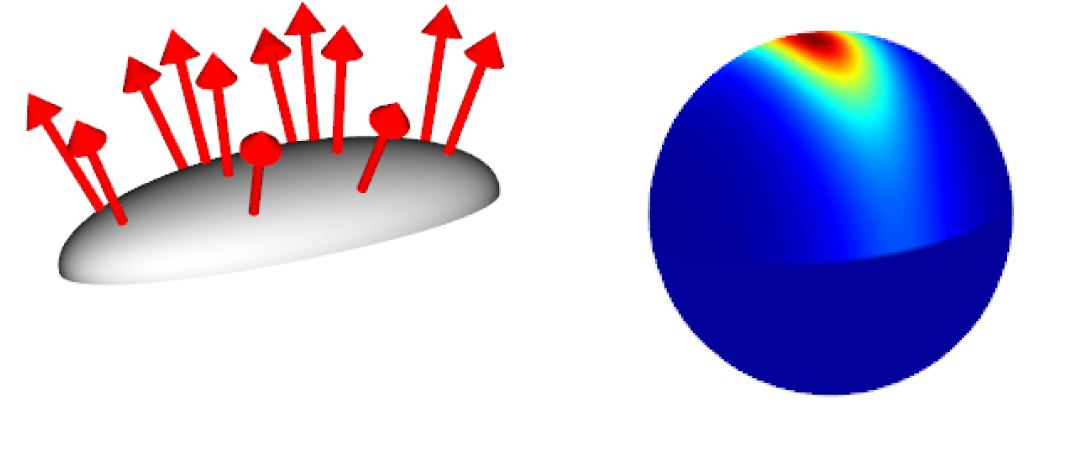
\includegraphics[width=\linewidth]{img/sggx_ndf_a.jpg}
        \caption{GGX $D(\omega_m), \omega_m \in \mathcal{H}^2$}
        \label{fig:sggx_ndf_a}
    \end{subfigure}
    \begin{subfigure}[b]{0.45\linewidth}
        \centering
        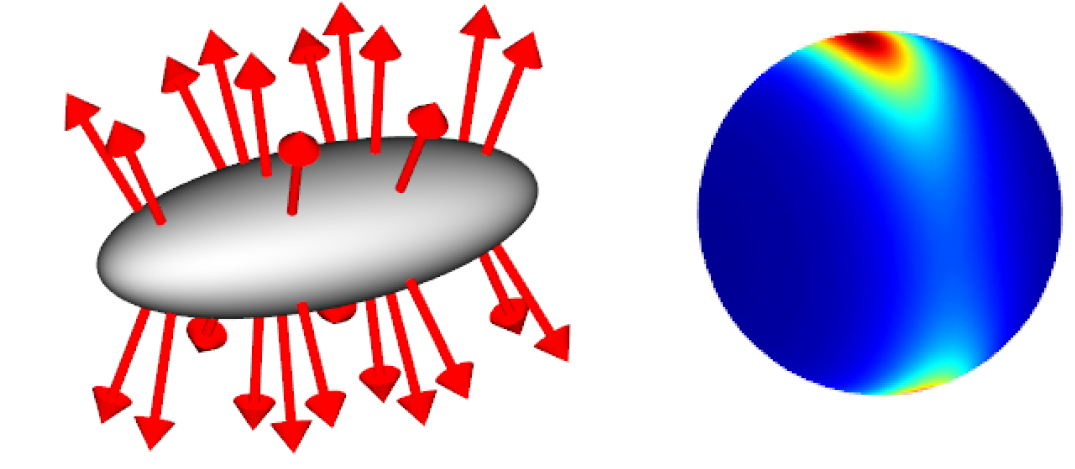
\includegraphics[width=1\linewidth]{img/sggx_ndf_b.jpg}
        \caption{SGGX $D(\omega_m), \omega_m \in \mathcal{S}^2$}
        \label{fig:sggx_ndf_b}
    \end{subfigure}
	\caption[Visualization of anisotropic \acsp{ndf}]{Visualization of anisotropic \acsp{ndf}. Note that the negative hemisphere of the SGGX \acs{ndf} is a mirroring of the positive hemisphere (Image from \cite{sggx}).}
	\label{fig:sggx_ndf}
\end{figure}
Based on the \acs{ndf} the authors then introduce a \ac{vndf} $D_{\omega_o}(\omega_m)$ which is used for importance sampling of the phase function, since it further reduces variance compared to the \acs{ndf} \cite{vndf_importance_sampling}.
Another important concept in the microflake framework is the projected area $\sigma(\omega_o)$ of the microflakes.
As depicted in Figure \ref{fig:sggx_projected_area}, this is the area of the microflakes when projected onto a plane in direction $\omega_o$ \cite{sggx}.
\begin{figure}[t]
    \centering
    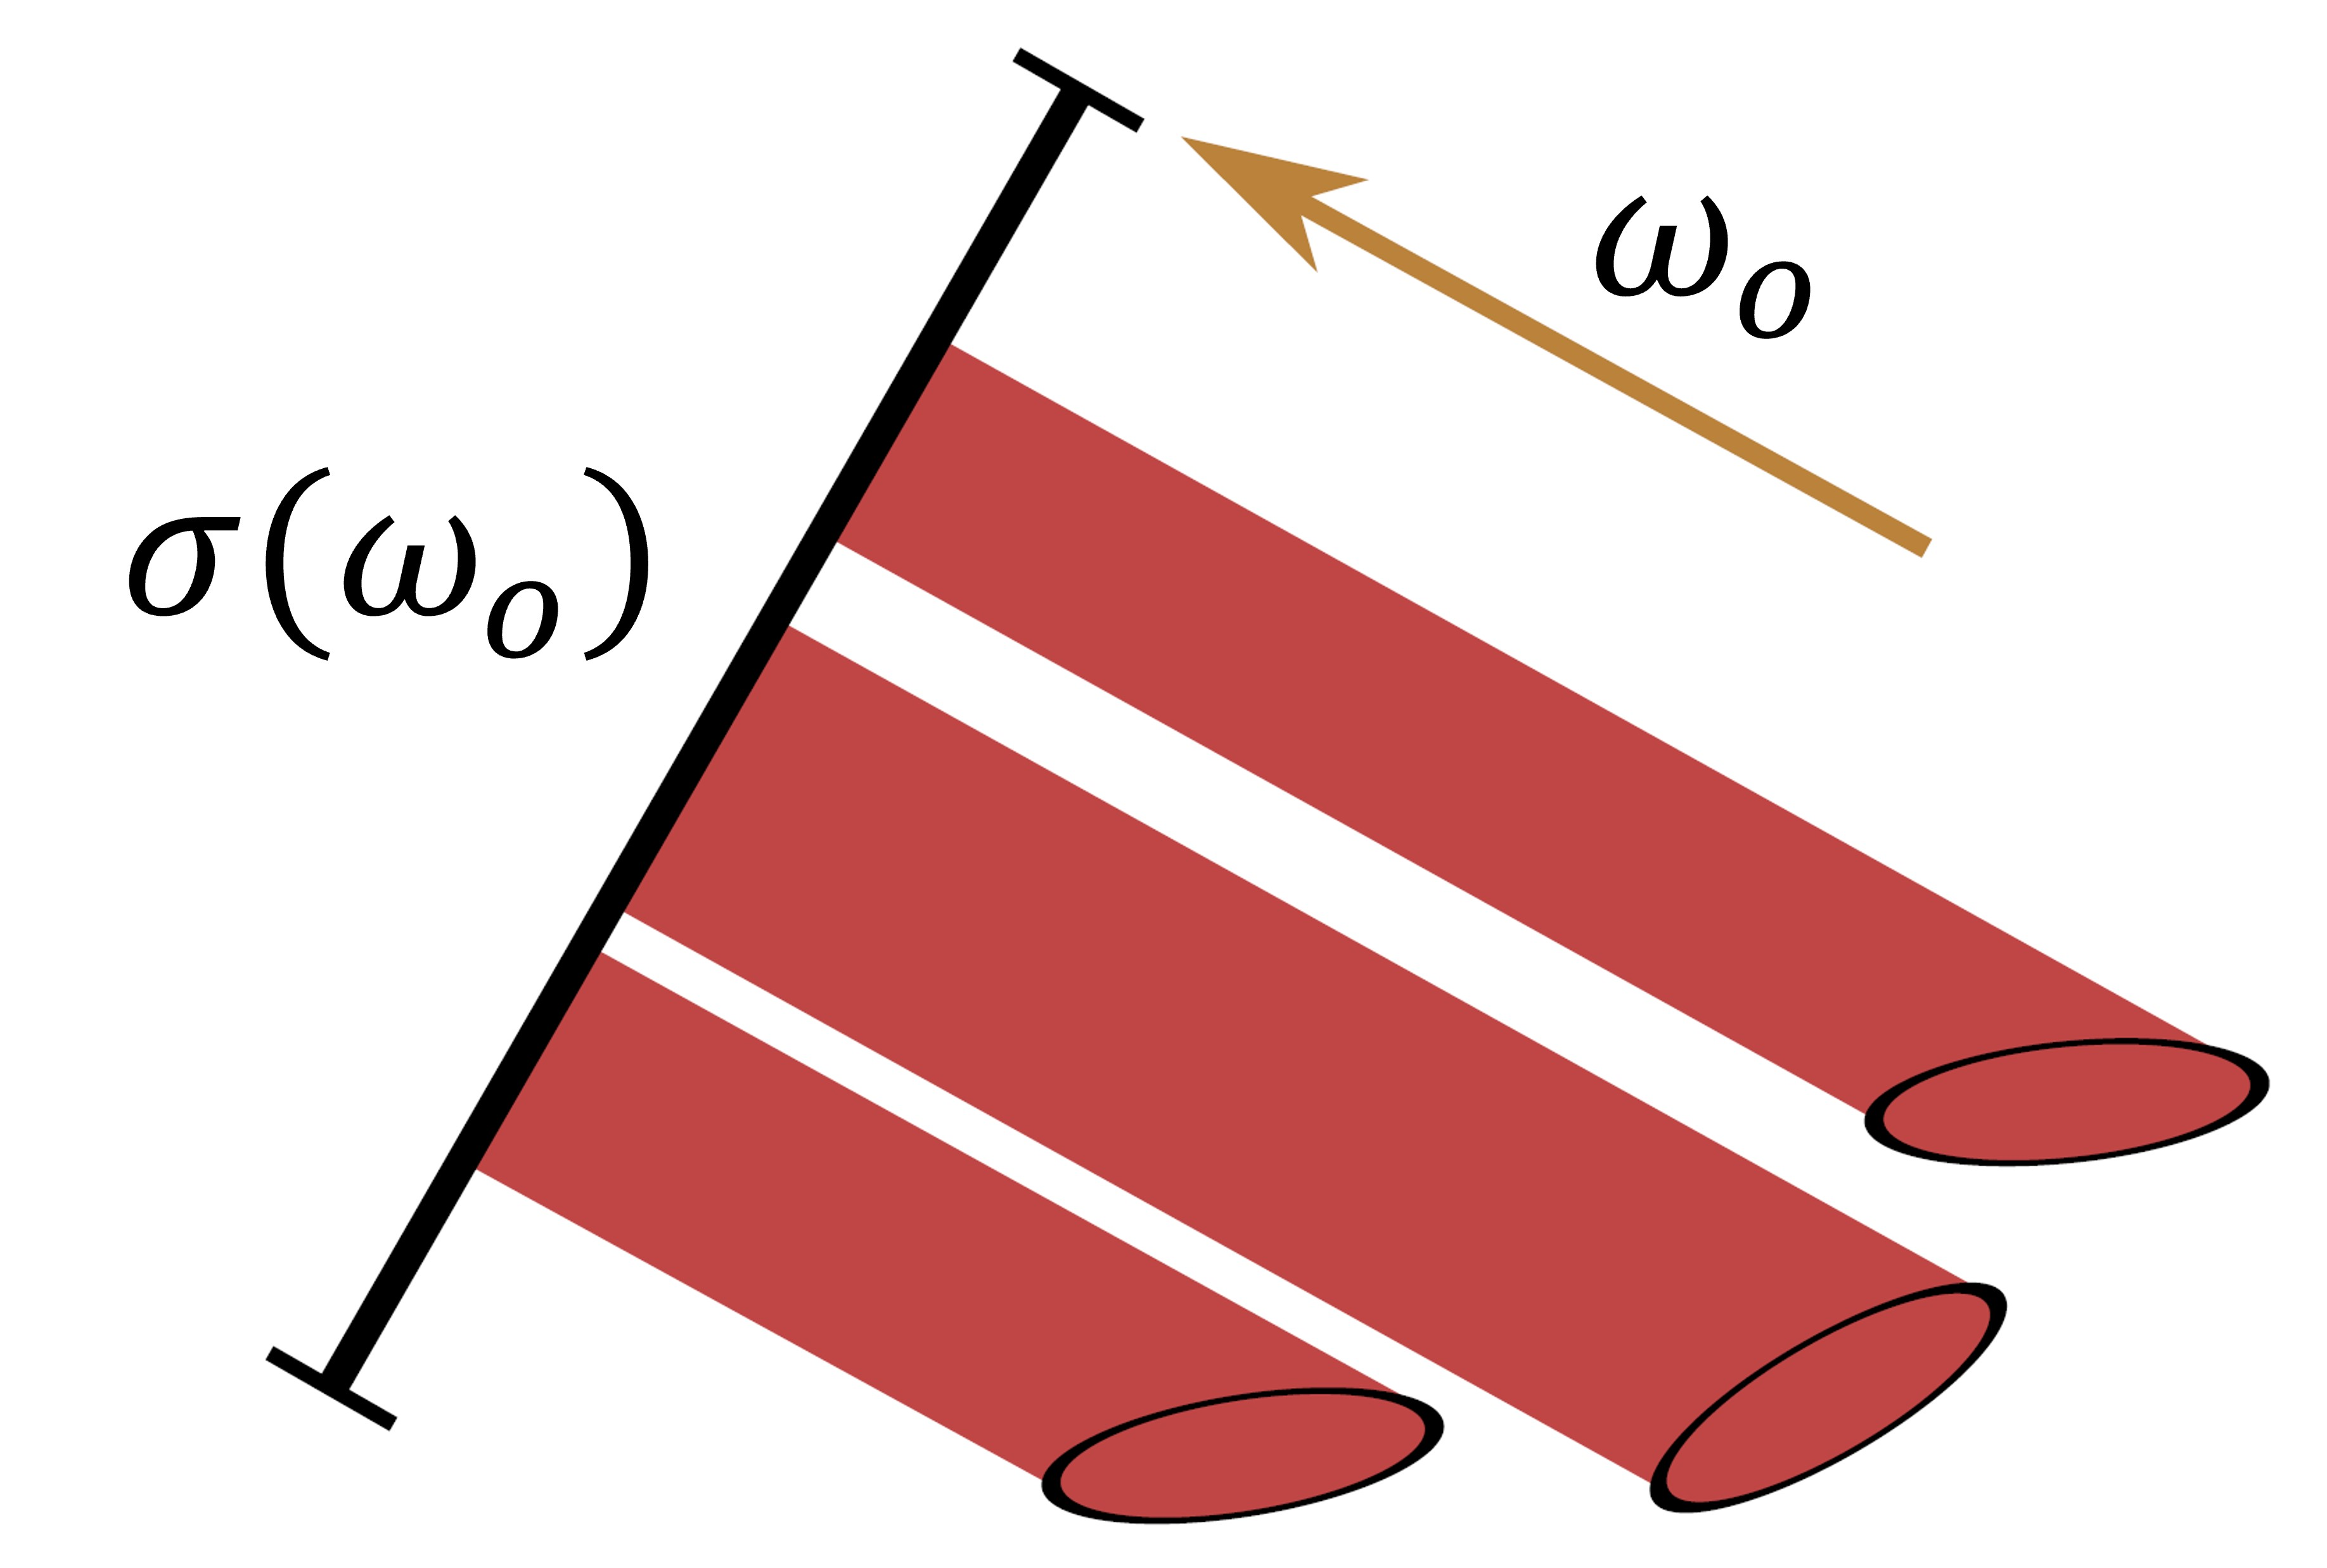
\includegraphics[width=0.3\linewidth]{img/sggx_projected_area.jpg}
    \caption[Illustration of the microflake projected area]{Illustration of the microflake projected area $\sigma(\omega_o)$, which is the area on a plane on which the microflakes are projected (Image from \cite{sggx}, with modification of the annotations).}
    \label{fig:sggx_projected_area}
\end{figure}
For the SGGX phase function the projected area is defined as:
\begin{equation}
    \label{eq:projected_area}
    \sigma(\omega_o)=\int_{\mathcal{S}^2} \langle \omega_o, \omega_m \rangle D(\omega_m) d\omega_m = \sqrt{\omega_o^T S \omega_o},
\end{equation}
where $\langle -,-\rangle$ denotes the clamped dot product \cite{sggx}.
Having defined these terms the authors introduce the actual phase function which consists of a specular and a diffuse component.
The specular component is evaluated as \cite{sggx}:
\begin{equation*}
    f{}^{spec}_p(\omega_o, \omega_i) = \frac{D(\omega_h)}{4 \sigma(\omega_o)}.
\end{equation*}
Importance sampling the specular component requires to sample a microflake normal $\omega_m$ from $D_{\omega_o}$ and the direction $\omega_o$ is reflected on this normal to generate an incident direction $\omega_i$ \cite{sggx}.
For evaluating the diffuse phase function the authors propose to sample a normal $\omega_m$ from $D_{w_o}$ which gives an unbiased estimate of the following integral \cite{sggx}:
\begin{equation*}
    f{}^{diff}_p(\omega_o, \omega_i) = \frac{1}{\pi}\int_{\mathcal{S}^2} \langle\omega_i,\omega_m\rangle D_{\omega_o}(\omega_m) d\omega_m = \lim \limits_{N \to +\infty} \frac{1}{N} \sum_{n=1}^N \frac{1}{\pi} \langle\omega_i,\omega_m(n)\rangle.
\end{equation*}
$f{}^{diff}_p$ can then be importance sampled by generating a direction $\omega_m$ from $D_{\omega_o}$ and then sampling the hemisphere given by $\omega_m$ \cite{sggx}.

\section{Transforming Meshes into Volumes}
\label{sec:transforming_meshes_into_volumes}
For generating \acp{lod} we need to transform the mesh representation into a volumetric representation.
We refer to this process as filtering.
% We follow the approach by \citeauthor{hybrid_mesh_volume_lods} and use ray casting to estimate the density for each voxel \cite{hybrid_mesh_volume_lods}.
We follow a similar approach as \citeauthor{hybrid_mesh_volume_lods} and use ray casting to estimate the density for each voxel \cite{hybrid_mesh_volume_lods}.
Our deviations from their approach are discussed in Section \ref{sec:mesh_filtering}.
To sample ray origins the authors use a \ac{pdf} $D_i=D_i^{cube} \ast D^{smooth}$ around the voxel center.
$D_i^{cube}$ is a cubic uniform \ac{pdf} around the center of voxel $i$ and $D^{smooth}$ is a 3D gaussian function with the standard deviation of 0.6 times the length of the voxel edge.
The length of the rays is set to the length of the voxel edge.
Each ray is intersected with the micro-geometry \cite{hybrid_mesh_volume_lods}.
The number of hits and the total number of rays casted determine the occlusion probability \cite{hybrid_mesh_volume_lods}:
\begin{equation*}
    P_{occ}=\frac{nbHits}{nbRays}.
\end{equation*}
Since a medium is defined on the density $\rho$ the authors solve the integral:
\begin{equation}
    1 - \frac{1}{4\pi}\int_{\mathcal{S}^2} e^{-\rho \, \sigma(\omega) \, ray_l} d\omega = P_{occ}
    \label{eq:loubet_filtering_equation}
\end{equation}
for $\rho$ \cite{hybrid_mesh_volume_lods}.
$\sigma_u(\omega)$ is the microflake projected area as defined in Equation \ref{eq:projected_area} and $ray_l$ is again the length of the voxel edge.
This equation cannot be solved analytically for the density and therefore requires gradient descent based optimization \cite{hybrid_mesh_volume_lods}.





 

\chapter{Method}
\label{chap:method}
For our experiments, we follow the steps depicted in Figure \ref{fig:pipeline}.
\begin{figure}[ht]
    \centering
    
\includegraphics[width=1.0\linewidth]{img/pipeline.png}
    % \includesvg[pretex=\tiny, width=1.0\linewidth]{img/pipeline}
    \caption[Visualization of the pipeline the thesis built upon]{Visualization of our pipeline for \ac{lod} generation. Yellow boxes represent files that are inputs our outputs of green program components. Evaluation is partially done by visual comparison and by computing image quality metrics.}
    \label{fig:pipeline}
\end{figure}
We first take the surface meshes and apply the filtering procedure to obtain the volume grids.
Additionally we save metadata like the bounding-box sizes of the grids, which we then need for scene generation.
This generation step can either generate ground-truth scenes that only contain meshes or it can generate scenes that use \acp{lod}.
The next step in the pipeline is the rendering of the scene, which uses mesh or volume files depending on the definitions in the generated scene file.
Finally we evaluate our results by comparing the mesh-only renderings with the ones that use \ac{lod}.
This is done regarding the image quality and the render performance between the mesh-only renderings and the \ac{lod} renderings.
We are however not interested in the absolute render times, but rather in the relative times between the mesh and volume representations.
This final evaluation step is explained in Chapter \ref{chap:results_and_discussion} while all other steps are subject of this chapter.

Although our pipeline can be used with arbitrary models, we only use tree models with it.
In total these are 26 free tree meshes from XfrogPlants \cite{xfrogplants} and the McGuire Computer Graphics Archive \cite{McGuire2017Data} which are available as \texttt{.obj} files with the textures being encoded as \texttt{.png} or \texttt{.tiff}.
Meshes and textures together occupy 1.2 GB of disk memory.
Apart from the models itself, XfrogPlants also provides information of the sizes the trees grow during their lifespan, which we also need during filtering and scene generation.

\section{Mesh filtering}
\label{sec:mesh_filtering}
As described in Section \ref{sec:transforming_meshes_into_volumes} we use the ray casting approach by \citeauthor{hybrid_mesh_volume_lods} with a few modifications for our filtering \cite{hybrid_mesh_volume_lods}.
The ray casting is \ac{gpu} accelerated using OptiX \cite{parker_optix}.
In contrast to \citeauthor{hybrid_mesh_volume_lods} we assume our particles to have an isotropic microflake projected area $\sigma$, meaning that it is not view dependent.
This greatly simplifies our optimization procedure as well as the distance sampling and transmittance estimation later during rendering.

During filtering we place the voxel grid over the mesh and align it to three sides of the bounding box of the mesh.
If the edge lengths of the mesh's bounding box do not evenly divide by the size of a voxel, we let the volume overlap on the non-aligned sides.
In each voxel we then sample the origin of our rays on a cubic uniform domain and the direction of the rays is uniformly sampled over the unit sphere.
\citeauthor{hybrid_mesh_volume_lods} use a ray length that is equal to the edge length of a voxel, which leads to a blurring since adjacent geometry is included in the density estimation.
As \citeauthor{wang_object_space_aliasing} points out, this can reduce object space aliasing \cite{wang_object_space_aliasing}.
However we think, that we can increase the spatial resolution while preserving the blurring by clipping the ray at a bounding sphere.
We position the sphere at the voxel's center and scale it so that its diameter is slightly larger than the diagonal of the voxel.
Each ray is then first intersected with this sphere to compute a $t_{max}$, before the intersection test with the mesh geometry happens.
Figure \ref{fig:raygen_filtering} compares our approach for determining the ray length with the approach of \citeauthor{hybrid_mesh_volume_lods}.
\begin{figure}[ht]
    \centering
    \begin{subfigure}[b]{0.25\linewidth}
        \centering
        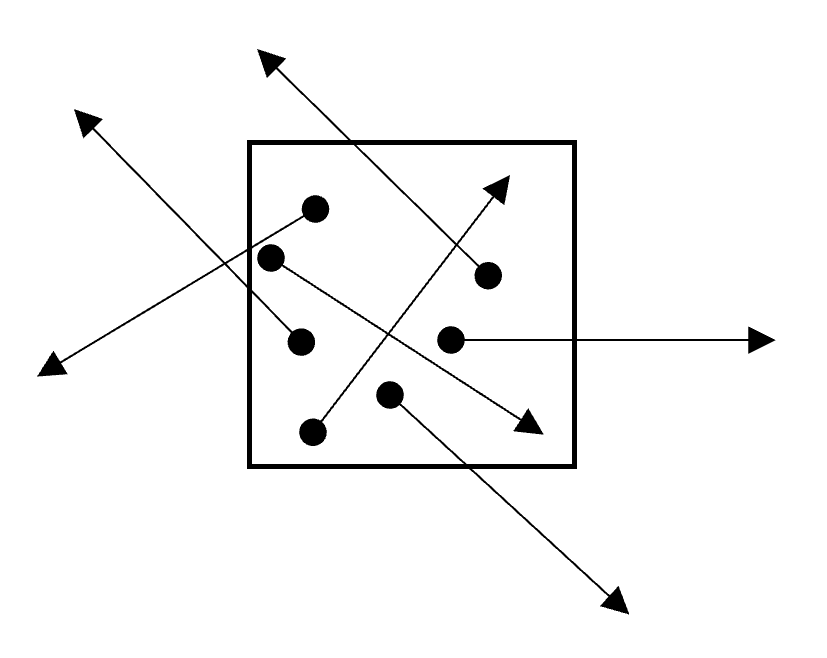
\includegraphics[width=\linewidth]{img/raygen_filtering_unclipped.png}
        \caption{}
        \label{fig:raygen_filtering_unclipped}
    \end{subfigure}
    \begin{subfigure}[b]{0.25\linewidth}
        \centering
        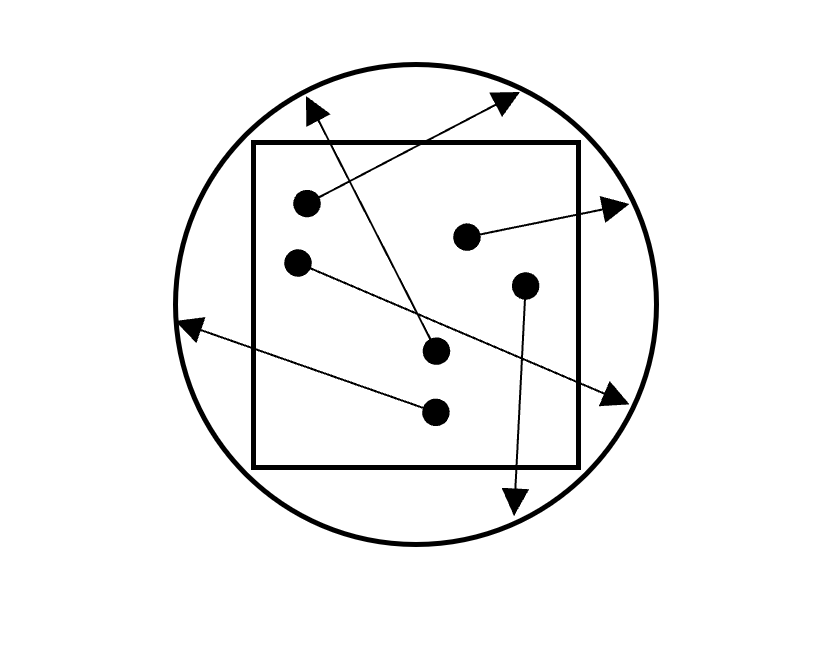
\includegraphics[width=1\linewidth]{img/raygen_filtering_clipped.png}
        \caption{}
        \label{fig:raygen_filtering_clipped}
    \end{subfigure}
	\caption[Approaches for determining a ray length for filtering]{Image (a) shows the approach by \citeauthor{hybrid_mesh_volume_lods} with constant ray length. Figure (b) shows our approach with ray clipping at a bounding sphere.}
	\label{fig:raygen_filtering}
\end{figure}

With these modifications we also have to solve a different integral than that from Equation \ref{eq:loubet_filtering_equation}.
We therefore have to find a density $\rho$ that suffices:
\begin{equation}
    1 - \frac{1}{4\pi}\int_{\mathcal{S}^2} e^{-\rho\sigma ray_l(\omega)} d\omega = P_{occ}.
    \label{eq:our_filtering_equation}
\end{equation}
Note that the projected area $\sigma$ is now independent of the direction $\omega$, whereas the ray length depends on $\omega$, since the rays are clipped by the bounding sphere.
As stated in Section \ref{sec:transforming_meshes_into_volumes}, we cannot solve for the density with analytical methods, therefore we iteratively optimize $rho$:
\begin{equation*}
    \rho_{i+1}=\rho_i - \alpha (P_{occ,volume} - P_{occ,mesh}),
\end{equation*}
where $i$ denotes the iteration, $\alpha$ is a learning rate, $P_{occ,mesh}$ is the ratio of geometry hits to the total number of rays casted and $P_{occ,volume}$ is the probability that a medium interaction takes place given the density $\rho$.
It is computed by Monte Carlo integrating Equation \ref{eq:our_filtering_equation}, so our estimator has the form:
\begin{equation*}
    1 - \frac{1}{N}\sum_{n=1}^{N} e^{-\rho\sigma ray_l(\omega_n)} = P_{occ,volume}.
\end{equation*}
Apart from this density estimate we also filter the diffuse and specular color of the geometry, the normals, the index of refraction and the SGGX Matrix $S$ by averaging.
The Matrix $S$ serves later as a coordinate frame for sampling reflection directions with the phase function \cite{sggx}.

% In total our attributes occupy 80 bytes of memory per voxel and we first represent them by a dense grid in the \ac{GPU}'s global memory.
We represent these attributes as a dense grid in the \acs{gpu}'s global memory.
OpenVDB cannot be used for this, because it is incompatible with CUDA device code \cite{museth_nanovdb}, NanoVDB on the other hand, is a read-only grid \cite{nanovdb}.
Only after copying the dense grid to host memory we convert it into an OpenVDB grid and subsequently into a NanoVDB grid which we store to disk.
Using NanoVDB however, imposes a limit of storing 32 bytes per voxel which we can't increase in the limited time frame of the thesis \cite{open_to_nanovdb}.
Because our attributes occupy 80 bytes of memory, we use quantization to represent the values in the grid and before doing computations like interpolation or shading, we transform them back to the full width.
The following table summarizes the size of all attributes in regular and quantized format (ignoring padding):
\begin{center}
    \begin{tabular}{| c | c | c | }
        \hline
         & Regular Format & Quantized Format \\
         \hline
         Density & $1\times 4\;\text{bytes}$ & $1\times 4\;\text{bytes}$ \\
         \hline
         $S$ & $9\times 4\;\text{bytes}$ & $6\times 2\;\text{bytes}$ \\
         \hline
         Diffuse color & $3\times 4\;\text{bytes}$ & $3\times 1\;\text{bytes}$ \\
         \hline
         Specular color & $3\times 4\;\text{bytes}$ & $3\times 1\;\text{bytes}$ \\
         \hline
         Normal & $3\times 4\;\text{bytes}$ & $3\times 2\;\text{bytes}$ \\
         \hline
         Index of refraction & $1\times 4\;\text{bytes}$ & $1\times 2\;\text{bytes}$ \\
         \thickhline
         Total & $80\;\text{bytes}$ & $30\;\text{bytes}$ \\
         \hline
    \end{tabular}
\end{center}
Note that since $S$ is a symmetric matrix, it is enough to store six coefficients \cite{sggx}.
Apart from storing the NanoVDB grid we also store the brick grid, which only contains the density values of each voxel.
In principle, it would be possible to store all voxel attributes in brick grid, though the performance gain would be small and modifying brick grid to support this would take some time.
For every \ac{lod} we also export metadata which encompasses the number of voxels in the grid and the bounding box dimensions during filtering.

We generate 7 \acsp{lod} for voxel sizes from 0.1m to 6.4m, doubling the size of a voxel for each \ac{lod}.
The number of voxels is then computed from the voxel size and the size of the trees.
The reason for choosing a voxel size between 0.1m and 6.4m is because for finer voxels the grids quickly use more memory than their surface representations while choosing even larger sizes has no effect, since some trees are already represented by a single voxel on the coarsest level.
The resulting grids occupy 940MB of disk space, where the finest \acsp{lod} are responsible for 65\% of this data.
In chapter \ref{chap:results_and_discussion} we discuss how dropping this \ac{lod} affects image quality and rendering times.

Having the \acsp{lod}, Figure \ref{fig:lods_comparison} compares them to the surface representation for some models.
\begin{figure}[ht]
    \begin{center}
        \begin{tabularx}{\textwidth}{ X  X  X  X  }
            \hline
            Model & Mesh & Volume \newline(Voxel size = 0.1m) & Volume \newline(Voxel size = 0.8m) \\
            \hline
            Acer\newline rubrum\newline adult & \adjustimage{height=3.9cm,valign=m}{img/EA01a_mesh.png} & \adjustimage{height=3.9cm,valign=m}{img/EA01a_0.1.png} & \adjustimage{height=3.9cm,valign=m}{img/EA01a_0.8.png} \\
            \hline
            Acacia\newline sophorae 9 & \adjustimage{height=3.9cm,valign=m}{img/OC41_9_mesh.png} & \adjustimage{height=3.9cm,valign=m}{img/OC41_9_0.1.png} & \adjustimage{height=3.9cm,valign=m}{img/OC41_9_0.8.png} \\
            \hline
            Celtis\newline australis\newline medium & \adjustimage{height=3.9cm,valign=m}{img/EU06m_mesh.png} & \adjustimage{height=3.9cm,valign=m}{img/EU06m_0.1.png} & \adjustimage{height=3.9cm,valign=m}{img/EU06m_0.8.png} \\
            \hline
            Pinus\newline muricata\newline adult & \adjustimage{height=3.9cm,valign=m}{img/CL13a_mesh.png} & \adjustimage{height=3.9cm,valign=m}{img/CL13a_0.1.png} & \adjustimage{height=3.9cm,valign=m}{img/CL13a_0.8.png} \\
            \hline
        \end{tabularx}
    \end{center}
    \caption[Comparison between mesh and volume renderings]{Comparison between the surface representation in the first column and two different \acsp{lod} in columns two and three.}
    \label{fig:lods_comparison}
\end{figure}

\section{Scene Generation}
\label{sec:scene_generation}
We implement the scene generator in Python.
It uses the volume metadata that is exported during filtering and generates a circular forest with uniformly distributed trees.
Our generator uses a rejection sampling approach, rejecting samples that are too close to another.
It is therefore similar to a poisson disk sampler \cite{poisson_sampling}, however it uses varying spacing between the samples depending on the model size.
This is why we exported the bounding box sizes of the volumes during filtering.
First we identify the largest bounding box for each model.
Differences in the bounding box size of a model can occur, because during filtering we make sure that the mesh is fully enclosed by voxels for a given voxel size.
This effect is visualized in Figure \ref{fig:bounding_sizes}.
\begin{figure}[ht]
    \centering
    \begin{subfigure}[b]{0.45\linewidth}
        \centering
        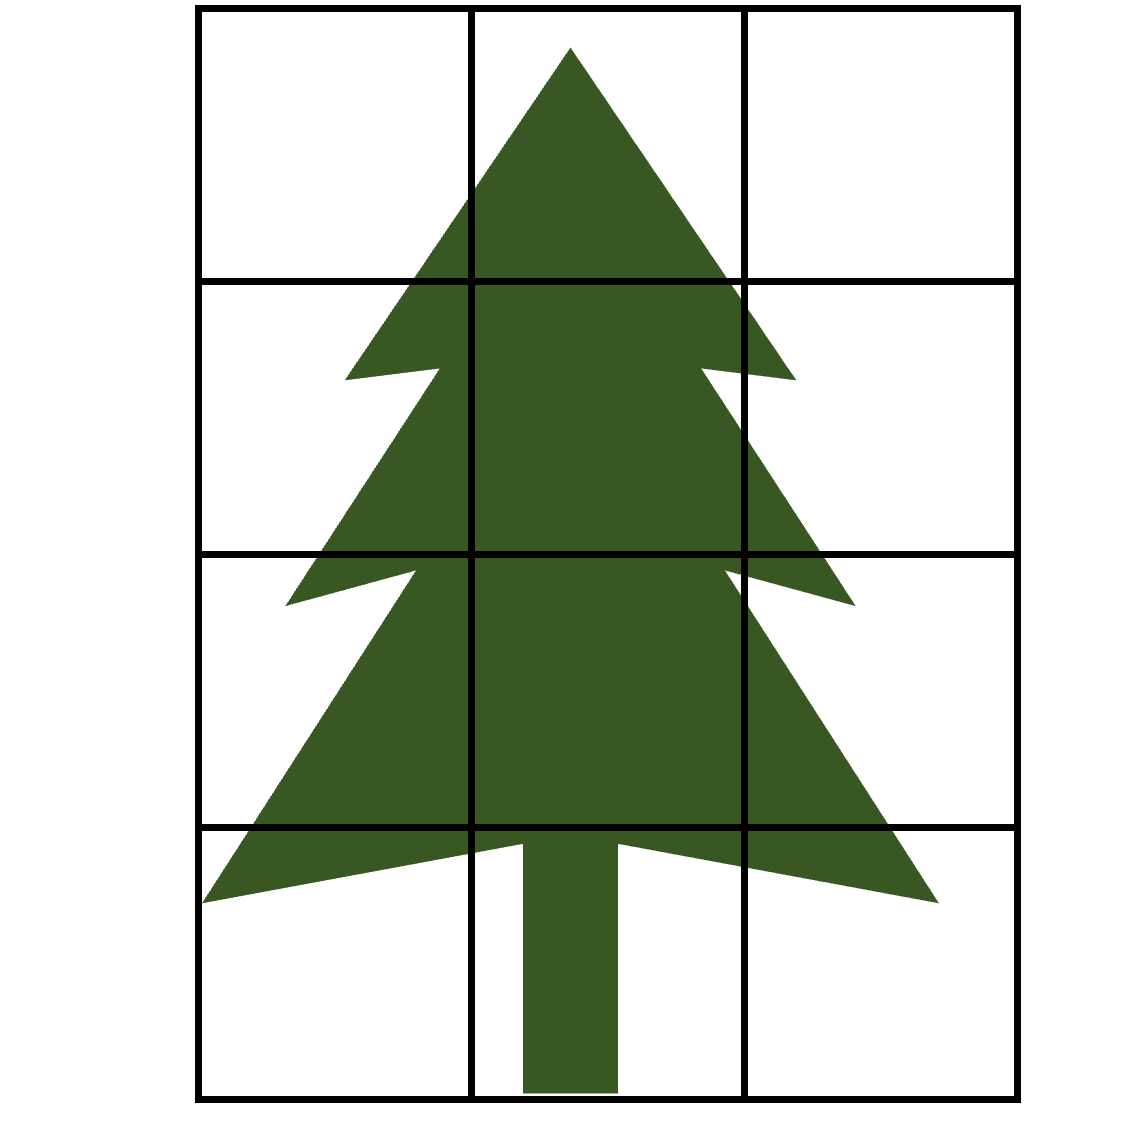
\includegraphics[height=4cm]{img/bounding_size_1.png}
        % \caption{}
        % \label{fig:bounding_size_1}
    \end{subfigure}
    \begin{subfigure}[b]{0.45\linewidth}
        \centering
        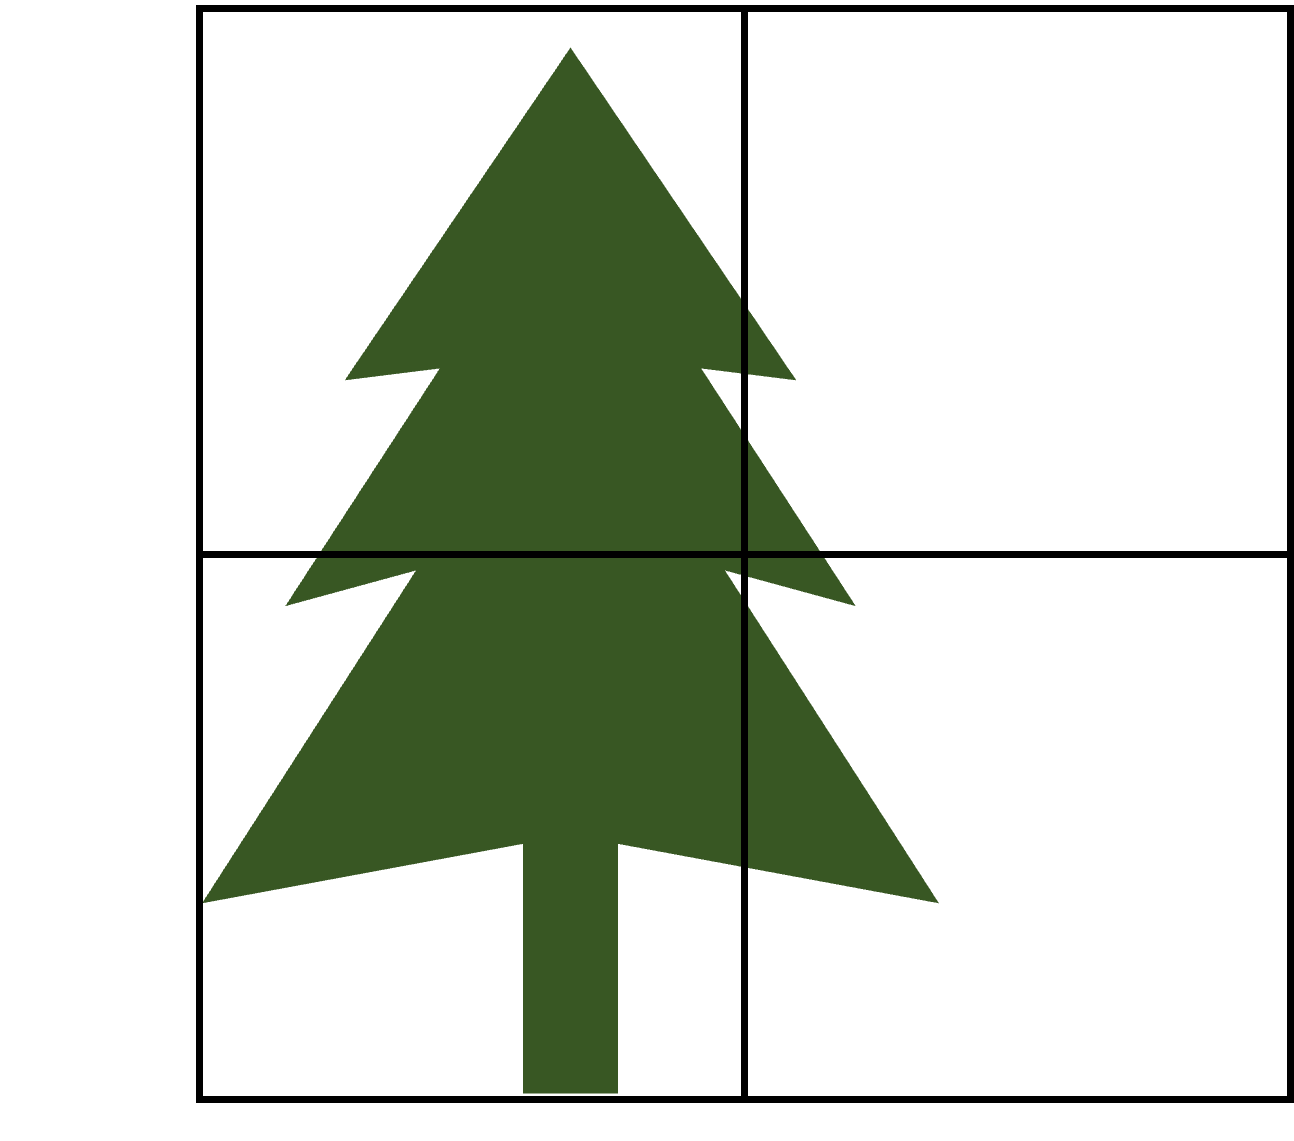
\includegraphics[height=4cm]{img/bounding_size_2.png}
        % \caption{}
        % \label{fig:bounding_size_2}
    \end{subfigure}
	\caption[Bounding boxes resulting from different sized voxels]{The volume is always aligned to one side of the mesh. If we have different sized voxels (like \acsp{lod} necessarily have) the volume overlaps on one side and the bounding box sizes differ.}
	\label{fig:bounding_sizes}
\end{figure}
Then we sample a class \textit{Large}, \textit{Medium}, \textit{Small}, which contain tree models in the corresponding sizes.
We assign trees that grow 20-35 meters to the class \textit{Large}, trees that reach 10-20 meters are labeled as \textit{Medium} and trees that are smaller than 10 meters are assigned to the \textit{Small} class.
This allows us to control the age of the forest.
For example, if we want an old forest we increase the probability for class \textit{Large} and if we want a rather young forest we increase the probability for \textit{Small} trees.
We then choose a tree from this class, sample a position in the circle and check whether it collides with existing models.
This step is a significant performance bottleneck for all rejection based sampling procedures.
In our case we need 100000 sample positions to generate a scene with only 9924 trees.
For all of these sampled positions we have to test whether the models overlap.
In order to accelerate this we employ a spatial acceleration structure: Since our forest has circular shape, we subdivide this circle into concentric segments.
We then have to check for a collision only in the segments in which our model is located.
The collision test itself is based on cylinders around the bounding boxes of the models, which may not overlap.
This acceleration reduces the scene generation with our Python script to a managable runtime of 6 minutes.

Having successively sampled an empty place in the circular forest we still get an overlap if we place a model at this exact position.
The reason is that the bounding box of the model might be asymmetrical.
For example: Consider a bounding box $BB_{min}=(-2.5, -5.0)$, $BB_{max}=(6.0, 10.0)$ and a sampled location $Pos_{center}=(1.5, 3.0)$.
The sampled location gives us the position where the \textit{center} of the bounding box namely $BB_{center}=(1.75, 2.5)$ has to be located.
However, all transformation matrices we use operate on the \textit{origin} of the model space.
Thus we have to compute the position of the origin in world space using:
\begin{equation*}
    Pos_{origin}=\frac{2Pos_{center}-Scale(BB_{min}+BB_{max})}{2},
\end{equation*}
where $Scale$ is an additional scaling factor for controlling the size of the model.
In our example, assuming a scaling of 1, this gives a location for the model of $Pos_{origin}=(-0.25, 0.5)$.

If we generate a ground truth scene, meaning that it contains only mesh models, we can now add the model to the scene, else we now have to determine the appropriate \ac{lod} for the model given the distance to the camera.
Knowledge of the camera position, gaze direction, the \ac{fov} and the sensor resolution are essential for that.
Note that a consequence is, that this information is baked into the scene description and moving the camera during rendering leads to a mismatch of the \acp{lod}.
Generating the scene in the renderer on the fly is currently no option, since this would lead to significantly worse performance of the renderer.
For positions outside the view frustum, we choose the coarsest \ac{lod} since these are not visible and only participate in indirect lighting.
If the position is inside the view frustum, we project the eight bounding box vertices of the coarsest volume on the image plane and compute the area of their convex hull using \texttt{scipy.spatial.ConvexHull} \cite{scipy}.
This gives us the number of pixels that the volume covers on the sensor.
We want to select \acp{lod} based on the heuristic that each voxel covers at most one pixel:
\begin{equation*}
    \frac{n_{voxel}}{n_{pixel}} > 1.
\end{equation*}
Therefore, we now have to compute the number of voxels that we see.
Calculating the product of the number of voxels in depth, height and width gives too many voxels, since some of the voxels are hidden by others.
Computing $depth \times height$, $depth \times width$ or $height \times width$ is only valid for viewing angles that are perpendicular to the surface of the voxel grid.
Another approach is to position a plane at the center of the grid and orient it towards the camera.
The number of voxels that this plane intersects would then be a ground truth value for the voxels that we see.
Evaluating this however, is really expensive since each voxel has to be tested whether it intersects the plane.
We choose a faster approach that approximates this value and is depicted in Figure \ref{fig:voxel_estimation}.
\begin{figure}[ht]
    \centering
    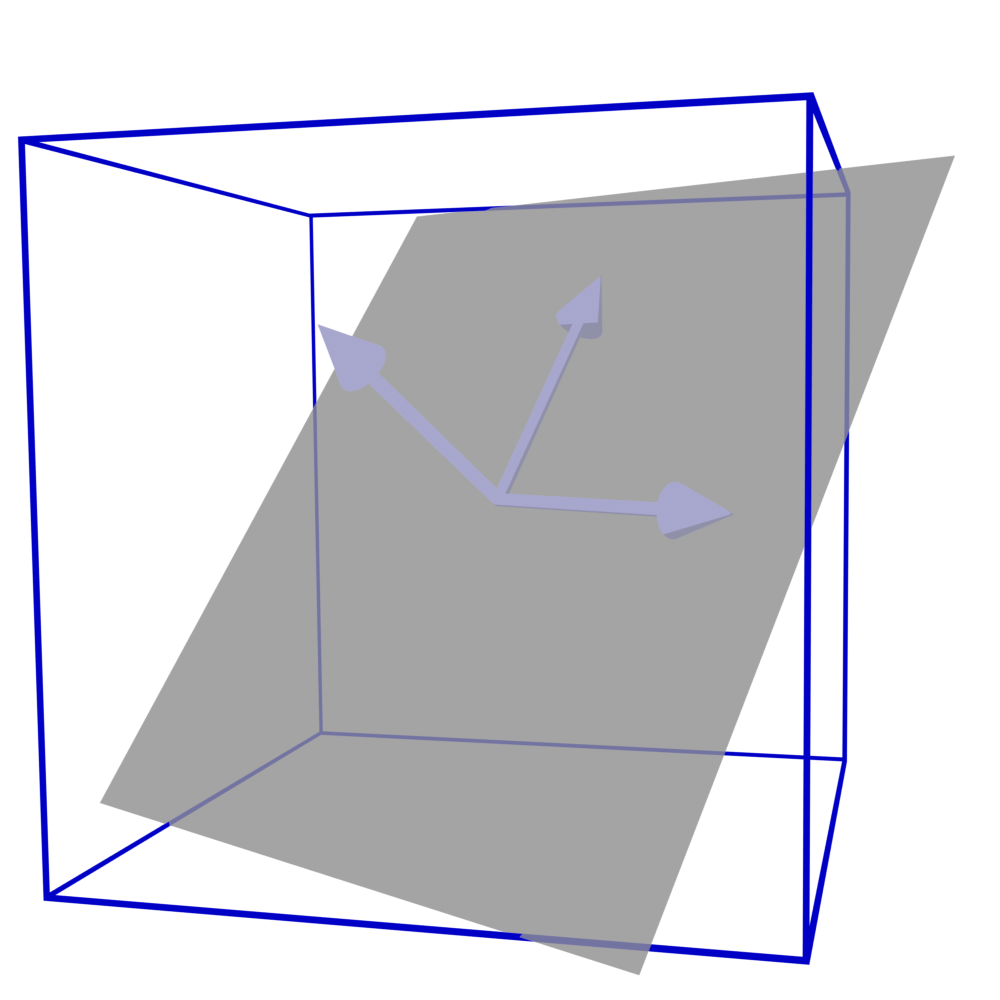
\includegraphics[width=0.3\linewidth]{img/voxel_estimation.png}
    % \includesvg[pretex=\tiny, width=1.0\linewidth]{img/pipeline}
    \caption[Estimation of intersected voxels]{We estimate the number of intersected voxels by shooting two rays which are perpendicular to the camera direction (plane normal). After intersecting them with the bounding box we can construct a rectangle whose area approximates the number of voxels intersected by a plane. The true value is different, since a plane intersecting a cube can produce anything from a triangular to a hexagonal area.}
    \label{fig:voxel_estimation}
\end{figure}
From the center of the volume bounding box we shoot a ray perpendicular to the camera direction horizontally.
A second ray is shot in a direction perpendicular to the first ray and perpendicular to the direction towards the camera.
We intersect the rays with the bounding box which gives us the number of voxels they passed.
By multiplying the results from both rays we get the number of voxels a rectangle located at the bounding box center intersects.
The ground truth value for the number of intersected voxels by a plane can be different, since a plane intersecting a cube does not necessarily give a rectangle.
However we found that our approach closely approximates the true value.
Having computed the number of voxels we can now choose the coarsest \ac{lod} that still fulfills our heuristic and add it to our scene.

As written before we repeat this procedure 100000 times to get a scene with 9924 trees, which are distributed over a circular area with a radius of 1000 meters.
Figure \ref{fig:visualize_lods} shows this scene rendered from the top with colored bounding boxes of the volumes.
\begin{figure}[ht]
    \centering
    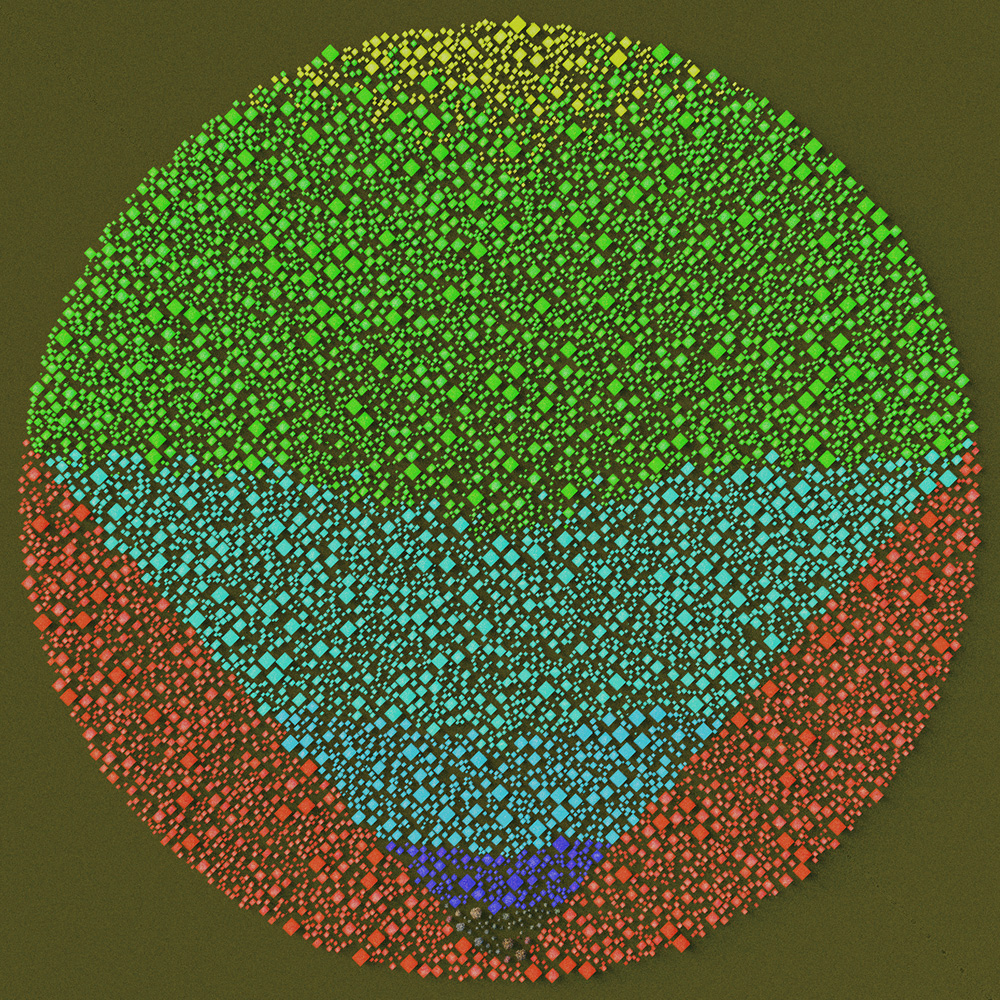
\includegraphics[width=0.5\linewidth]{img/visualize_lods.jpg}
    % \includesvg[pretex=\tiny, width=1.0\linewidth]{img/pipeline}
    \caption[Visualization of a \ac{lod} scene]{Visualization of a debug view of the generated scene using our heuristic. The different voxel sizes between each \ac{lod} are visualized by different colors of the bounding boxes. The colors range from blue, which represents the finest \ac{lod} with a voxel size of $\SI{0.1}{m}$, to red which represents the \acsp{lod} with a voxel size of $\SI{6.4}{m}$.}
    \label{fig:visualize_lods}
\end{figure}
It is clearly visible that we start rendering with meshes and then switch to successively coarser \acsp{lod} with further distance from the camera.
Additionally we see the frustum of the camera: Within the view frustum we select between different \acsp{lod} while we simply choose the coarsest \ac{lod} with a voxel size of 6.4 meters outside the frustum.


\section{Rendering}
\label{sec:rendering}
We render meshes and volumes using path tracing.
Like our filtering implementation, our path-tracer is also \ac{gpu} accelerated using OptiX \cite{parker_optix}.
For fast convergence we employ next event estimation and use importance sampling of the scattering functions and the environment map.
Russian roulette is used to terminate insignificant paths.
In order to render scenes with many meshes and volumes, we use instancing.
A certain mesh or volume thus has to occupy \ac{gpu} memory just once and for each usage an instance is created, each with its own model transformation.
We do the same for textures, loading only textures that differ in their file path.
Each material then stores a pointer to the memory location of the texture.

Our surfaces use the lambertian diffuse \cite{lambert} and the Trowbridge-Reitz microfacet \ac{brdf} \cite{trowbridge_reitz}, which is the general form of the GGX \ac{brdf}.
As Figure \ref{fig:leaf_gloss} shows, real leafs can have a specular gloss, therefore we incorporate a specular \ac{brdf}.
\begin{figure}[ht]
    \centering
    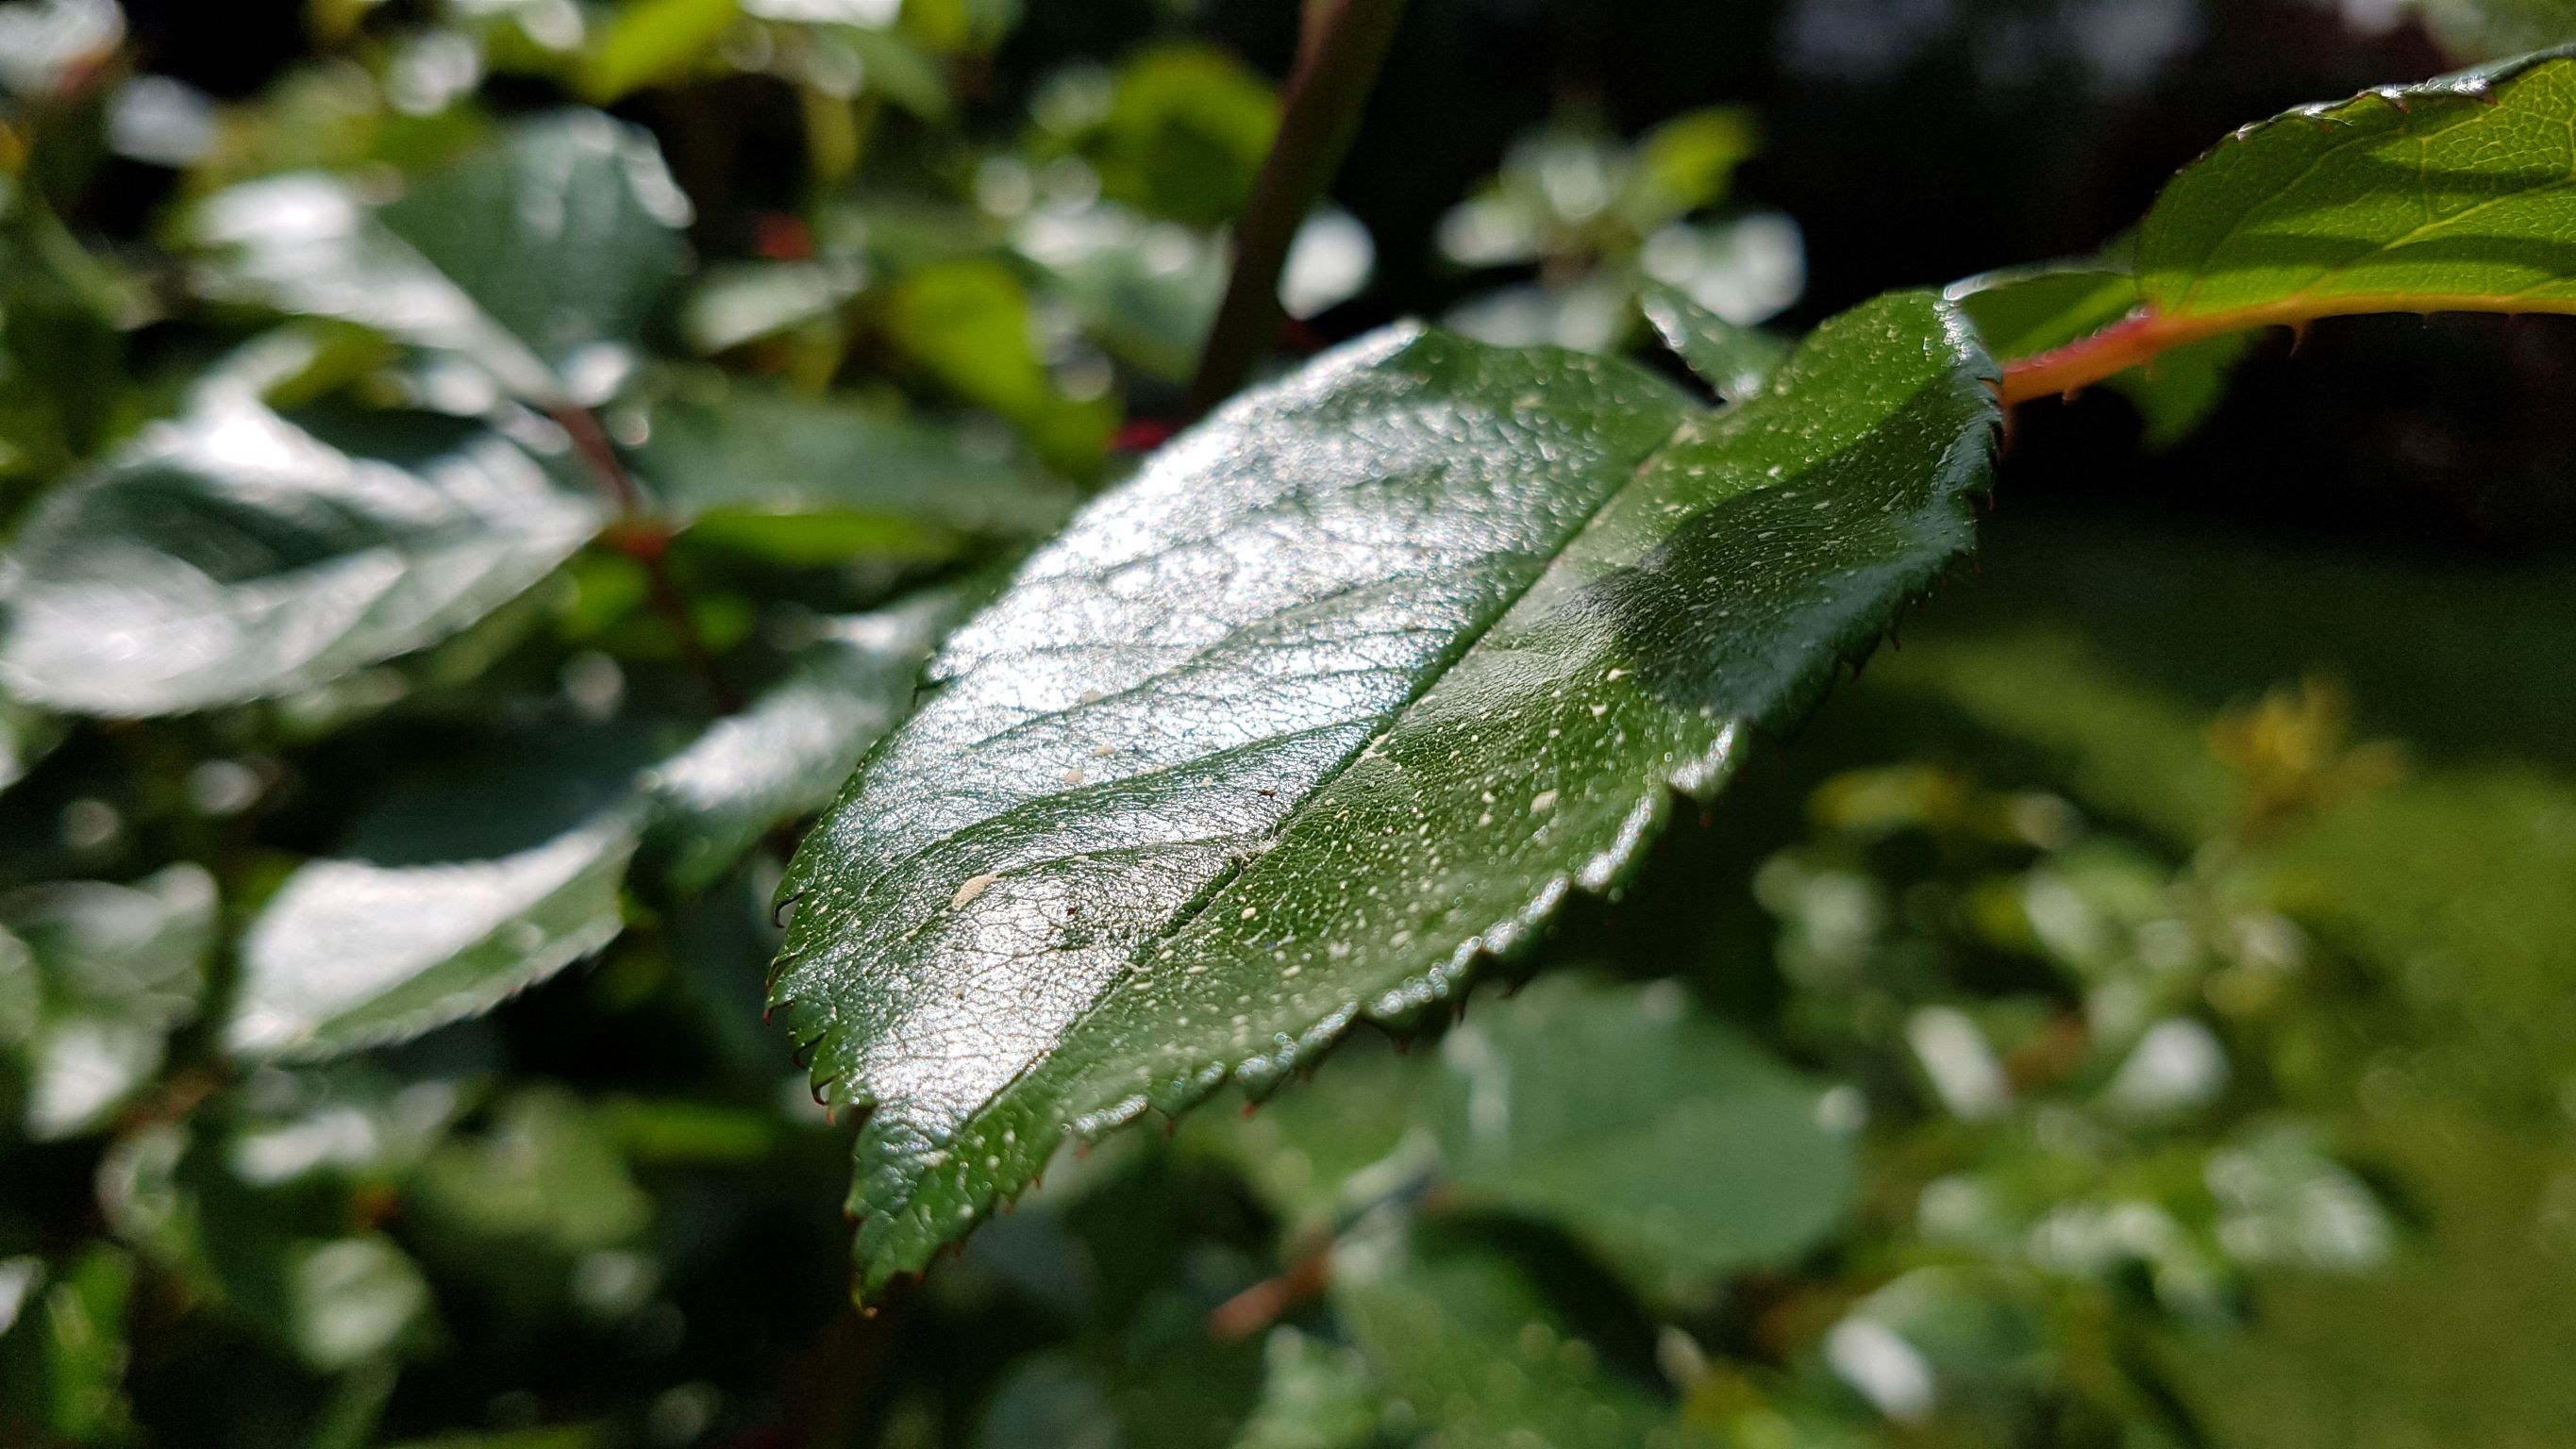
\includegraphics[width=0.5\linewidth]{img/leaf_gloss.jpg}
    % \includesvg[pretex=\tiny, width=1.0\linewidth]{img/pipeline}
    \caption[Leaf with glossy surface]{Real leafs often have a specular reflecting layer, therefore we incorporate a specular \ac{brdf} in our lighting calculations.}
    \label{fig:leaf_gloss}
\end{figure} 
The models we use neither have a specular map nor a specular color associated in their materials.
In order to still achieve the desired look it is possible to simply set the specular color to white, leading to a loss of structural information in the highlights.
Using the diffuse texture directly as a specular map results in colored highlights which does not match Figure \ref{fig:leaf_gloss}.
Therefore we first compute the luminosity of the diffuse texture which we then use as a specular map.
Figure \ref{fig:leaf_renderings} shows renderings of this approach.
\begin{figure}[ht]
    \centering
    \begin{subfigure}[b]{0.3\linewidth}
        \centering
        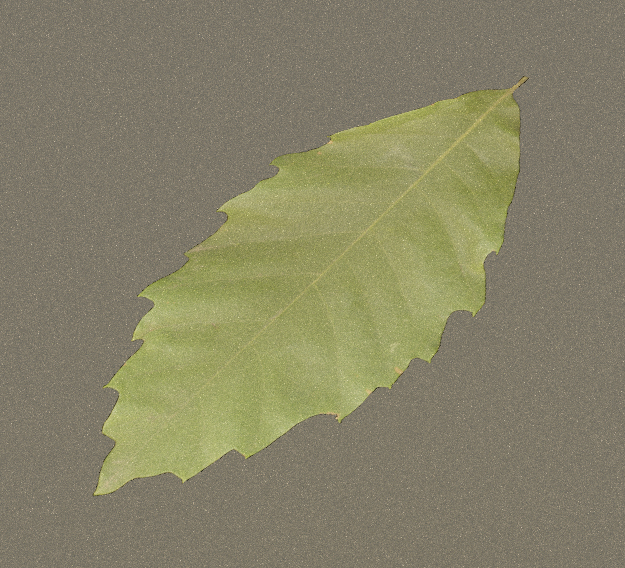
\includegraphics[width=1\linewidth]{img/leaf_no_spec.jpg}
        \caption{}
        % \label{fig:bounding_size_1}
    \end{subfigure}
    \begin{subfigure}[b]{0.3\linewidth}
        \centering
        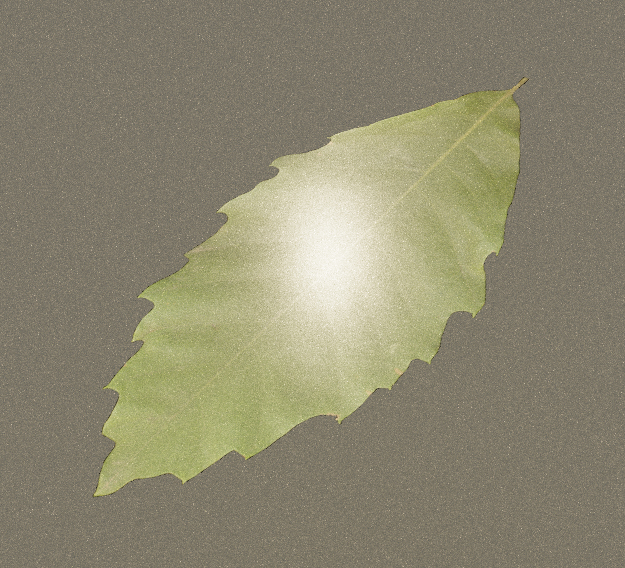
\includegraphics[width=1\linewidth]{img/leaf_spec.jpg}
        \caption{}
        % \label{fig:bounding_size_2}
    \end{subfigure}
	\caption[Comparison of renderings with and without specular maps]{Renderings of leafs using the default material (a) and our modification of converting the diffuse texture to a specular map (b).}
	\label{fig:leaf_renderings}
\end{figure}
We combine the diffuse and microfacet \ac{brdf} using the Fresnel term $F$ \cite{fresnel}, which describes the amount of light reflected on a surface.
It evaluates to values close to one for grazing angles and to one when light hits the surface perpendicularly \cite{pbr}.
For a layered surface the effect of the diffuse reflection is biggest near perpendicular angles while specular reflection mostly is visible near grazing angles \cite{pbr}.
We can therefore write our combined \ac{brdf} as:
\begin{equation*}
    f(\boldsymbol{x}, \omega_o, \omega_i) = F(|n_{\boldsymbol{x}} \cdot \omega_o|)f_{spec}(\boldsymbol{x}, \omega_o, \omega_i) + (1 - F(|n_{\boldsymbol{x}} \cdot \omega_o|))f_{diff}(\boldsymbol{x}, \omega_o, \omega_i).
\end{equation*}

As described in Section \ref{subsec:solving_beer_lambert_law_in_heterogeneous_media}, we use brick grid by \citeauthor{brick_grid} \cite{brick_grid} to represent the density values of a volume.
The authors also provide an implementation of the distance sampling procedure they use \cite{brick_grid}, which we rougly follow.
We use their distance sampling until we find an interaction and then perform a lookup in the NanoVDB grid to retrieve a filtered normal, diffuse and specular color, the index of refraction and the \ac{sggx} matrix $S$.
Since our procedure returns the albedo at this point of the medium, we now have to compute which frequencies of the light are absorbed, which is given by the color.
Just as for our surface rendering we apply the Fresnel term to weight the diffuse and specular color.
Because the Fresnel term requires a surface normal, we now use the filtered normal that we also stored in the NanoVDB grid.
We weight the specular color by $F$ and the diffuse color by $1-F$ to obtain our albedo.

At each sampled interaction in the medium we sample a new ray direction using the \ac{sggx} phase function.
Again we use the Fresnel term, this time to get a probability whether we should sample the diffuse phase function or the specular phase function.
Both phase functions rely on sampling a microflake normal from the \ac{sggx} \acl{vndf}.
% In contrast to \citeauthor{sggx} \cite{sggx}, we do not align this microflake normal with the ray direction $\omega_o$, but with the filtered normal $n$.
In contrast to \citeauthor{sggx} \cite{sggx}, we do not build a coordinate frame around the ray direction $\omega_o$, but we build it around the filtered normal $n$ to transform the microflake normal to world space.
Figure \ref{fig:tree_normal_maps} illustrates the normals of the mesh in world space and when the microflake normal is transformed with a coordinate frame around the direction $\omega_o$ or the filtered normal.
\begin{figure}[ht]
    \centering
    \begin{subfigure}[b]{0.3\linewidth}
        \centering
        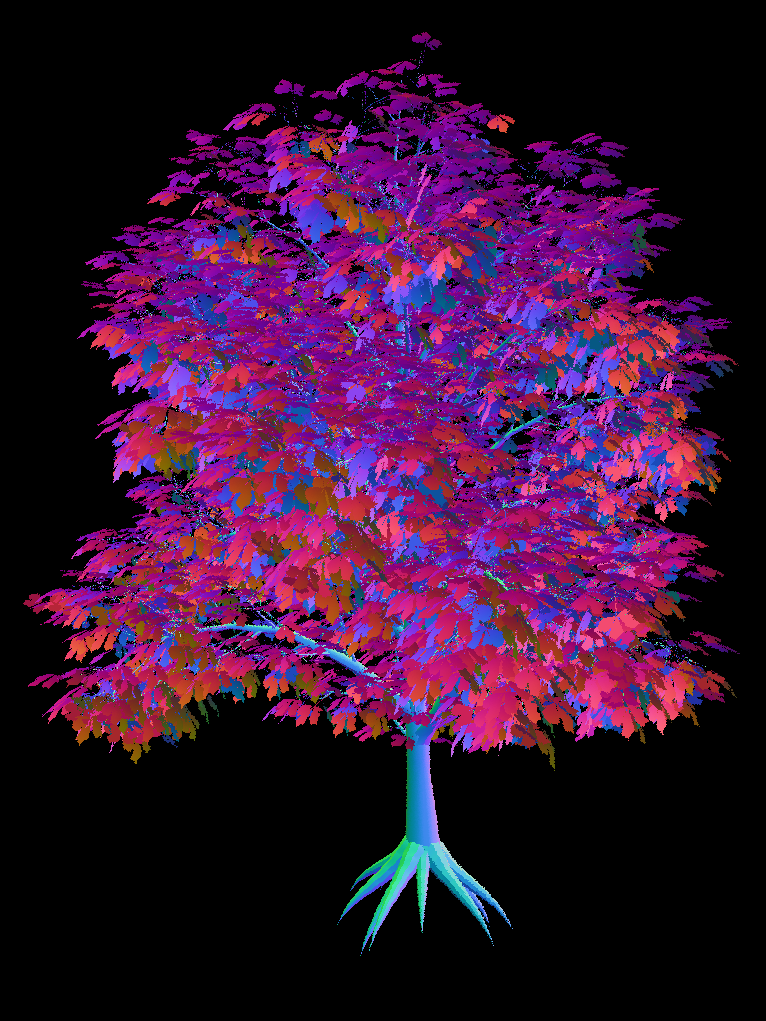
\includegraphics[width=1\linewidth]{img/normal_map_mesh.png}
        \caption{}
        % \label{fig:bounding_size_1}
    \end{subfigure}
    \begin{subfigure}[b]{0.3\linewidth}
        \centering
        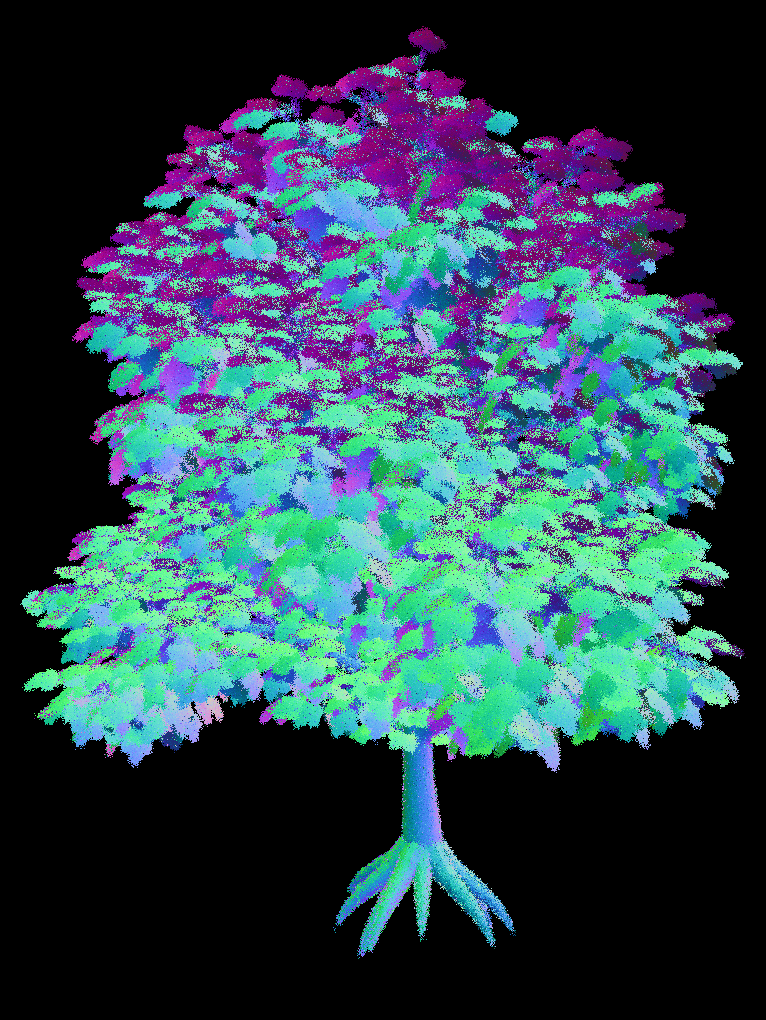
\includegraphics[width=1\linewidth]{img/normal_map_vndf_wo_aligned.png}
        \caption{}
        % \label{fig:bounding_size_2}
    \end{subfigure}
    \begin{subfigure}[b]{0.3\linewidth}
        \centering
        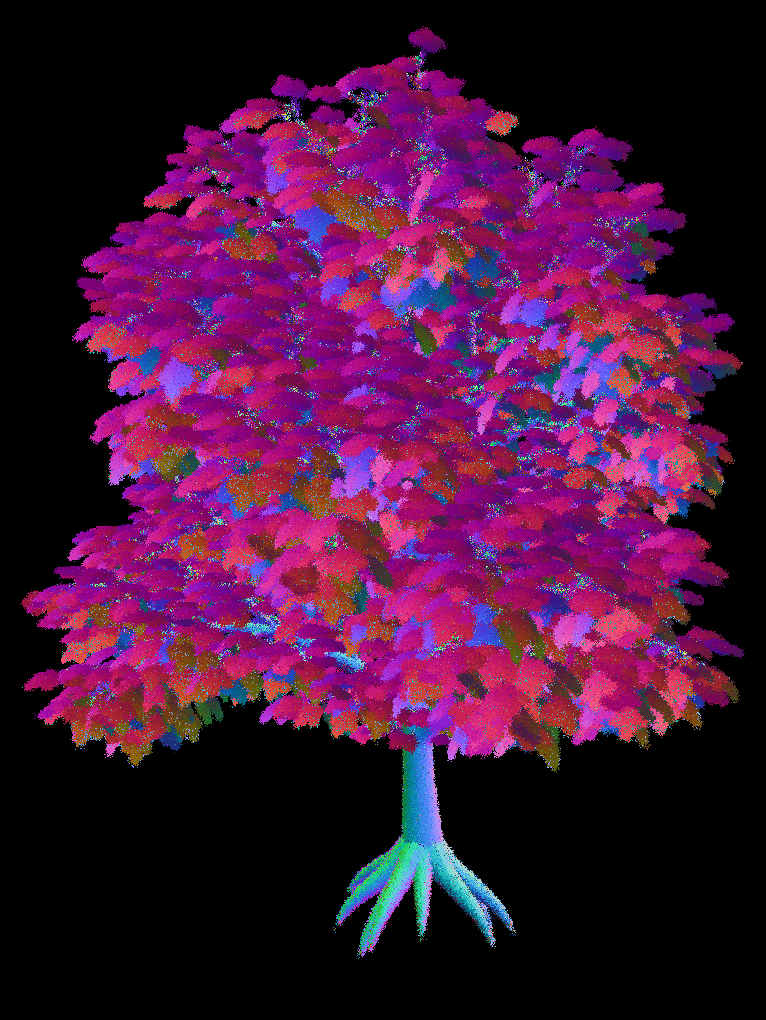
\includegraphics[width=1\linewidth]{img/normal_map_vndf_normal_aligned.png}
        \caption{}
        % \label{fig:bounding_size_1}
    \end{subfigure}
    \caption[Visualization of normals with meshes and volumes]{Visualization of the normals of the surface mesh (a), and of volumetric \acsp{lod} when the microflake normal is transformed with a coordinate frame around the direction $\omega_o$ (b) and when it is transformed with a coordinate frame around the filtered normal (c).
             Although being more blurry, transforming the microflake normal based on the filtered normal gives close results to the true normals.}
	\label{fig:tree_normal_maps}
\end{figure}
It is obvious, that transforming the microflake normal based on the outgoing direction $\omega_o$ gives different normals than the normals given by the mesh, while transforming it with a coordinate frame around the filtered normal gives normals that are distributed around the filtered normal.

Having sampled a reflection direction in the volume we move the origin of the new ray along this direction to the edge of the current voxel.
This is an idea by \citeauthor{vicini2021non} that prevents multiple scattering within a voxel \cite{vicini2021non}.
According to the authors multiple scattering can lead to paths passing through a voxel with a high density, which leads to an energy loss producing substantially darker looking volumes \cite{vicini2021non}.

\chapter{Results and Discussion}
\label{chap:results_and_discussion}
This chapter will present the results of the thesis and it discusses the limitations of our approach.
As mentioned before, we are interested in a sensible tradeoff between a performance improvement and a good image quality.
We therefore measure the render time of our \ac{lod} approach and the mesh ground truth.
The image quality is mainly determined by comparing the results visually to the ground truth, but we also provide the mean \FLIP \cite{flip} error to quantify the difference.
We choose this error because it gives a good approximation of the difference a human perceives when alternating between two images \cite{flip}.
For the sake of completeness, we also provide the mean \ac{ssim} and the \ac{psnr} in Appendix \ref{chap:psnr_and_ssim_errors}.
All images are rendered in our custom physically based path-tracer that we introduced in Section \ref{sec:rendering}.
We run the renderer on a system with an Intel Xeon E3-1230 v3 \ac{cpu}, 16 GB of RAM and a NVIDIA GeForce RTX 3060 \ac{gpu}.
We performed experiments on the forest scene with 9924 trees, which we present in Section \ref{sec:forest} and on single model instances, which we discuss in Section \ref{sec:experiments_on_single_model_instances}.
For the forest scene, we additionally analyze the memory usage, when using \acsp{lod}.

\section{Experiments on the Forest Scene}
\label{sec:forest}
As we explained, in Section \ref{sec:scene_generation} we choose our \acsp{lod} based on the heuristic that one voxel covers at most one pixel.
Figure \ref{fig:render_comparison} shows a rendering of a scene that was generated with this heuristic compared to a reference rendering that uses only meshes.
\begin{figure}[t]
    \centering
    \begin{subfigure}[b]{\linewidth}
        \resizebox{\textwidth}{!}{%
            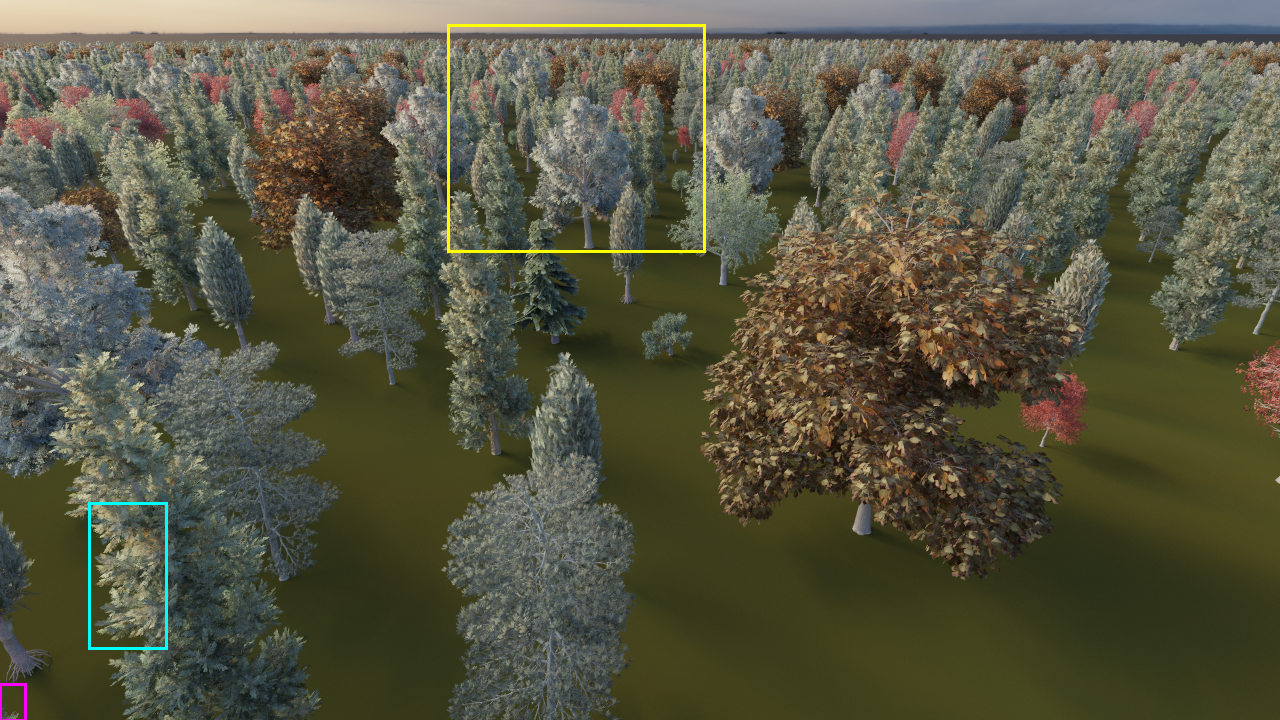
\includegraphics[height=4cm]{img/results/reference_with_boxes.png}%
            \quad
            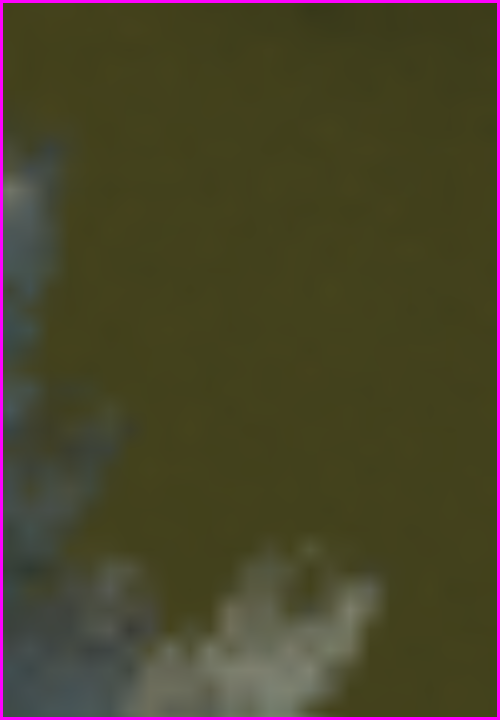
\includegraphics[height=4cm]{img/results/reference_snippet3.png}%
            \quad
            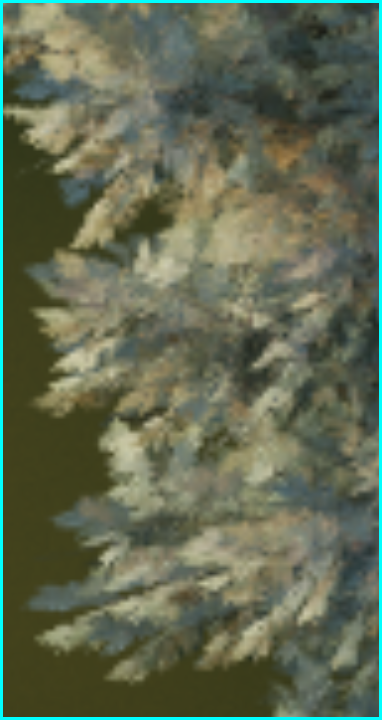
\includegraphics[height=4cm]{img/results/reference_snippet1.png}%
            \quad
            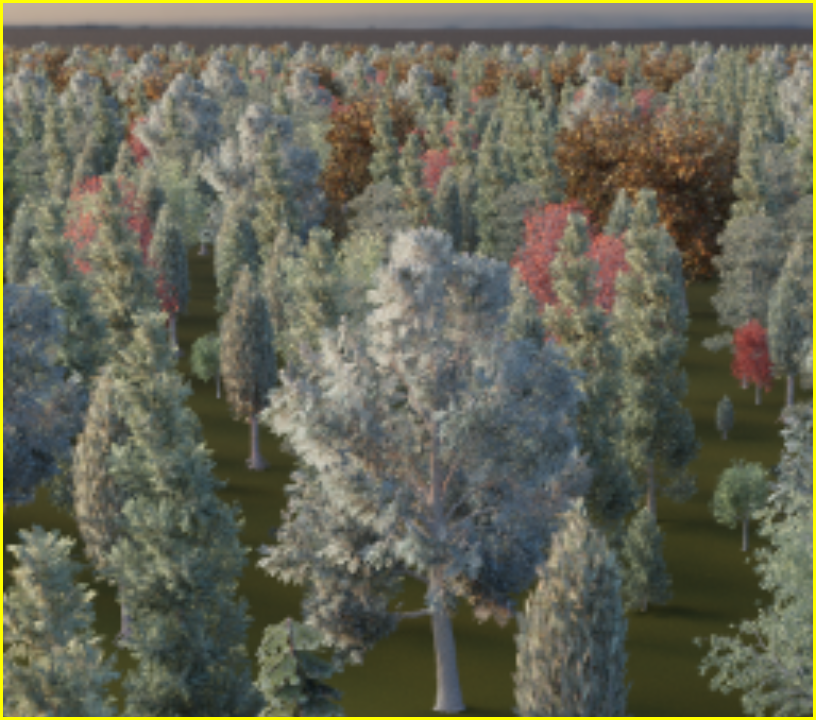
\includegraphics[height=4cm]{img/results/reference_snippet2.png}%
        }
        \caption{}
        \label{fig:render_comparison_mesh}
    \end{subfigure}
    \begin{subfigure}[b]{\linewidth}
        \resizebox{\textwidth}{!}{%
            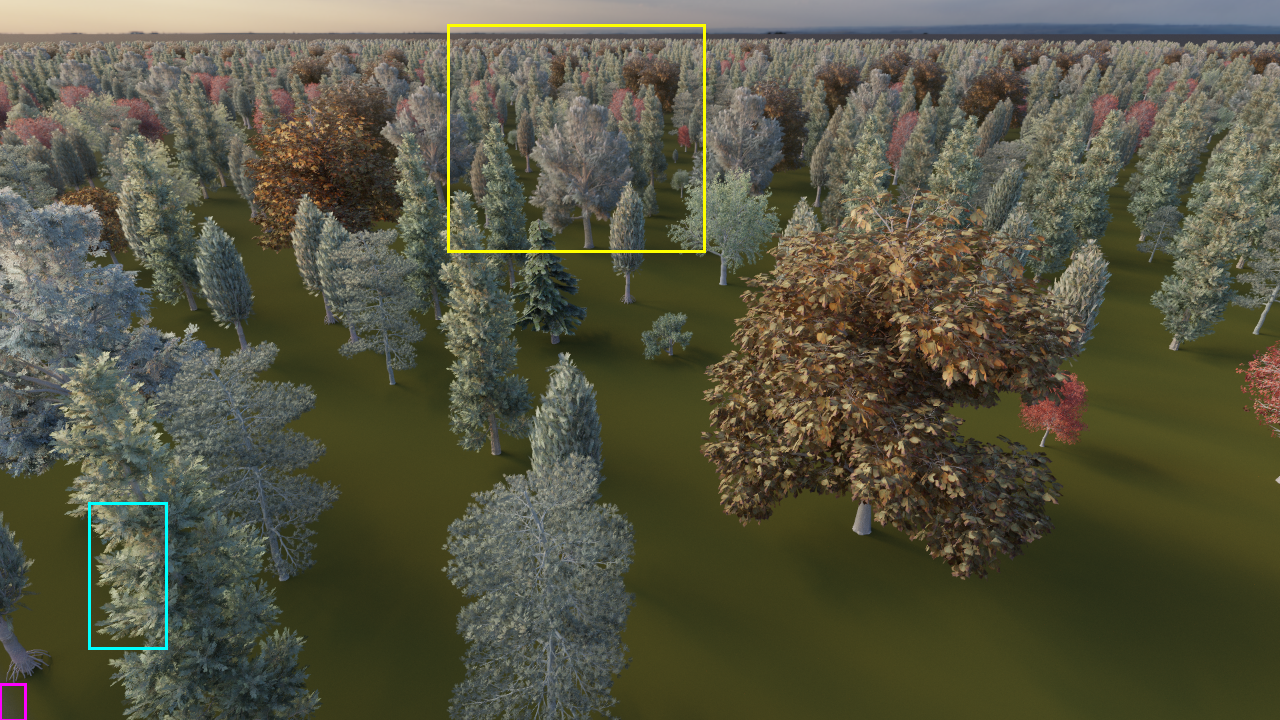
\includegraphics[height=4cm]{img/results/lod_1A_with_boxes.png}%
            \quad
            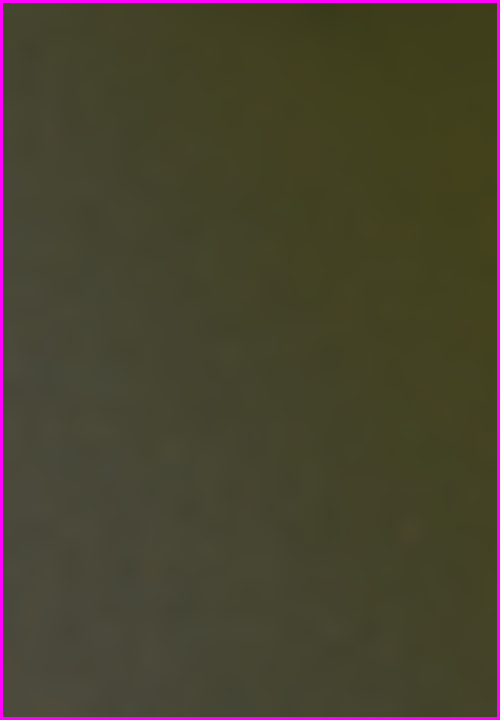
\includegraphics[height=4cm]{img/results/lod_1A_snippet3.png}%
            \quad
            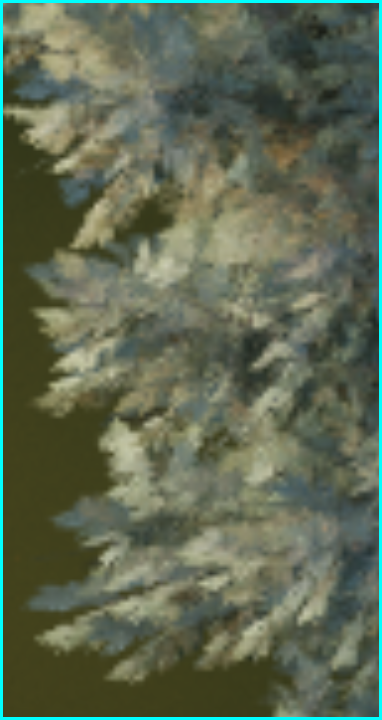
\includegraphics[height=4cm]{img/results/lod_1A_snippet1.png}%
            \quad
            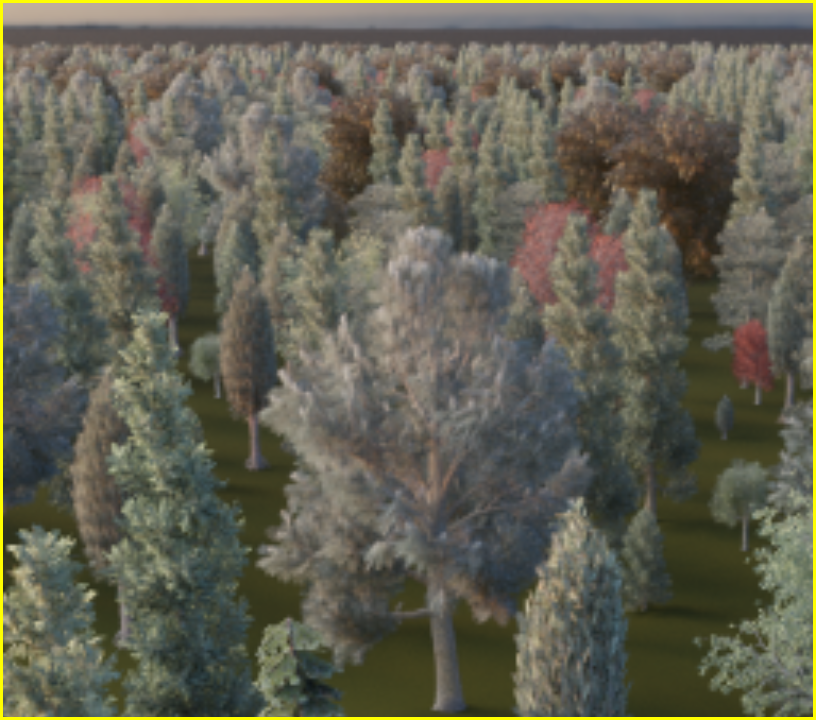
\includegraphics[height=4cm]{img/results/lod_1A_snippet2.png}%
        }
        \caption{}
        \label{fig:render_comparison_lod}
    \end{subfigure}
	\caption[Comparison between mesh and volume renderings of the forest]{(a) is the reference image rendered in $\SI{5463}{\s}$ with 1024 samples per pixel using only mesh representations, (b) uses \acsp{lod} if a voxel is smaller than a pixel and took $\SI{8723}{\s}$ to render with 1024 samples per pixel.}
	\label{fig:render_comparison}
\end{figure}
It can be observed that the structure of the volumetric trees cannot be distinguished from the mesh representations which speaks for our heuristic for \ac{lod} selection.
However, when we look at the yellow framed image segment, we see that the shading differs between both representations.
The volumetric trees generally look darker, which is especially pronounced on the side that faces the sun.
For our usage, the ray offsetting, that we introduced in Section \ref{sec:rendering}, showed only neglectable improvement of the shading.
In the magenta framed image segment, we can additionally see that a mesh is replaced by a volume, although it is clearly too close to the camera for the regular distance dependent \ac{lod} selection.
This is quite literally an edge case of our \ac{lod} selection procedure: We only check whether the vertices of the volumetric bounding box are within the view frustum, the edges connecting the vertices can still be visible in the frustum, thus also making the volume visible.
Unfortunately, we did not catch this shortcoming during development.
The differences in the cyan framed image segment are quite subtle: The tree in the reference rendering has a slight yellow tint that the \ac{lod} rendering lacks.
It is easier to see this error if we look at the \FLIP error map between the renderings from Figure \ref{fig:render_comparison} in Figure \ref{fig:error_map}.
\begin{figure}[t]
    \centering
    \resizebox{\textwidth}{!}{%
    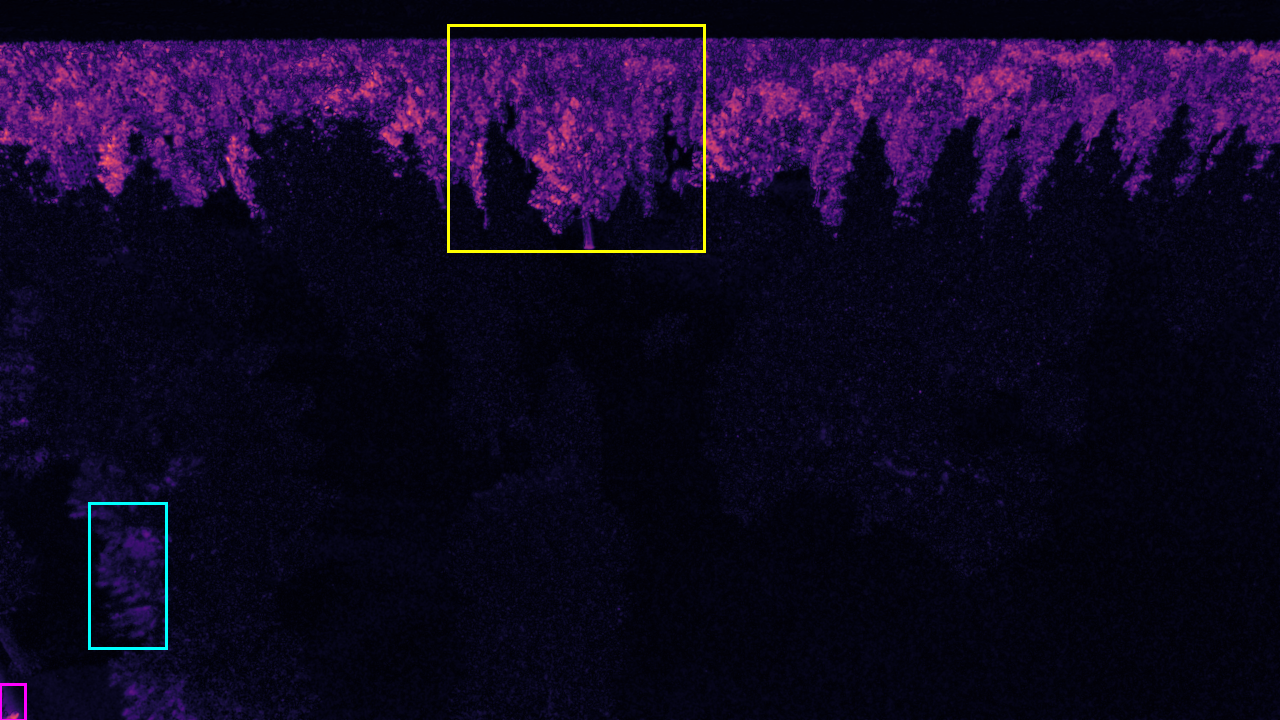
\includegraphics[height=4cm]{img/results/flip_error_1A_with_boxes.png}%
    \quad
    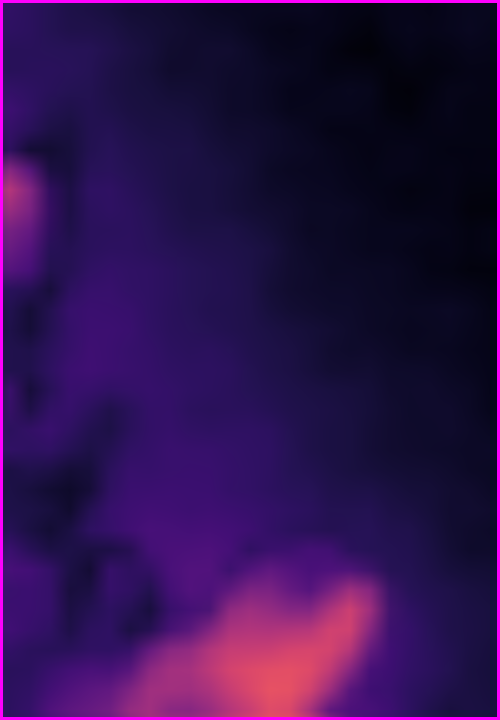
\includegraphics[height=4cm]{img/results/flip_error_1A_snippet3.png}%
    \quad
    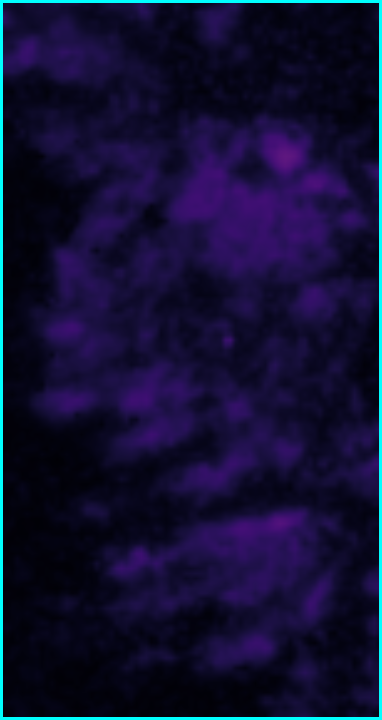
\includegraphics[height=4cm]{img/results/flip_error_1A_snippet1.png}%
    \quad
    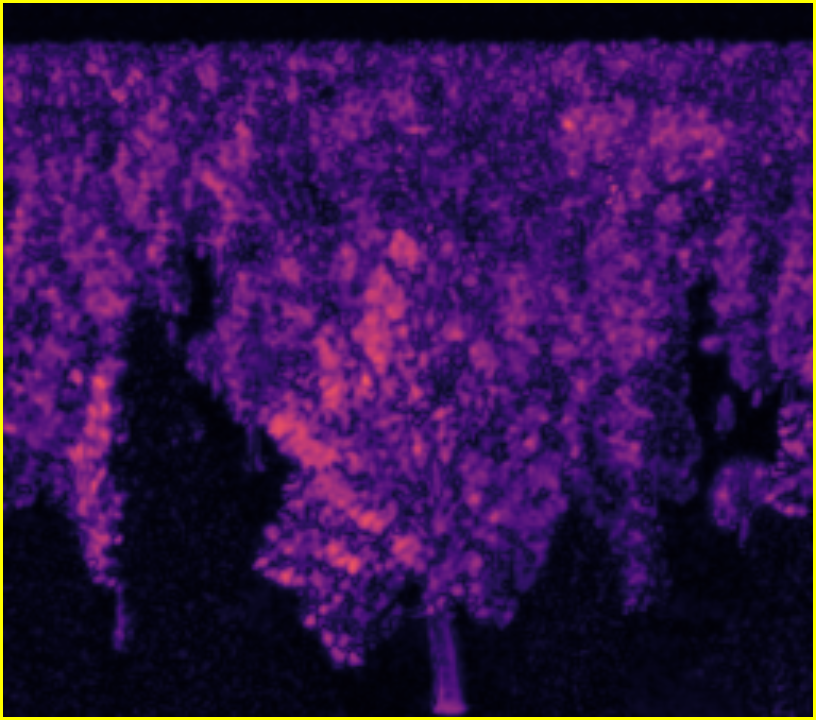
\includegraphics[height=4cm]{img/results/flip_error_1A_snippet2.png}%
    }
	\caption[\FLIP error map between reference and default \ac{lod} heuristic]{\FLIP error map between the reference rendering and the rendering using \acsp{lod} from Figure \ref{fig:render_comparison}. Dark regions indicate a low error, while bright regions indicate a high error. The mean \FLIP error is 0.073.}
	\label{fig:error_map}
\end{figure}
The tree in the cyan framed image segment visibly has an increased error compared to the surrounding trees.
This error is the result of indirect illumination: In the reference rendering there are mesh models outside the view frustum which reflect light on models in the view frustum.
These meshes outside the view frustum are replaced by volumes in the \ac{lod} rendering, which reflect less light.
The error map also makes the switch from mesh to volume rendering clearly visible, since the error suddenly increases.
As we observed in the renderings, the error is particularly high on the side that faces the sun.

In order to find the reason for the large shading difference on the sun-facing side, we split up the \acsp{brdf} and phase functions into the specular and diffuse component.
Intuitively we expect that these differences are specular highlights on the surfaces that are not rendered in the volumes.
However, looking at individual renderings of the diffuse and specular components in Figure \ref{fig:diffuse_specular_breakdown}, we find that these bright regions are in fact a result of the diffuse \ac{brdf}.
\begin{figure}[t]
    \centering
    \begin{subfigure}[b]{0.49\linewidth}
        \centering
        \includegraphics[width=1\linewidth]{img/results/diffuse_only_mesh.jpg}
        \caption{}
        % \label{fig:render_comparison_mesh}
    \end{subfigure}
    \begin{subfigure}[b]{0.49\linewidth}
        \centering
        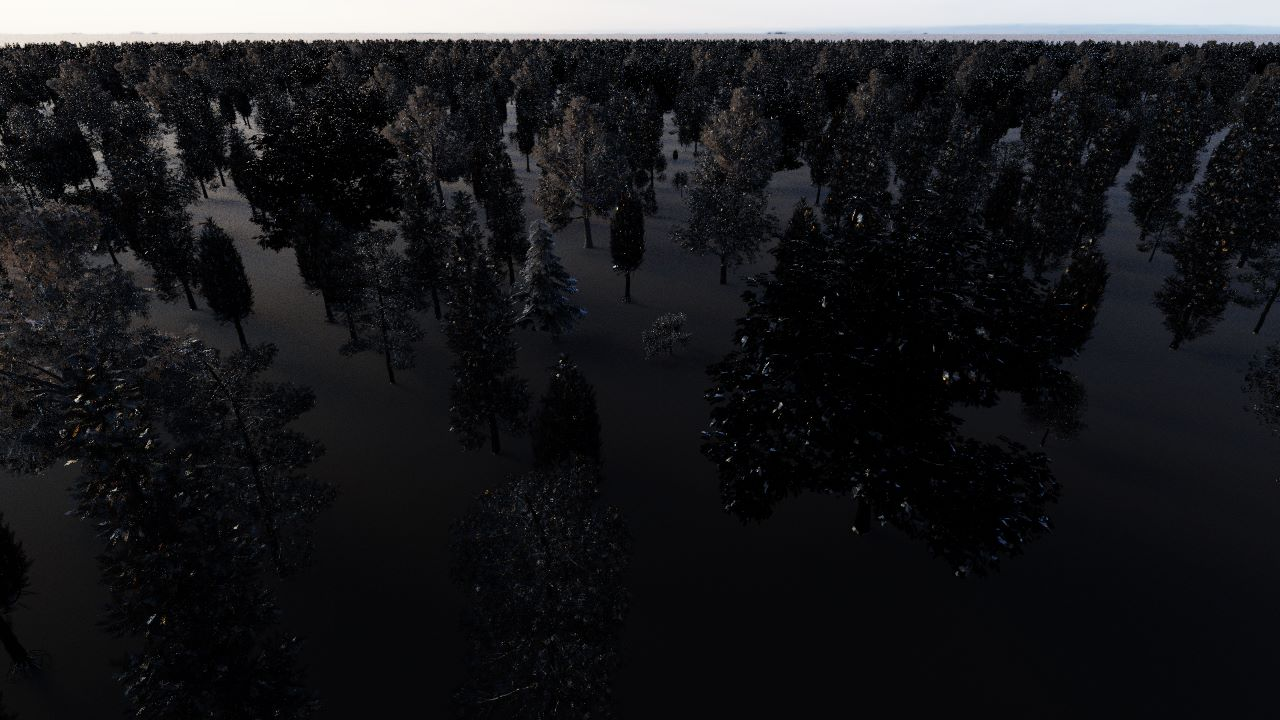
\includegraphics[width=1\linewidth]{img/results/specular_only_mesh.jpg}
        \caption{}
        % \label{fig:render_comparison_lod}
    \end{subfigure}
    \begin{subfigure}[b]{0.49\linewidth}
        \centering
        \includegraphics[width=1\linewidth]{img/results/diffuse_only_lod_1A.jpg}
        \caption{}
        % \label{fig:render_comparison_mesh}
    \end{subfigure}
    \begin{subfigure}[b]{0.49\linewidth}
        \centering
        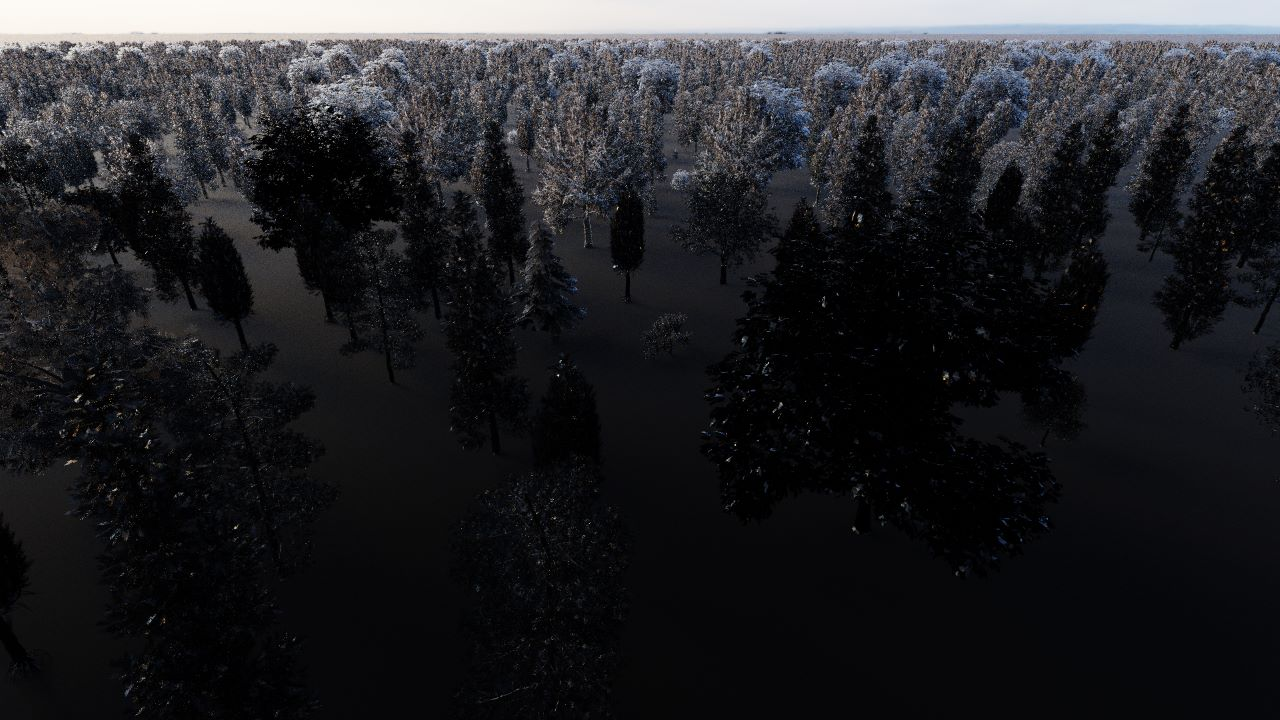
\includegraphics[width=1\linewidth]{img/results/specular_only_lod_1A.jpg}
        \caption{}
        % \label{fig:render_comparison_lod}
    \end{subfigure}
    % \caption[Comparison between mesh and volume renderings of the forest]{Renderings of the forest using meshes only (a) and using \acsp{lod} if a voxel is smaller than a pixel (b).}
    \caption[Diffuse and specular components rendered separately]{(a) and (b) respectively show the diffuse and specular components of the reference image, (c) and (d) respectively show the diffuse and specular components when using \acsp{lod} where a voxel covers at most one pixel. The images are rendered with 32 samples per pixel.}
	\label{fig:diffuse_specular_breakdown}
\end{figure}
In the volumes, the diffuse phase function gives way more uniform looking trees without these bright regions on the sun-facing side.
The specular component gives discrete specular highlights on the surfaces while the specular phase function leads to reflections across the whole medium.
So our approach fails in preserving the visual appearance of the meshes.
We identify two reasons for this limitation: First, the \ac{sggx} phase function is defined on the whole unit sphere (recall Figure \ref{fig:sggx_ndf}), which means that half of the rays are reflected into the medium where they are attenuated, while for surfaces all rays are reflected away from the surface.
Second, it is likely that this error occurred due to the usage of an isotropic microflake projected area, which directly influences our density values.
As we showed in Section \ref{sec:mesh_filtering} the optimization of the density depends on this projected area and by choosing a constant value we ignore for example how the roughness of a material influences the density, which would normally be reflected in the matrix $S$. % TODO: Maybe add example for effect of lowering roughness of leafs
Using an anisotropic projected area therefore can lead to a significantly different look.
The filtering procedure however, would become more complex.
Experiments in this direction are outside of the scope of this thesis.

% This affects our density values, since the density is also optimized based on the microflake projected area $sigma$.
%  which effectively leads to reflection directions that are uniformly scattered on the unit sphere.
% % Second, it is likely that this error is due to the usage of an isotropic extinction coefficient, which effectively leads to reflection directions that are uniformly scattered on the unit sphere.
% Therefore we could reduce the error by using an anisotropic extinction, which would lead to a more complex filtering procedure.

Apart from these visual problems, the render time for the \ac{lod} approach is another concern.
The duration with $\SI{8723}{\s}$ for 1024 samples per pixel (Figure \ref{fig:render_comparison_lod}) is currently slower than rendering only the meshes, which took $\SI{5463}{\s}$ for 1024 samples per pixel (Figure \ref{fig:render_comparison_mesh}).
As we just discussed, we recognize the \acsp{lod} mainly by their different color and not by their details or blurriness.
We therefore have some room left for tweaking the distance at which we switch to \ac{lod} rendering or we can use coarser \acsp{lod}.
Tweaking the distance translates to changing the number of pixels a voxel may cover.
As we wrote in Section \ref{sec:scene_generation}, our heuristic currently ensures that a voxel covers at most one pixel.
Now we relax this restriction and measure render times when a voxel covers 1, 4, 9 or 16 pixels.
Additionally, we test how changing the voxel size of the finest \ac{lod} affects the performance.
In the first experiment, the voxels in our finest \ac{lod} had a size of $\SI{0.1}{\m}$.
Now we choose a minimal voxel size of $\SI{0.1}{\m}$, $\SI{0.2}{\m}$, $\SI{0.4}{\m}$, $\SI{0.8}{\m}$, $\SI{1.6}{\m}$, $\SI{3.2}{\m}$ and $\SI{6.4}{\m}$.
In total this gives us 28 combinations.
% We visualize our measurements in Figure \ref{fig:render_durations} as a heat map.
In Figure \ref{fig:lod_grid} we visualize the durations as well as the \FLIP error for rendering the different configurations with 1024 samples per pixel.
\begin{figure}[t]
    \centering
    \begin{subfigure}[b]{0.49\linewidth}
        \centering
        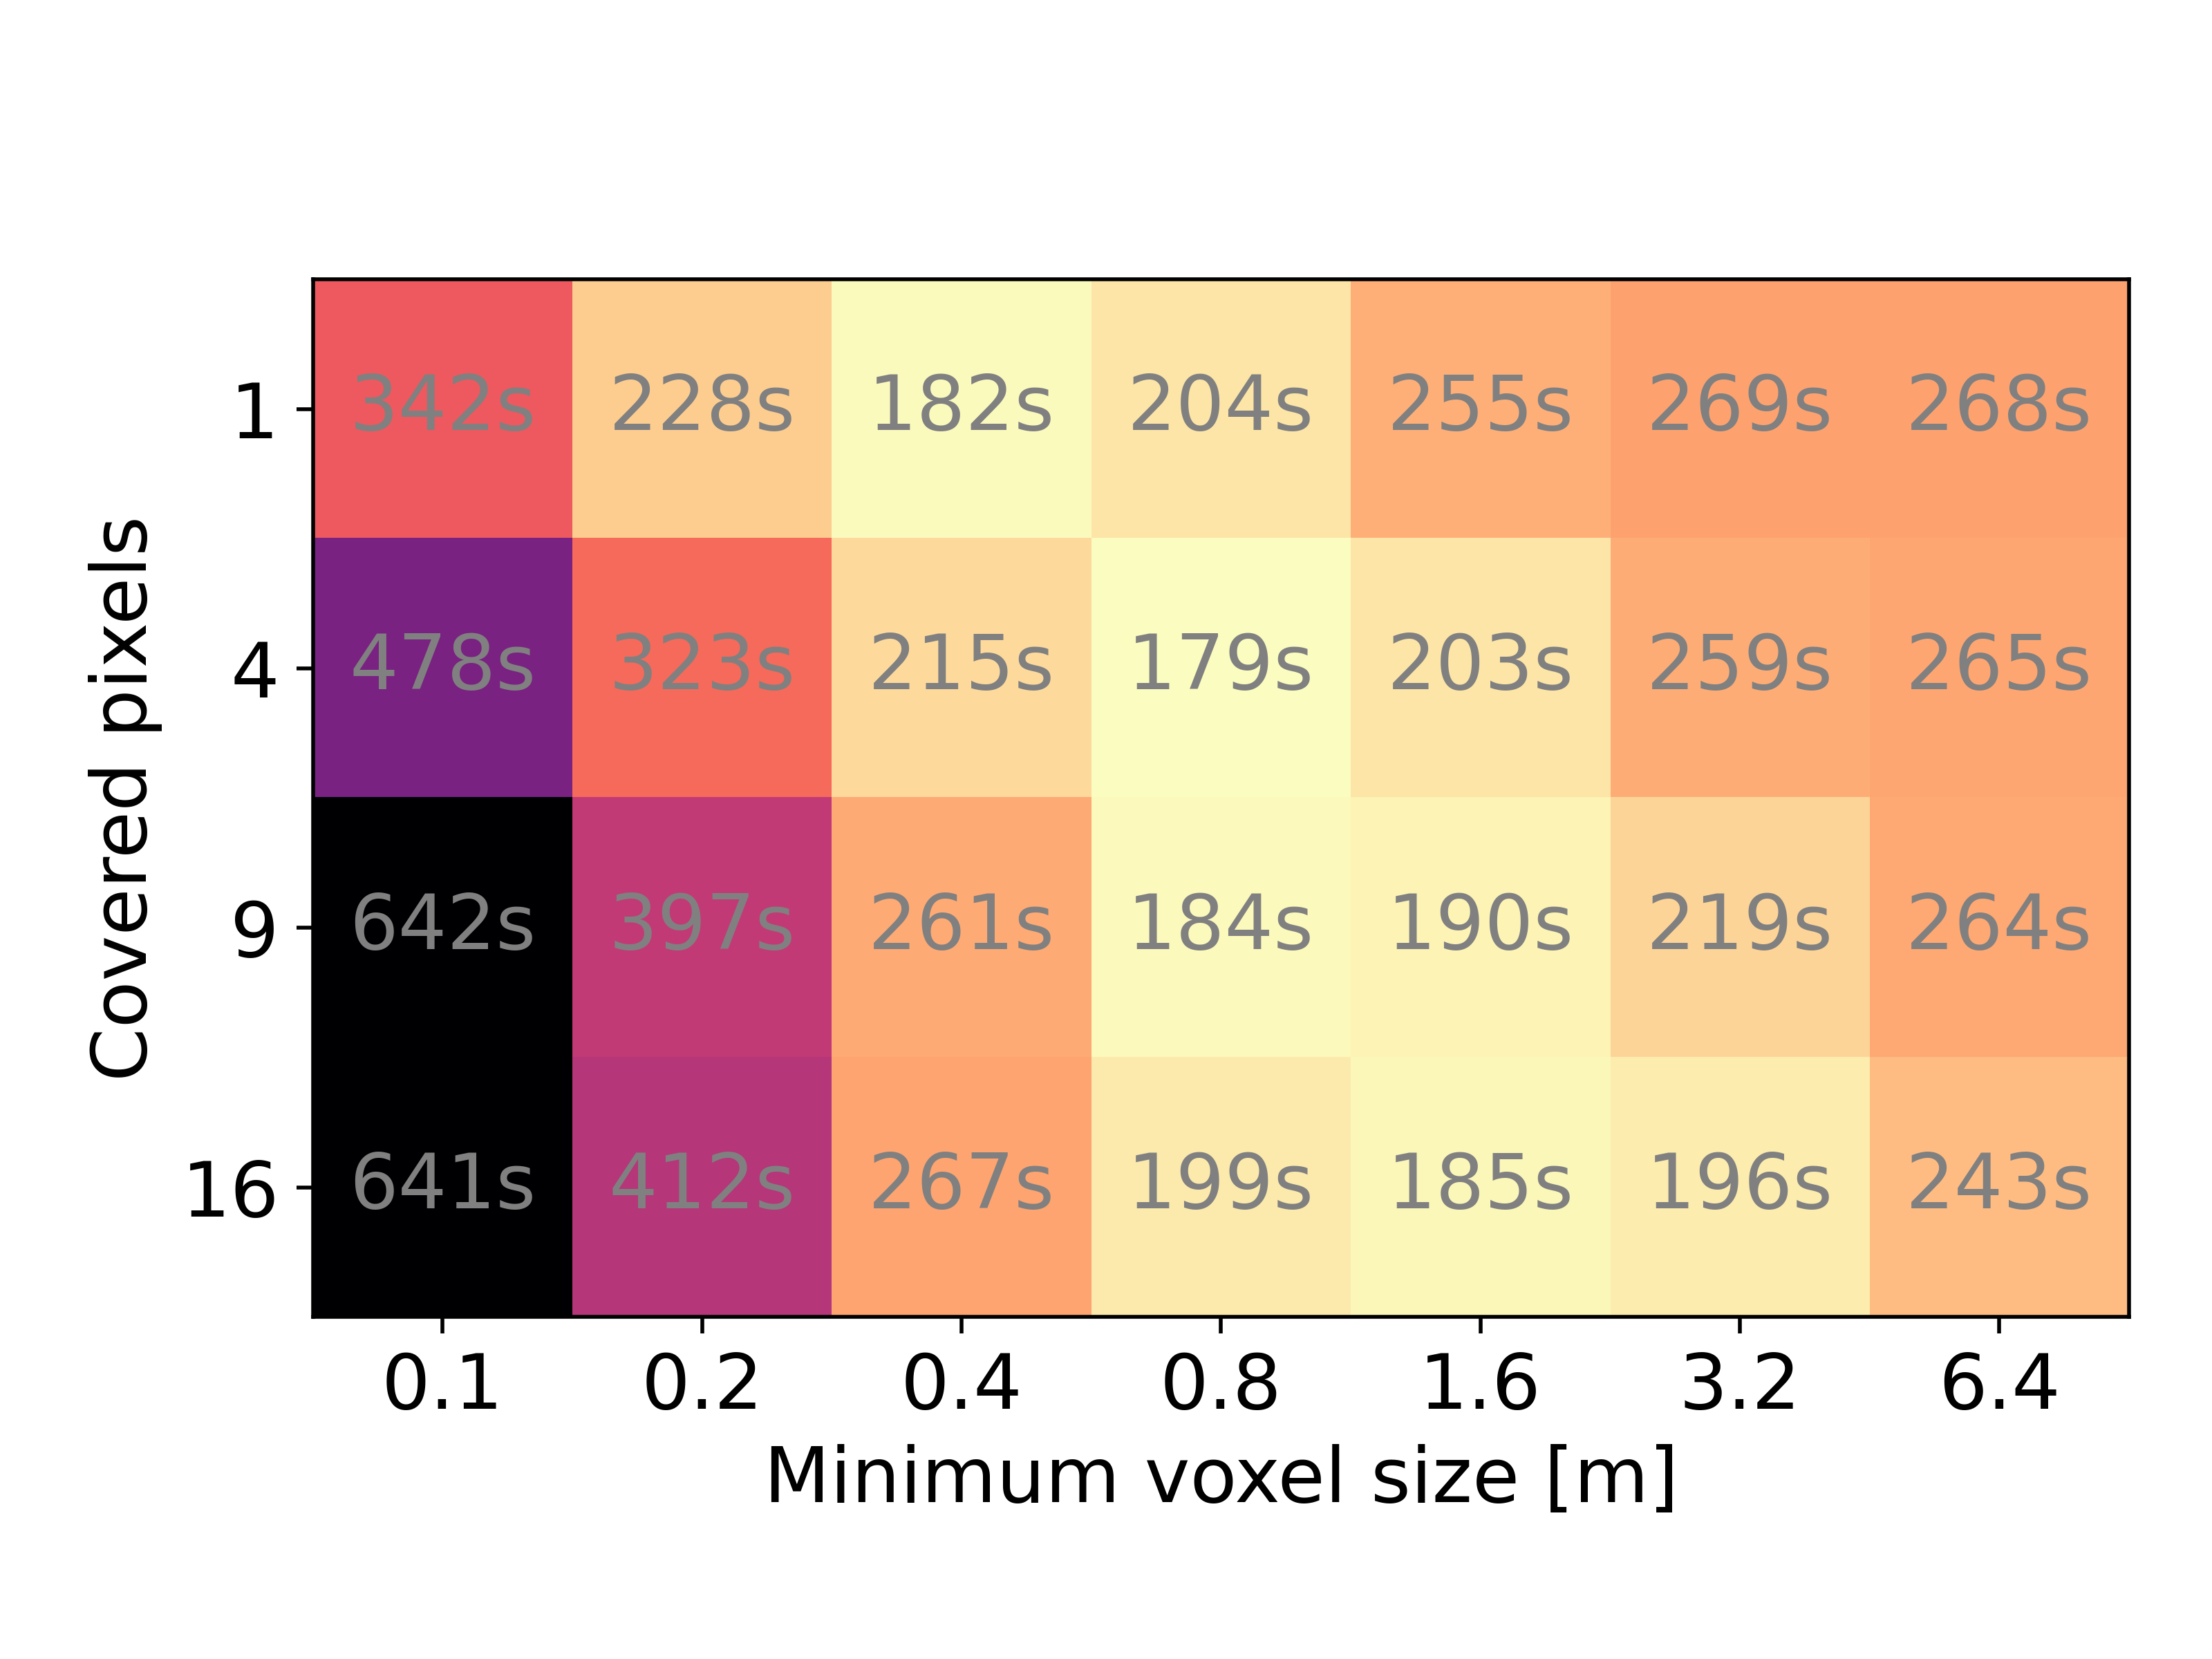
\includegraphics[width=1\linewidth]{img/results/render_durations.png}
        \caption{}
        \label{fig:lod_grid_durations}
    \end{subfigure}
    \begin{subfigure}[b]{0.49\linewidth}
        \centering
        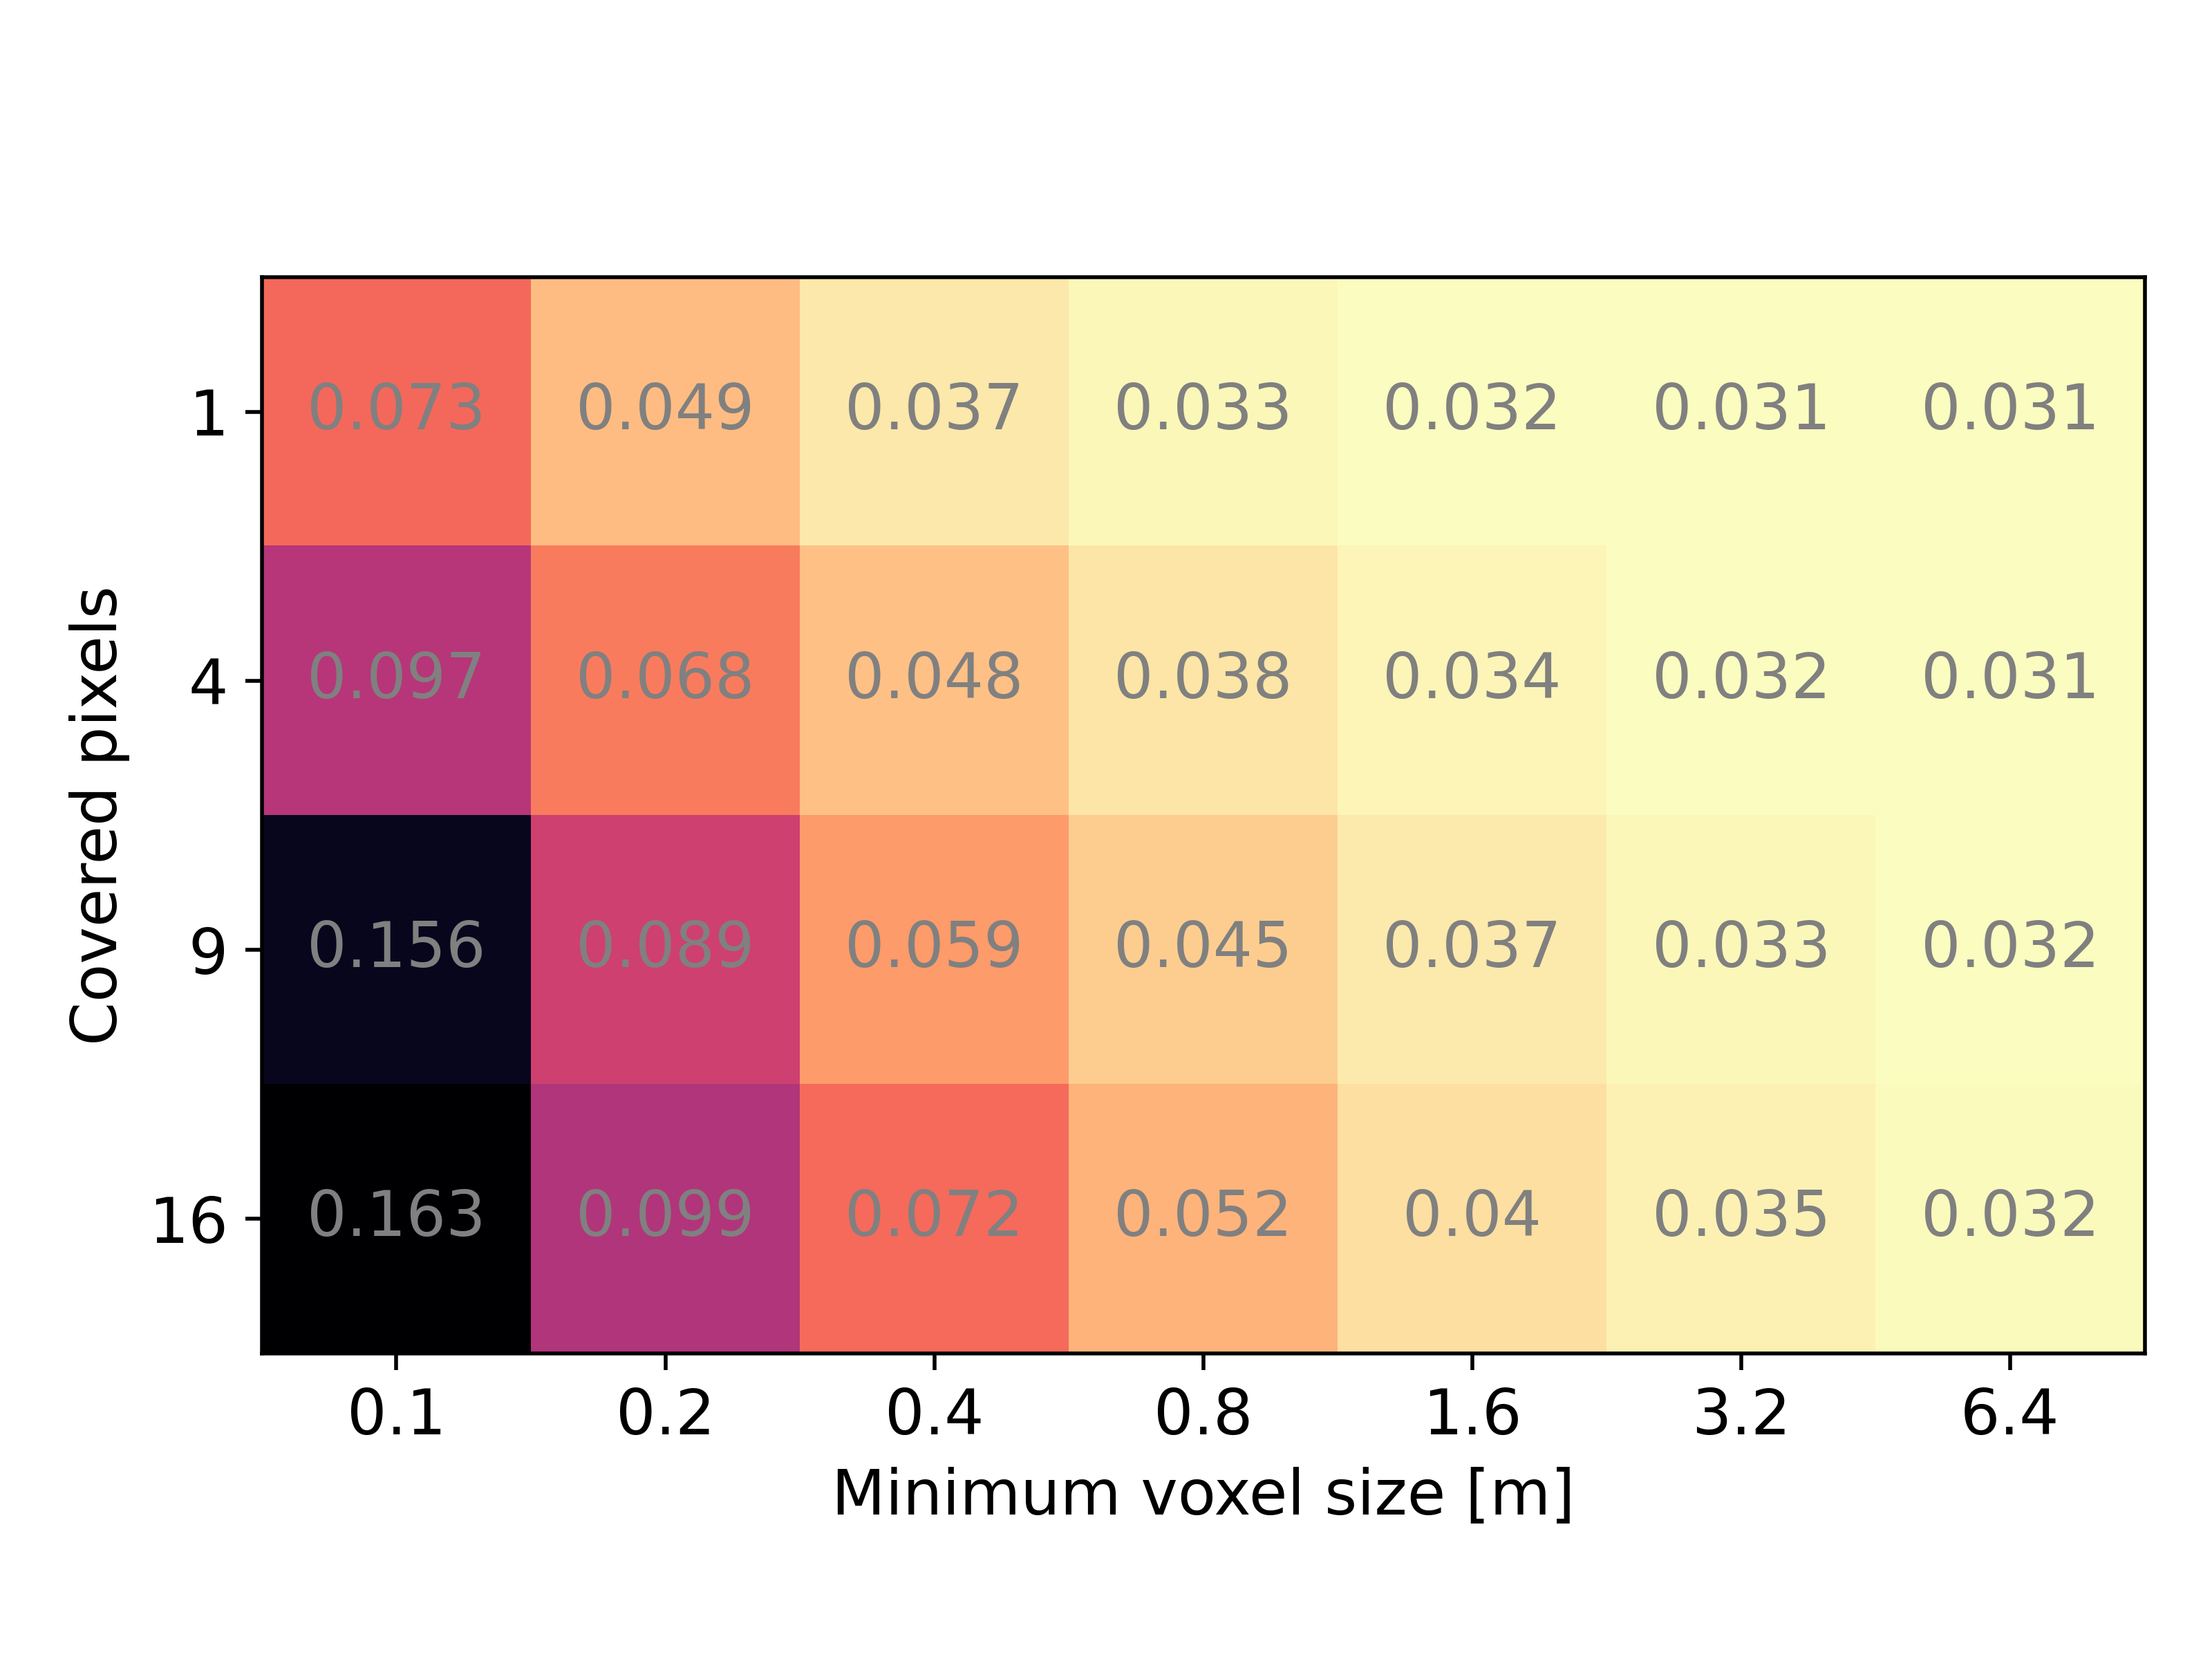
\includegraphics[width=1\linewidth]{img/results/flip_errors.png}
        \caption{}
        \label{fig:flip_errors}
    \end{subfigure}
	\caption[Heatmap of the \ac{lod} render durations and \FLIP errors]{Heatmap for render durations (a) and the mean \FLIP error (b) of different combinations of the minimum voxel size and the number of covered pixels. Bright regions indicate high values, dark regions indicate low values.}
	\label{fig:lod_grid}
\end{figure}
We can see that when we start \ac{lod} rendering with rougher \acsp{lod} we can reduce render times to a certain degree before they rise again.
The decline happens because rougher \acsp{lod} are less memory intensive then the fine \acsp{lod} and therefore easier to cache.
At the same time increasing the minimum voxel size for a fixed number of covered pixels pushes the boundary of the \ac{lod} switch away from the camera which increases the number of meshes to be rendered.
The meshes take longer to render than the rough \acsp{lod}, therefore the render time increases again.

We get another view on the different combinations between the number of covered pixels and the minimum voxel size if we visualize the bounding boxes, like we previously did in Figure \ref{fig:visualize_lods}.
Now we not only show a rendering from above the scene but also from the main camera perspective.
Figure \ref{fig:visualize_lods_different_configurations_covered_pixels_fixed} visualizes the previously described effect, that the distance at which \acsp{lod} are rendered increases, when the minimum voxel size is increased.
\begin{figure}[t]
    \begin{subfigure}[b]{\linewidth}
        \begin{center}
            \setlength{\tabcolsep}{2pt}
            \begin{tabular}{ c c c c  }
                \adjustimage{width=0.24\textwidth,valign=m}{img/results/visualize_lods_1A_front.jpg} & \adjustimage{width=0.24\textwidth,valign=m}{img/results/visualize_lods_1B_front.jpg} & \adjustimage{width=0.24\textwidth,valign=m}{img/results/visualize_lods_1C_front.jpg} & \adjustimage{width=0.24\textwidth,valign=m}{img/results/visualize_lods_1D_front.jpg} \\
                \adjustimage{width=0.24\textwidth,valign=m}{img/results/visualize_lods_1A_top.jpg} & \adjustimage{width=0.24\textwidth,valign=m}{img/results/visualize_lods_1B_top.jpg} & \adjustimage{width=0.24\textwidth,valign=m}{img/results/visualize_lods_1C_top.jpg} & \adjustimage{width=0.24\textwidth,valign=m}{img/results/visualize_lods_1D_top.jpg} \\
                {\footnotesize Covered pixels = 1} & {\footnotesize Covered pixels = 4} & {\footnotesize Covered pixels = 9} & {\footnotesize Covered pixels = 16} \\
            \end{tabular}
        \end{center}
        \caption{}
        \label{fig:visualize_lods_different_configurations_min_voxel_size_fixed}
    \end{subfigure}
    \begin{subfigure}[b]{\linewidth}
        \begin{center}
            \setlength{\tabcolsep}{2pt}
            \begin{tabular}{ c c c c  }
                \adjustimage{width=0.24\textwidth,valign=m}{img/results/visualize_lods_1A_front.jpg} & \adjustimage{width=0.24\textwidth,valign=m}{img/results/visualize_lods_2A_front.jpg} & \adjustimage{width=0.24\textwidth,valign=m}{img/results/visualize_lods_3A_front.jpg} & \adjustimage{width=0.24\textwidth,valign=m}{img/results/visualize_lods_4A_front.jpg} \\
                \adjustimage{width=0.24\textwidth,valign=m}{img/results/visualize_lods_1A_top.jpg} & \adjustimage{width=0.24\textwidth,valign=m}{img/results/visualize_lods_2A_top.jpg} & \adjustimage{width=0.24\textwidth,valign=m}{img/results/visualize_lods_3A_top.jpg} & \adjustimage{width=0.24\textwidth,valign=m}{img/results/visualize_lods_4A_top.jpg} \\
                % Covered pixels = 1 & Covered pixels = 4 & Covered pixels = 9 & Covered pixels = 16 \\
                {\footnotesize Min. voxel size = $\SI{0.1}{\m}$} & {\footnotesize Min. voxel size = $\SI{0.2}{\m}$} & {\footnotesize Min. voxel size = $\SI{0.4}{\m}$} & {\footnotesize Min.\newline voxel size = $\SI{0.8}{\m}$}\\
            \end{tabular}
        \end{center}
        \caption{}
        \label{fig:visualize_lods_different_configurations_covered_pixels_fixed}
    \end{subfigure}
    \caption[Visualization of \acsp{lod} using different configurations]{Debug views of the volume bounding boxes for different configurations. In (a) the minimum voxel size is fixed at $\SI{0.1}{\m}$ and we vary the number of covered pixels, while in (b) the number of covered pixels is fixed at 1 and we vary the minimum voxel size. Blue is the finest \ac{lod} and red the coarsest \ac{lod}. }
    \label{fig:visualize_lods_different_configurations}
\end{figure}
For the case of a fixed number of covered pixels and a minimum voxel size of $\SI{0.8}{\m}$, it is also interesting to note that the distance based \acsp{lod} still cover almost half of the circular forest, although they are barely visible from the main camera's perspective.
Figure \ref{fig:visualize_lods_different_configurations_min_voxel_size_fixed} on the other hand, is analogous to the first column of Figure \ref{fig:lod_grid_durations}, as we also fixed the minimum voxel size at $\SI{0.1}{\m}$ and increase the number of covered pixels.
The figure intuitively explains the near doubling of the render time between 1 covered pixel and 16 covered pixels, since we start \ac{lod} rendering right in front of the camera for 16 covered pixels.


% We get another view on the increasing distances of \ac{lod} rendering when we look at the colored bounding boxes of the volumes again ...
Looking back at Figure \ref{fig:lod_grid}, the overall best result is achieved by dropping the three finest \acsp{lod} and let each voxel cover up to four pixels.
The scene then renders in $\SI{4549}{\s}$ which is a 17\% improvement over rendering only meshes.
Additionally, it has the positive side-effect that the shading problem is less noticeable, which is reflected in a drop in the mean \FLIP error from 0.073 to 0.038.
Figure \ref{fig:render_and_error_fastest} shows this rendering with the corresponding \FLIP error map.
\begin{figure}[t]
    \centering
    \begin{subfigure}[b]{\linewidth}
        \resizebox{\textwidth}{!}{%
            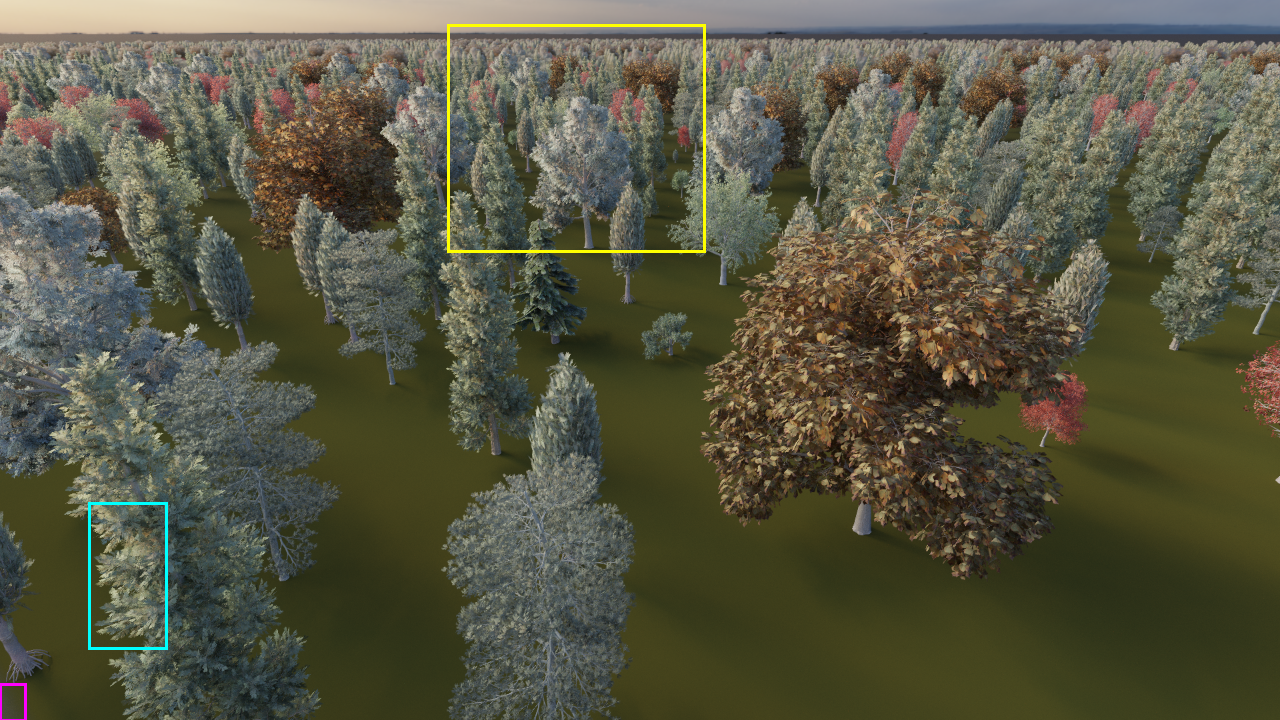
\includegraphics[height=4cm]{img/results/lod_4B_with_boxes.png}%
            \quad
            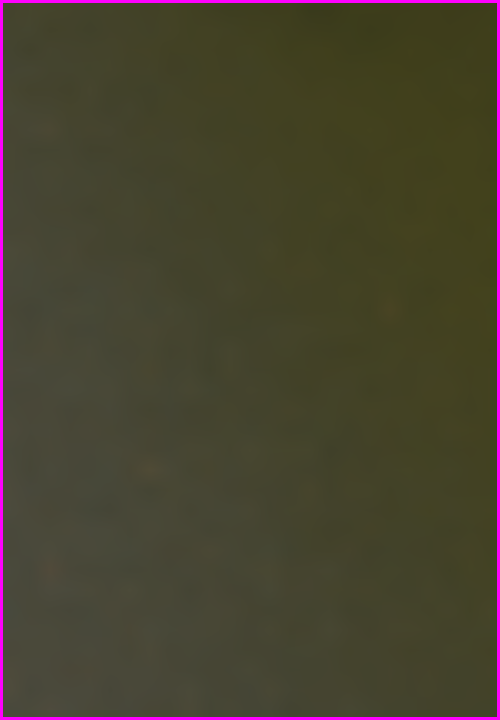
\includegraphics[height=4cm]{img/results/lod_4B_snippet3.png}%
            \quad
            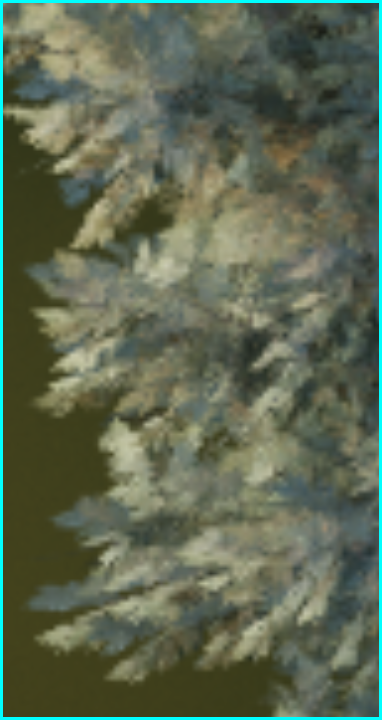
\includegraphics[height=4cm]{img/results/lod_4B_snippet1.png}%
            \quad
            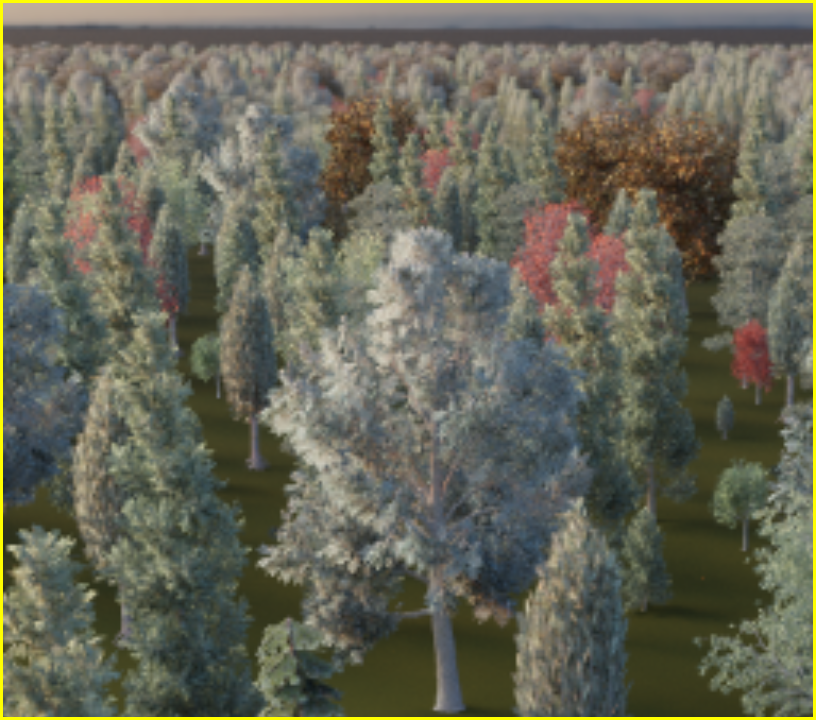
\includegraphics[height=4cm]{img/results/lod_4B_snippet2.png}%
        }
        \caption{}
    \end{subfigure}
    \begin{subfigure}[b]{\linewidth}
        \resizebox{\textwidth}{!}{%
            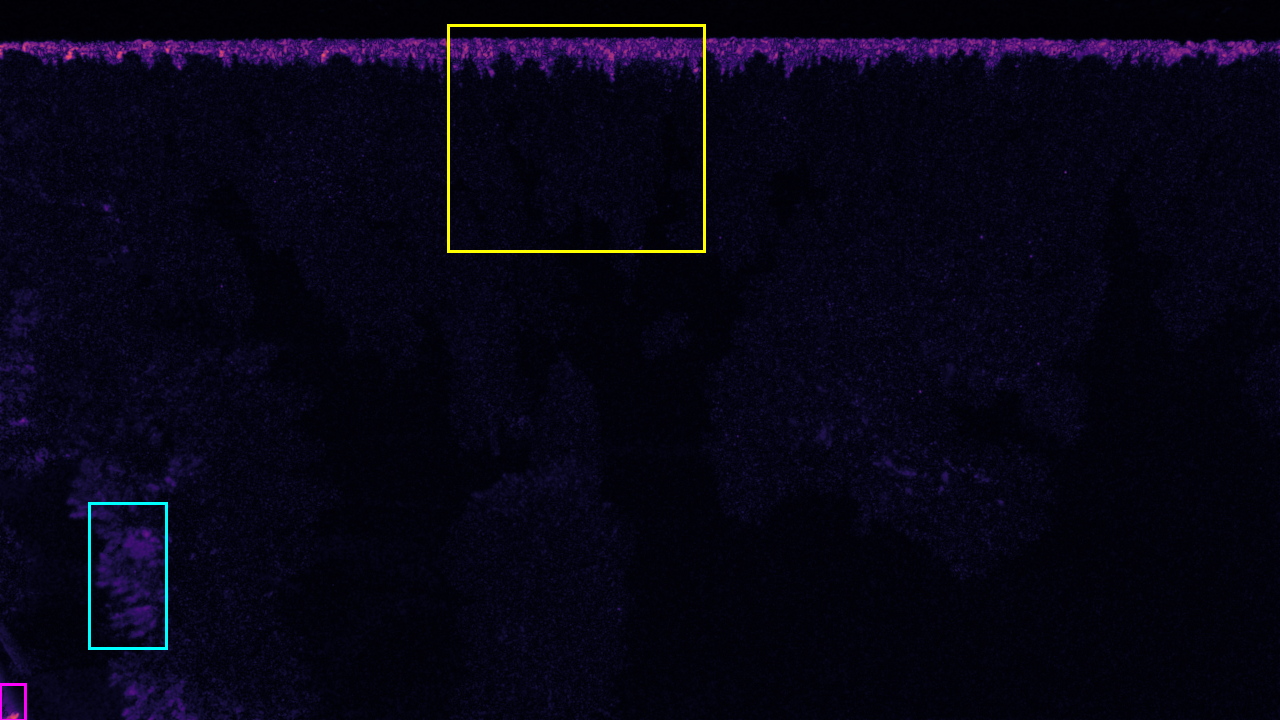
\includegraphics[height=4cm]{img/results/flip_error_4B_with_boxes.png}%
            \quad
            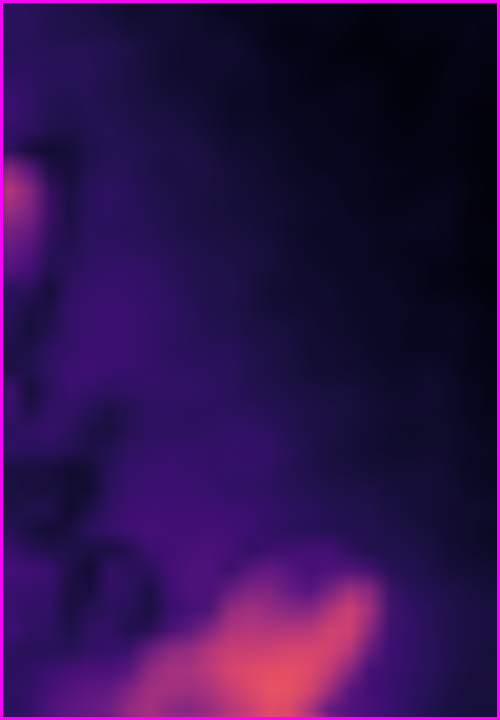
\includegraphics[height=4cm]{img/results/flip_error_4B_snippet3.png}%
            \quad
            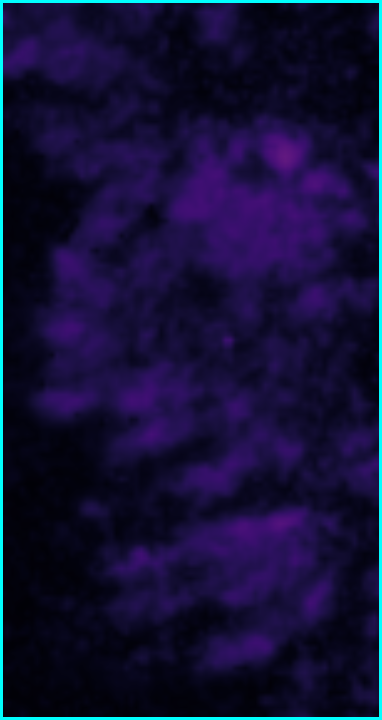
\includegraphics[height=4cm]{img/results/flip_error_4B_snippet1.png}%
            \quad
            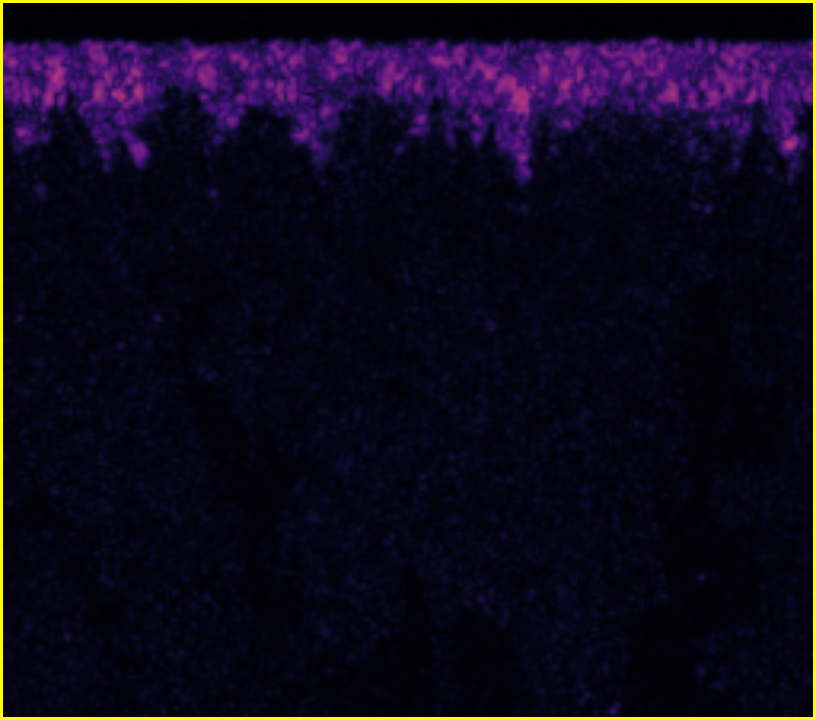
\includegraphics[height=4cm]{img/results/flip_error_4B_snippet2.png}%
        }
        \caption{}
    \end{subfigure}
    \caption[Rendering and \FLIP error map of the fastest combination]{(a) shows the fastest configuration, finished in $\SI{4548}{\s}$ for 1024 samples. The scene is generated with a minimum voxel size of $\SI{0.8}{\m}$ and up to four covered pixels per voxel. (b) shows the corresponding \FLIP error map against the ground truth. The mean \FLIP error is 0.038.}
    \label{fig:render_and_error_fastest}
\end{figure}
We can further decrease the mean \FLIP error down to 0.031, for example, by choosing a minimum voxel size of 6.4 meters and let each voxel cover one pixel, at the cost of a higher render time.

The last experiment we perform on the forest scene analyzes the memory consumption of the different configurations of the number of covered pixels and the minimum voxel size.
Since we use instancing of the geometry, texture and volume grids, the memory footprint between all configurations is roughly the same.
But we can analyze how much memory is used if we would not use instancing.
This gives us an idea, how our approach performs regarding memory consumption, if we had many distinct models in the scene, which is typical for feature films.
This analysis could also be interesting if the scene's assets need to be streamed over a network and the load on the network has to be minimized.
Due to system limitations, we cannot render such scenes anymore, but it is enough to know the memory usage of each model's \ac{lod} and the distibution of the model's \acsp{lod} in a scene to obtain the total memory consumption.
Without instancing, the reference scene would consume $\SI{830}{GB}$ of memory.
As Figure \ref{fig:memory_usage} visualizes in the familiar heatmap, we can reduce this footprint, by choosing any of the different \ac{lod} configurations.
\begin{figure}[t]
    \centering
    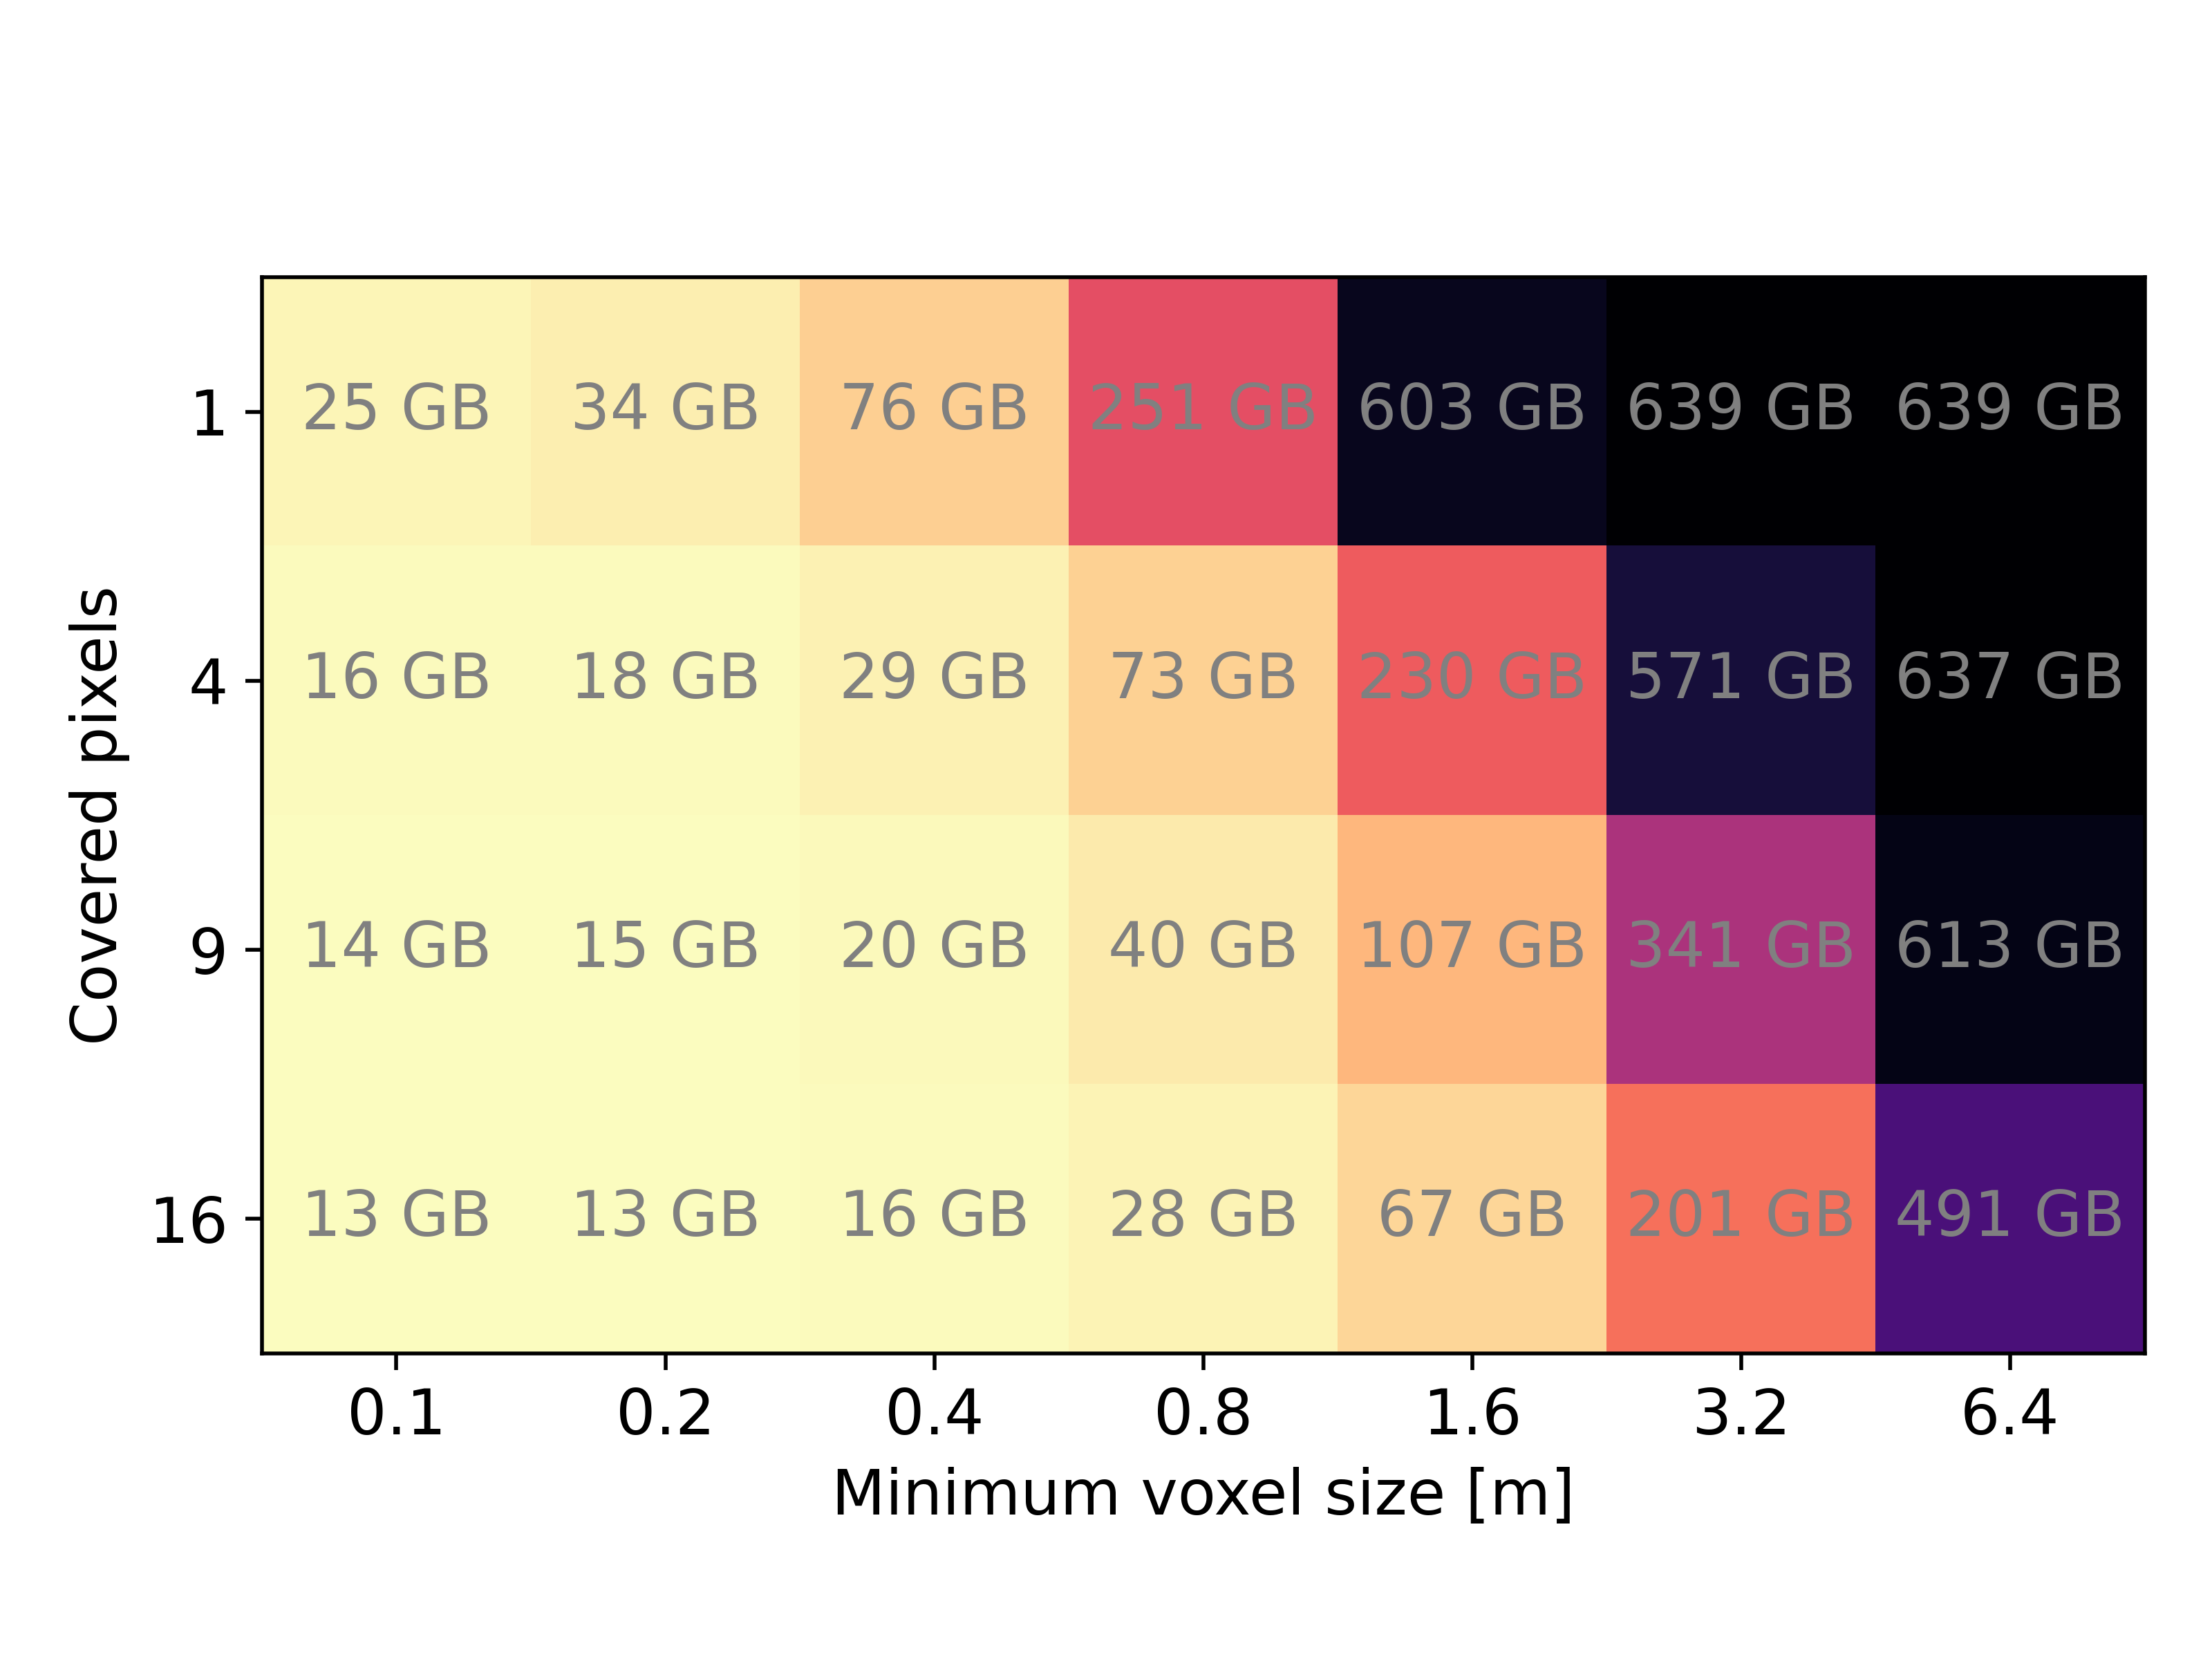
\includegraphics[width=0.49\linewidth]{img/results/memory_usage.png}
    \caption[Visualization of the memory consumption of different scene configurations]{Heatmap of the memory consumptions of different scene configurations when using no instancing. Bright regions indicate low memory usage, dark regions indicate high memory usage.}
    \label{fig:memory_usage}
\end{figure}
It is obvious, that with increasing minimum voxel sizes, the memory usage increases as well.
However, increasing the number of pixels that a voxel may cover, reduces the memory consumption.
Comparing Figure \ref{fig:memory_usage} and Figure \ref{fig:flip_errors}, we see that a high memory consumption correlates with a low \FLIP error, while a low memory footprint correlates with a high \FLIP error.
The memory consumption therefore behaves inverse to the \FLIP error.
Interestingly, the configuration with the lowest render time from Figure \ref{fig:lod_grid_durations}, does not have the smallest memory footprint.
We can therefore conclude, that the memory consumption is not the only variable that plays into the render time of a scene.

\section{Experiments on Single Model Instances}
\label{sec:experiments_on_single_model_instances}
Now that we have a good idea of the performance and quality implications of our approach, we perform further tests on single instances of some tree models.
This gives us finer control over which \ac{lod} should be rendered at which distance.
We use the models \textit{Celtis australis adult} (Figure \ref{fig:EU06a}) and \textit{Acer rubrum adult} (Figure \ref{fig:EA01a}) for our tests. % TODO: Maybe use PR04a instead
\begin{figure}[t]
    \centering
    \begin{subfigure}[b]{0.49\linewidth}
        \centering
        \includegraphics[width=1\linewidth]{img/results/EU06a.png}
        \caption{}
        \label{fig:EU06a}
    \end{subfigure}
    \begin{subfigure}[b]{0.49\linewidth}
        \centering
        \includegraphics[width=1\linewidth]{img/results/EA01a.png}
        \caption{}
        \label{fig:EA01a}
    \end{subfigure}
	\caption[Models for single instance experiments]{We use the model \textit{Celtis australis adult} (a) and \textit{Acer rubrum adult} (b) for our single instance experiments. Both images show the mesh representations.}
	\label{fig:single_model_instances}
\end{figure}

As a first experiment, we render a single instance of all mesh and volume representations at different distances.
We can see the render times of this experiment plotted in Figure \ref{fig:render_time_comparisons}.
\begin{figure}[t]
    \centering
    \begin{subfigure}[b]{0.49\linewidth}
        \centering
        \includegraphics[width=1\linewidth]{img/results/render_durations_EU06a.png}
        \caption{}
    \end{subfigure}
    \begin{subfigure}[b]{0.49\linewidth}
        \centering
        \includegraphics[width=1\linewidth]{img/results/render_durations_EA01a.png}
        \caption{}
    \end{subfigure}
	\caption[Plots of the render times depending on the distance from the camera]{These plots show the render times depending on the distance from the camera for single instances of the model \textit{Celtis australis adult} (a) and for \textit{Acer rubrum adult} (b). Meshes render faster than all \acsp{lod} until a certain distance.}
	\label{fig:render_time_comparisons}
\end{figure}
Interestingly, the meshes first render faster than all \acsp{lod}.
With increasing distance the render times of the volumetric representations then decrease rapidly and eventually fall below the render time of the mesh representation.
For the model \textit{Celtis australis adult} this is the case after $\SI{800}{\m}$ and for the model \textit{Acer rubrum adult} a \ac{lod} renders faster after $\SI{700}{\m}$.
Surprisingly, the render times for the mesh representations only decline in the beginning, but after a certain distance they rise steadily.
An explanation for this could be that at a certain distance the random sampling of a pixel produces large jumps across the bounding volume hierarchy, which leads to many cache misses.


As a second experiment we want to fix the distance between the camera and the model and measure how the image quality in terms of the \FLIP error and render times change when we choose different \acsp{lod}.
Since the model covers only a small area of the image, we crop the image before we compute the \FLIP error.
\begin{figure}[t]
    \centering
    \begin{subfigure}[b]{0.49\linewidth}
        \centering
        \includegraphics[width=1\linewidth]{img/results/performance_quality_EU06a.png}
        \caption{}
    \end{subfigure}
    \begin{subfigure}[b]{0.49\linewidth}
        \centering
        \includegraphics[width=1\linewidth]{img/results/performance_quality_EA01a.png}
        \caption{}
    \end{subfigure}
	\caption[Plots of \FLIP error and render times for different \acsp{lod}]{These plots show the render times and mean \FLIP errors for different \acsp{lod}. Again, (a) shows the results for a single instance of the \textit{Celtis australis adult} model and (b) shows the results for \textit{Acer rubrum adult}. The \FLIP error is computed on a relevant image segment.}
	\label{fig:performance_quality}
\end{figure}
We observe in Figure \ref{fig:performance_quality} that the render times fall in an exponential fashion, while the \FLIP errors show logarithmic growth.
Note however, that the voxel sizes of our \acsp{lod} increase exponentially by construction, which we have to consider in our interpretation.
We could alternatively draw the plots over the linear \ac{lod} level instead of the exponentially growing voxel size.
Regardless of the choice of the abscissa, the plots visualize the tradeoff well that we have to make: We can either improve the performance by choosing rougher \acsp{lod} which leads to a high image error.
Or we aim for a high image quality by selecting a detailed \ac{lod}, which leads to longer render times.
Another observation that we made during the single instance rendering is that the approach by \citeauthor{vicini2021non} of offsetting the scattered ray to the voxel border impairs the quality of the representation.
\begin{figure}[t]
    \centering
    \begin{subfigure}[b]{0.49\linewidth}
        \centering
        \includegraphics[width=1\linewidth]{img/results/EU06a_6.4.png}
        \caption{}
    \end{subfigure}
    \begin{subfigure}[b]{0.49\linewidth}
        \centering
        \includegraphics[width=1\linewidth]{img/results/EA01a_6.4.png}
        \caption{}
    \end{subfigure}
	\caption[Renderings of volumes with a voxel size of $\SI{6.4}{\m}$]{Renderings of the \acsp{lod} with a voxel size of $\SI{6.4}{\m}$ of the model \textit{Celtis australis adult} (a) and \textit{Acer rubrum adult} (b). The voxel borders are visible due to the ray offsetting.}
	\label{fig:rough_lods}
\end{figure}
This is especially pronounced when rough \acsp{lod} are viewed from a close distance.
Figure \ref{fig:rough_lods} shows the effect of the ray offsetting on the \acsp{lod} with a voxel size of $\SI{6.4}{\m}$.
The voxel borders are clearly visible in these renderings, since the transmission of a ray is not updated by the offset.
For close-up renderings of fine \acsp{lod} this artifact is less visible and in landscape scenes, like the forest scene from Section \label{sec:forest_experiments}, we were not able to perceive it.









\chapter{Future Work}
\label{chap:future_work}
As we discovered, the abilities of our approach to preserve the look of the surface mesh is not satisfactory.
The next step to improve on this would be to include anisotropic extinction, which would require a rewrite of the filtering procedure and the distance sampling and transmittance estimation.
The existing volumes would not be compatible with this new approach and had to be re-generated as well.

To further enhance the quality of the renderings, it would be interesting how our volumetric \ac{lod} approach performs with spectral rendering.
This would improve physical accuracy since the scattering in media is actually wavelength dependent \cite{novak_overview} but it requires a rewrite of the renderer.
Since this increases the dimension of the rendering equation it leads to an increase in the render duration and is currently only feasible for offline rendering.
A performance improvement should still be the result.

Another interesting area of research would be to further improve the performance of our approach and possibly switch the \acsp{lod} on the fly.
This would allow a camera movement without making the \acsp{lod} misalign the current view frustum.
The scene generator would have to be written in C++ for that and optimization of the program itself have to be made.
A large improvement can be expected by caching the free positions in the forest area, since we initialize the random number generator with the same seed anyway.
However this is limited to our forest scene.
A more portable optimization would be to approximate the pixels a bounding box covers by a rectangle instead of the convex hull that we currently use.
Also using brick grid for storing all voxel attributes like color values or the \ac{sggx} matrix $S$ might be worth investigating regarding the performance implications.

Having the knowledge that rough \acsp{lod} do not necessarily render faster than meshes, a further optimization would be to not simply set models outside of the view frustum to the roughest \ac{lod}.
Instead it might be beneficial to also incorporate the distance to the camera for these and use the mesh representations first.
Only after a certain distance from the camera the roughest \ac{lod} would be selected.
Furthermore, we might want to use a different heuristic of \ac{lod} selection for each model, since we learned from Figure \ref{fig:render_time_comparisons} that \ac{lod} rendering surpasses mesh rendering at different distances for different models.

\chapter{Summary}
\label{chap:summary}
This thesis presented an approach for filtering textured surface meshes, thereby converting them into volumes.
The resulting volumetric representations occupy 22\% less disk space.
We further developed a scene generator that uniformly distributes models on a circular area.
It selects an appropriate \ac{lod} based on the number of pixels that a volume covers compared to the number of voxels visible from the camera.
We then rendered a forest scene containing only meshes and scenes with different \ac{lod} selection strategies in our custom physically based path tracer.
The results showed that we can decrease render times by up to 17\% while introducing a \FLIP error of 0.038.
Since we did not aim for a lossless representation, this is an acceptable error.
We can achieve lower \FLIP errors at the cost of higher render times.
Using our \acsp{lod} also reduces the memory consumption by $23-98\%$, depending on the configuration for \ac{lod} selection.
Additionally, we performed tests on single model instances and quantified the distance at which there is a performance benefit of the volumetric representations.
Within the scope of the single instance tests, we also showed the error introduced by coarser \ac{lod} at a fixed render distance.
We can therefore conclude that volumetric representations of surface meshes can reduce render times while introducing noticeable differences in the image quality in a side by side comparison.

% ---------- Anhang ----------

\begin{appendix}
	\chapter{}

\section{\acs{psnr} and \acs{ssim} Image Errors}
\label{sec:psnr_and_ssim_errors}

\subsection{Forest Scene}
In the following we provide the \ac{psnr} and \ac{ssim} errors for the different combinations between the number of covered pixels and the minimum \ac{lod} size.

The \ac{psnr} values (in dB) are:
\begin{center}
    \begin{tabular}{| c | c | c | c | c | c | c | c | c |}
        \cline{3-9}
        \multicolumn{2}{c|}{} & \multicolumn{7}{c|}{Minimum voxel size [m]} \\
        \cline{3-9}
        \multicolumn{2}{c|}{} & 0.1 & 0.2 & 0.4 & 0.8 & 1.6 & 3.2 & 6.4 \\
        \hline
        \multirow{4}{*}{Covered pixels}& 1 & 29.0 & 31.8 & 34.7 & 36.4 & 37.3 & 37.3 & 37.3 \\
        \cline{2-9}
        & 4 & 26.5 & 28.6 & 31.2 & 34.0 & 36.0 & 37.2 & 37.3 \\
        \cline{2-9}
        & 9 & 23.0 & 26.4 & 29.3 & 31.7 & 34.3 & 36.4 & 37.3 \\
        \cline{2-9}
        & 16 & 22.6 & 25.6 & 27.6 & 30.0 & 33.0 & 35.3 & 36.9 \\
        \hline
    \end{tabular}
\end{center}

The \ac{ssim} values are:
\begin{center}
    \begin{tabular}{| c | c | c | c | c | c | c | c | c |}
        \cline{3-9}
        \multicolumn{2}{c|}{} & \multicolumn{7}{c|}{Minimum voxel size [m]} \\
        \cline{3-9}
        \multicolumn{2}{c|}{} & 0.1 & 0.2 & 0.4 & 0.8 & 1.6 & 3.2 & 6.4 \\
        \hline
        \multirow{4}{*}{Covered pixels}& 1 & 0.905 & 0.941 & 0.960 & 0.967 & 0.970 & 0.970 & 0.970 \\
        \cline{2-9}
        & 4 & 0.828 & 0.887 & 0.932 & 0.956 & 0.966 & 0.969 & 0.970 \\
        \cline{2-9}
        & 9 & 0.682 & 0.819 & 0.900 & 0.938 & 0.958 & 0.967 & 0.970 \\
        \cline{2-9}
        & 16 & 0.637 & 0.784 & 0.858 & 0.917 & 0.951 & 0.963 & 0.969 \\
        \hline
    \end{tabular}
\end{center}

\subsection{Single Instance Renderings}
We also provide the \ac{psnr} and \ac{ssim} errors for the single instance renderings in the following.

\textit{Celtis australis adult}:
\begin{center}
    \begin{tabular}{| c | c | c | c | c | c | c | c |}
        \cline{2-8}
        \multicolumn{1}{c|}{} & \multicolumn{7}{c|}{Voxel size [m]} \\
        \cline{2-8}
        \multicolumn{1}{c|}{} & 0.1 & 0.2 & 0.4 & 0.8 & 1.6 & 3.2 & 6.4 \\
        \hline
        Duration [s] & 805 & 522 & 376 & 304 & 218 & 201 & 179 \\
        \hline
        \acs{psnr} [dB] & 24.2 & 23.5 & 22.9 & 22.2 & 21.7 & 21.1 & 20.0 \\
        \hline
        \acs{ssim} & 0.718 & 0.677 & 0.663 & 0.657 & 0.655 & 0.650 & 0.642 \\
        \hline
    \end{tabular}
\end{center}

\textit{Acer rubrum adult}:
\begin{center}
    \begin{tabular}{| c | c | c | c | c | c | c | c |}
        \cline{2-8}
        \multicolumn{1}{c|}{} & \multicolumn{7}{c|}{Voxel size [m]} \\
        \cline{2-8}
        \multicolumn{1}{c|}{} & 0.1 & 0.2 & 0.4 & 0.8 & 1.6 & 3.2 & 6.4 \\
        \hline
        Duration [s] & 685 & 453 & 335 & 279 & 217 & 205 & 194 \\
        \hline
        \acs{psnr} [dB] & 21.0 & 20.6 & 20.2 & 19.9 & 19.3 & 18.6 & 17.8 \\
        \hline
        \acs{ssim} & 0.636 & 0.585 & 0.571 & 0.566 & 0.561 & 0.556 & 0.540 \\
        \hline
    \end{tabular}
\end{center}
\end{appendix}

% ---------- Verzeichnisse ----------

\listoffigures
%\listoftables
%\lstlistoflistings

% ----------------------------

% Erzeugt das Literaturverzeichnis
\printbibliography

% Erzeugt eine Seite mit der Erklaerung
\declaration{nutzung}

\end{document}
